\chapter{Wi-Fi, Bluetooth and the Internet of Things}
\label{ch:wifi}

\begin{chapterintro}
Look around the room you are sitting in. There is probably a Wi-Fi router blinking in a corner,
a phone on the table talking to it, a pair of earbuds in their case, a smart speaker, a watch, a
television, perhaps a light bulb that takes orders from your phone. The car key in your pocket is
a radio. So is the card in your wallet, and so, quite possibly, is the label sewn into your shirt.
None of these radios owns a single hertz of spectrum. They share a handful of ``garbage bands''
under two simple rules: transmit only a little power, and be polite.

This chapter is about how engineers built fast, reliable, years-on-a-coin-cell systems on those
terms. We start with the 1985 regulatory decision that created the unlicensed industry. We then
follow IEEE~802.11 from the 2\,Mb/s radios of 1997 to Wi-Fi~7's 320\,MHz channels, and find out
why your Wi-Fi slows down when the neighbours stream a film, why one old laptop can drag down a
whole network, and how a receiver finds a packet in a few microseconds. Bluetooth comes next, from
the frequency-hopping headset link to Bluetooth Low Energy, earbuds that share a broadcast, and
the car key that measures its distance to the car. The last third covers the low-power Internet of
Things: Zigbee, Thread and Matter in the smart home, LoRa's chirps that cross kilometres on a few
milliwatts, cellular NB-IoT, and finally radios that need no battery at all: the RFID tag, the
contactless card and the strange family tree that starts with a carved wooden eagle in Moscow.
\end{chapterintro}

\begin{figure}[H]\centering
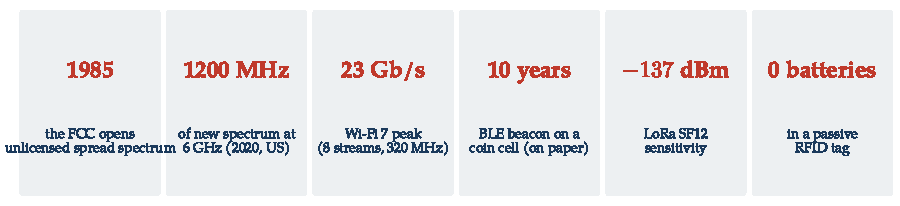
\includegraphics[width=\linewidth]{figs/ch22_by_numbers}
\caption{The chapter by the numbers. Every figure here is explained, and earned, in the pages that
follow.}\label{fig:ch22_by_numbers}
\end{figure}

\Needspace{10\baselineskip}
%======================================================================
\section{The unlicensed revolution}
\label{sec:ch22:unlicensed}
%======================================================================

Every other system in this book starts with a licence. A cellular operator pays billions for
exclusive use of a band; a broadcaster or a satellite operator holds an assignment that nobody
else may use in its coverage area. The engineer working in licensed spectrum controls the
interference environment and can plan a network around it. (Figure~\ref{fig:ch22_by_numbers} previews
a few of the numbers we will meet.)

The engineer designing a Wi-Fi chip, a Bluetooth earbud or a soil-moisture sensor cannot. The
radio must work next to an unknown number of other radios of unknown types, all with exactly the
same rights to the band. That single difference explains most of the design choices in this
chapter: listen-before-talk access, spread spectrum and frequency hopping, adaptive rates, short
packets and robust modulations. Keep it in mind; we will meet it again and again.

\mdcfig[0.98]{ch22_unlicensed_timeline}{Seventy-seven years of the unlicensed bands. For almost
four decades (compressed at the left) the ISM bands were a dumping ground for ovens and heaters.
After the FCC's 1985 decision the pace never slackened: a new Wi-Fi generation every four to six
years, Bluetooth, 802.15.4, LoRa, cellular IoT, and in 2020 the largest unlicensed allocation ever
made.}

\begin{analogy}[A public park, not a private garden]
Licensed spectrum is a private garden: one owner, a fence, and a gardener who decides what grows
where. Unlicensed spectrum is a public park. Anyone may come in, nobody may build a wall, and the
park works only because everyone follows a few rules: keep the music down, do not hog the
benches, take turns on the swings. The limit of the analogy: in a park you can see who is being
rude. A radio usually cannot, and much of this chapter is about radios guessing.
\end{analogy}

\Needspace{6\baselineskip}
\subsection{From garbage bands to a trillion-dollar industry}

The industrial, scientific and medical (\term{ISM} bands) were set aside at the 1947 International
Radio Conference in Atlantic City for non-communication uses of RF energy: diathermy machines,
industrial heaters and, later, microwave ovens. The 2.4\,GHz band was there because the domestic
microwave oven's magnetron runs at about 2450\,MHz (Figure~\ref{fig:ch22_microwave}). Communication in these bands was tolerated only
at very low power under Part~15 of the US Federal Communications Commission (FCC) rules, which
governed incidental radiators and garage-door openers. Engineers called them the ``garbage bands''.
Figure~\ref{fig:ch22_unlicensed_timeline} shows what happened next.

\mdcfig[0.8]{ch22_bands}{The three main unlicensed bands used by Wi-Fi, drawn to scale. Top: the
2.4\,GHz ISM band holds thirteen overlapping 20\,MHz Wi-Fi channels (only 1, 6 and 11 do not
overlap), forty 2\,MHz Bluetooth Low Energy channels (the three advertising channels, red, sit
at the band edges and between Wi-Fi channels 1 and 6) and sixteen 802.15.4 channels on a 5\,MHz
grid (channels 15, 20, 25 and 26, dark, fall in the gaps of the 1/6/11 plan). Middle: the
5\,GHz U-NII sub-bands and the US Wi-Fi channel plan from 20 to 160\,MHz; channels in
U-NII-2A and -2C must use dynamic frequency selection. Bottom: the 6\,GHz band offers
fifty-nine 20\,MHz channels, seven 160\,MHz channels and two interleaved sets of three
320\,MHz channels.}

\begin{history}[Michael Marcus and the 1985 decision]
In the late 1970s Michael Marcus, an engineer in the FCC's Office of Plans and Policy, argued that
spread-spectrum techniques, until then used almost exclusively by the military
(Chapter~\ref{ch:spreadspectrum}), would let many users share a band without coordination,
because each signal would look like low-level noise to the others. After a proceeding that began
in 1981 (General Docket 81-413), the Commission adopted rules in May 1985 that allowed
spread-spectrum transmitters to operate without an individual licence in the 902--928\,MHz,
2400--2483.5\,MHz and 5725--5850\,MHz ISM bands, at up to 1\,W of output power. The rules became
Section~15.247 of Part~15.

Nobody at the time predicted the result. NCR's WaveLAN (1990) and the first IEEE 802.11 radios
(1997) were spread-spectrum devices built under these rules, as were the early cordless phones and
Bluetooth. Later revisions replaced the spread-spectrum requirement with a more general ``digital
modulation'' rule, which is what allowed OFDM into the 2.4\,GHz band in 2002--03. The 1985
decision is widely regarded as one of the most economically consequential spectrum decisions ever
made, and the model of licence-exempt access under technical rules, rather than exclusive
assignment, has since been copied around the world. (The idea of hopping a radio around to dodge
jamming is much older; Chapter~\ref{ch:spreadspectrum} tells the story of Hedy Lamarr and George
Antheil's 1942 patent.)
\end{history}

\mdcphoto[0.55]{ch22_microwave}{The reason the 2.4\,GHz band exists, and still the most powerful
2.4\,GHz transmitter in most homes. The magnetron inside runs at around 2.45\,GHz behind the metal
box and the mesh in the door; the small leakage that remains, well within safety limits, is still
enormous next to a Wi-Fi packet (Section~\ref{sec:ch22:coex}).}

The model was extended in stages. The FCC created the Unlicensed National Information
Infrastructure (U-NII) bands at 5\,GHz in 1997, expanded them in 2003 and 2020, opened 57--64\,GHz
in 1995 (extended to 57--71\,GHz in 2016) and, in April 2020, made the entire 1200\,MHz from 5925 to
7125\,MHz available for unlicensed use: the largest single allocation in the history of the
unlicensed bands, and the reason Wi-Fi~6E and Wi-Fi~7 exist. Europe opened 5945--6425\,MHz
(480\,MHz) in 2021. Below 1\,GHz, the 902--928\,MHz band in the Americas and the 863--870\,MHz
short-range-device band in Europe carry LoRa, Sigfox, Z-Wave, Wi-Fi HaLow and RFID.

Figure~\ref{fig:ch22_bands} draws the three Wi-Fi bands to scale. Look first at the top panel: it
is the most crowded 83.5\,MHz on Earth, and we will come back to it many times.

\mdcfig[0.9]{ch22_psd_limit}{Two kinds of power rule. Left: under a PSD limit (6\,GHz low-power
indoor, 5\,dBm/MHz) total EIRP grows with the channel width until it hits a 30\,dBm cap; under a
fixed total (5\,GHz U-NII-3, 36\,dBm) it does not. Right: the consequence for the SNR on each
subcarrier at 80\,dB of path loss. The PSD rule makes wide channels free; the total rule makes them
cost 3\,dB per doubling.}

\Needspace{6\baselineskip}
\subsection{The rules of the commons}

Unlicensed does not mean unregulated. Each band comes with a short set of technical rules that
every device must meet, and those rules set the boundary conditions of the radio design.
Table~\ref{tab:ch22:bands} summarises the main ones; the paragraphs below explain what each rule is
for.

\paragraph{Power limits.} Rules limit the \term{equivalent isotropically radiated power} (EIRP),
the transmit power plus antenna gain, and often also the power spectral density (PSD), in dBm per
megahertz. A PSD limit means that a wider channel may carry more total power, but no more power
per hertz, so the SNR per subcarrier, and with it the range at a given MCS, stays the same as the
channel widens; under a total-power cap, by contrast, it falls by 3\,dB for each doubling of
bandwidth (Figure~\ref{fig:ch22_psd_limit}). In the 2.4\,GHz band, the FCC allows 1\,W conducted
into a 6\,dBi antenna (36\,dBm EIRP) for point-to-multipoint systems; Europe (ETSI EN~300~328)
allows only 100\,mW (20\,dBm) EIRP.

\paragraph{Dynamic frequency selection and transmit power control.} Much of the 5\,GHz band is
shared with weather, military and aviation radars. In 5250--5350 and 5470--5725\,MHz, a Wi-Fi
access point must perform \term{dynamic frequency selection} (DFS): listen for radar pulses for a
\emph{channel availability check} of 60\,s before using a channel (10\,minutes in the
5600--5650\,MHz weather-radar band in Europe), monitor continuously while operating, vacate the
channel within 10\,s of detecting a radar and stay off it for 30\,minutes
(Figure~\ref{fig:ch22_dfs}). \term{Transmit power control} (TPC) requires the ability to reduce
power below the maximum. DFS and TPC came into 802.11 with the 802.11h amendment (2003). If your
5\,GHz network ever vanished for a minute and came back on a different channel, you have probably
watched DFS at work: a false radar detection is the most common cause.

\mdcfig[0.92]{ch22_dfs}{The life cycle of a DFS channel. An access point must listen in silence
before using a radar-shared channel, keep listening while it operates, and when radar pulses
appear it must clear the channel within seconds and stay away for half an hour.}

\paragraph{6\,GHz device classes.} The 6\,GHz band is shared with fixed point-to-point microwave
links and satellite uplinks, and the FCC defined three classes of device to protect them.
\term{Low-power indoor} (LPI) access points are limited to a PSD of 5\,dBm/MHz (30\,dBm total in
320\,MHz) and must be indoor-only (no weatherproofing, no battery power, integrated antennas);
clients are limited to 6\,dB less. \term{Standard-power} devices may transmit up to 36\,dBm EIRP
(23\,dBm/MHz) in U-NII-5 and U-NII-7, indoors or out, but only on frequencies authorised by an
\term{automated frequency coordination} (AFC) system, a database that knows the location of every
licensed microwave link and computes, from the access point's geolocation, which channels and
powers are safe (Figure~\ref{fig:ch22_afc}). The first AFC systems were approved for commercial
operation in early 2024. A third class, \emph{very low power}, allows portable devices to transmit
$-5$\,dBm/MHz (14\,dBm maximum) anywhere, without AFC, for short-range uses such as phone-to-glasses
links.

\mdcfig[0.52]{ch22_afc}{Automated frequency coordination, schematically. The database knows the
path of each licensed microwave link (purple) and the protection it needs; an access point that
reports its position is granted full power on channels that cannot disturb the link, and lower
power or nothing on those that could.}

\paragraph{Listen-before-talk and duty cycle.} In Europe, ETSI harmonised standards (EN~301~893 at
5\,GHz) require \emph{adaptivity}: a device must sense the channel before transmitting and limit
its channel occupancy time. In the 868\,MHz short-range-device band (ETSI EN~300~220) there is no
listen-before-talk requirement in most sub-bands, but a transmitter may be on for at most 0.1\%,
1\% or 10\% of the time depending on the sub-band. In the US 902--928\,MHz band, frequency-hopping
systems must limit their \emph{dwell time} on any one channel to 400\,ms in a 20\,s period.
Section~\ref{sec:ch22:lora} shows how these rules shape LoRaWAN.

\begin{table}[htbp]\centering\footnotesize
\caption{The principal unlicensed bands for the systems in this chapter (United States and
Europe; maximum values, simplified; consult the regulations for detail).}
\label{tab:ch22:bands}
\begin{tabularx}{\linewidth}{@{}l l l X@{}}
\toprule
Band & Range (MHz) & Typical maximum EIRP & Main users and notes\\
\midrule
Sub-GHz (US) & 902--928 & 36\,dBm (FHSS/DTS, Part 15.247) & LoRaWAN US915, RFID, Z-Wave, HaLow; 400\,ms dwell\\
Sub-GHz (EU) & 863--870 & 14\,dBm ERP typical, 27\,dBm in 869.4--869.65 & LoRaWAN EU868, Sigfox, Z-Wave; 0.1--10\% duty cycle\\
RFID (EU) & 865--868 & 2\,W ERP & EPC Gen2 readers (ETSI EN 302 208)\\
2.4\,GHz ISM & 2400--2483.5 & 36\,dBm (US); 20\,dBm (EU) & Wi-Fi, Bluetooth, 802.15.4, microwave ovens\\
U-NII-1 & 5150--5250 & 30\,dBm (US); 23\,dBm (EU) & Wi-Fi, indoor in EU\\
U-NII-2A/2C & 5250--5350, 5470--5725 & 30\,dBm with TPC & Wi-Fi with DFS (radar)\\
U-NII-3/4 & 5725--5895 & 36\,dBm & Wi-Fi; U-NII-4 added 2020 (US)\\
6\,GHz (US) & 5925--7125 & LPI 5\,dBm/MHz; SP 36\,dBm via AFC & Wi-Fi 6E/7; also UWB at very low PSD\\
6\,GHz (EU) & 5945--6425 & 23\,dBm LPI; 14\,dBm VLP & Wi-Fi 6E/7 (ETSI EN 303 687)\\
60\,GHz & 57--71 (US) & 40\,dBm average & 802.11ad/ay, radar sensing\\
\bottomrule
\end{tabularx}
\end{table}

\begin{worked}[What a power-spectral-density limit does to a wide channel]
A 6\,GHz low-power-indoor access point is limited to 5\,dBm/MHz. What is its maximum EIRP in 20,
160 and 320\,MHz channels, and how does the received SNR per subcarrier compare?

The total EIRP is the PSD times the bandwidth: $5+10\log_{10}20=18$\,dBm in 20\,MHz,
$5+10\log_{10}160=27$\,dBm in 160\,MHz and $5+10\log_{10}320=30$\,dBm in 320\,MHz (exactly the
30\,dBm cap). Because the receiver noise also grows in proportion to bandwidth
($-174\,\text{dBm/Hz}+10\log_{10}B+\text{NF}$), the SNR is the same in all three cases: a PSD limit
makes wide channels \emph{free} in SNR terms but not \emph{better}. By contrast, at 5\,GHz in
U-NII-3 the limit is a total of 36\,dBm whatever the bandwidth (subject to a PSD cap that rarely
binds), so widening from 20 to 160\,MHz there costs 9\,dB of SNR per subcarrier. In both cases a
client is weaker than the access point: 6\,dB less in LPI, because it is limited to
$-1$\,dBm/MHz. Uplink range, not downlink, usually limits a 6\,GHz LPI network, a point taken up in
Section~\ref{sec:ch22:realworld}.
\end{worked}

\begin{keyidea}[Politeness is the price of free spectrum]
An unlicensed band is a commons, and a commons survives only if every user follows rules that
limit the harm each can do to the others. Regulators impose some rules (power, DFS, duty cycle,
dwell time); the industry imposes the rest through standards (carrier sense, random backoff,
adaptive frequency hopping). A device that ignores them, such as a jammer or a badly designed
video sender that occupies a channel continuously, can deny service to everyone within range. The
remarkable fact is how well the system works: the engineering of politeness has turned three
narrow ``garbage bands'' into the medium that carries most of the world's Internet traffic over
its final few metres.
\end{keyidea}

\Needspace{10\baselineskip}
%======================================================================
\section{Wi-Fi: architecture and evolution}
\label{sec:ch22:arch}
%======================================================================

Your home ``Wi-Fi'' is, to the standard, an extended service set with one basic service set and a
distribution system made of a single box. That sounds pompous, but the vocabulary earns its keep
the moment a house has two access points, or an office has two hundred.

\Needspace{6\baselineskip}
\subsection{Basic service sets and the distribution system}

IEEE 802.11 defines a wireless LAN as a set of \emph{stations} (STAs) that share a medium access
control (MAC) protocol and a physical layer (PHY). The building block is the \term{basic service
set} (BSS): an access point (AP) and the stations associated with it, identified by a 48-bit
\emph{BSSID} (normally the AP's MAC address). Several BSSs connected by a \term{distribution system}
(DS), usually an Ethernet switch, form an \term{extended service set} (ESS) that the user sees as
one network with one name, the \emph{SSID}. Stations can also form an \emph{independent BSS} (IBSS,
``ad hoc'' mode) without an AP, and since 802.11s (2011) a set of mesh stations can relay frames
among themselves (Figure~\ref{fig:ch22_bss}).

\begin{figure}[htbp]\centering
\begin{tikzpicture}[font=\sffamily\scriptsize,
  ap/.style={draw=navy,fill=navy!10,thick,minimum width=0.95cm,minimum height=0.55cm,rounded corners=2pt},
  sta/.style={draw=accent,fill=accent!8,circle,inner sep=1.2pt,minimum size=0.42cm},
  arr/.style={-{Stealth[length=1.6mm]},thick,navy}]
\node[draw=navy,fill=navy!4,thick,minimum width=7.6cm,minimum height=0.55cm] (ds) at (0,2.2) {Distribution system (Ethernet switch, router, Internet gateway)};
\node[ap] (ap1) at (-2.4,1.0) {AP 1};
\node[ap] (ap2) at (2.4,1.0) {AP 2};
\draw[thick,navy] (ap1) -- (ap1|-ds.south); \draw[thick,navy] (ap2) -- (ap2|-ds.south);
\draw[navy!50,dashed,thick] (-2.4,-0.05) ellipse (2.0cm and 1.25cm);
\draw[navy!50,dashed,thick] (2.4,-0.05) ellipse (2.0cm and 1.25cm);
\node[sta] (s1) at (-3.4,-0.3) {};\node[sta] (s2) at (-2.2,-0.75) {};\node[sta] (s3) at (-1.4,-0.1) {};
\node[sta] (s4) at (1.6,-0.6) {};\node[sta] (s5) at (3.3,-0.35) {};
\node[sta,fill=green!25] (s6) at (0.25,-0.45) {};
\foreach \s in {s1,s2,s3} \draw[navy!60] (ap1) -- (\s);
\foreach \s in {s4,s5} \draw[navy!60] (ap2) -- (\s);
\draw[-{Stealth[length=1.6mm]},thick,green!50!black] (s6) to[bend right=25] node[below,font=\sffamily\tiny,text=green!40!black,yshift=-1pt]{roam (802.11k/v/r)} (1.15,-0.85);
\node[text=navy] at (-2.4,-1.5) {BSS 1 (BSSID 1)};
\node[text=navy] at (2.4,-1.5) {BSS 2 (BSSID 2)};
\node[text=navy] at (0,-1.95) {Extended service set: one SSID, ``HomeNet''};
\begin{scope}[xshift=6.0cm]
\node[sta] (i1) at (0,0.9) {};\node[sta] (i2) at (0.9,0.0) {};\node[sta] (i3) at (-0.7,-0.35) {};
\draw[accent!70] (i1)--(i2)--(i3)--(i1);
\draw[accent!50,dashed,thick] (0.05,0.15) circle (1.15cm);
\node[text=accent] at (0.05,-1.4) {IBSS (ad hoc)};
\end{scope}
\end{tikzpicture}
\caption{802.11 architecture. Each access point and its associated stations form a basic service
set; a distribution system joins several BSSs into an extended service set with a single network
name, across which a station can roam. An independent BSS has no access point.}
\label{fig:ch22_bss}
\end{figure}

An AP announces itself by broadcasting a \term{beacon} frame, normally every 102.4\,ms (100
\emph{time units} of 1024\,$\mu$s), carrying the SSID, supported rates and capabilities, the channel
configuration and the traffic indication map used for power save. Ten times a second, every
access point in your street is shouting its name. A station finds networks by \emph{passive
scanning} (listening for beacons on each channel) or \emph{active scanning} (sending probe
requests), then \emph{authenticates} and \emph{associates} with the AP of its choice, and finally
completes the security handshake of Section~\ref{sec:ch22:security}. Every association, roam and
disconnection is the station's decision, not the network's, which is one of the deepest
differences from cellular systems (Chapter~\ref{ch:cellular}), where the network commands
handover.

802.11 sits below the IEEE~802.2 logical link control layer and looks to the rest of the network
like Ethernet: the same 48-bit addresses and the same EtherType payloads. The 802.11 frame has
more addresses, up to four, because a frame relayed by an AP has a transmitter and a receiver (the
radio hop) distinct from its source and destination (the Ethernet endpoints). There are three
frame types: \emph{management} (beacons, probes, authentication, association, action frames),
\emph{control} (RTS, CTS, ACK, Block Ack, trigger frames) and \emph{data}.

\Needspace{6\baselineskip}
\subsection{Twenty-five years of amendments}

The base standard, now IEEE Std 802.11-2020 with later amendments rolled in, is a document of more
than four thousand pages. It grows by \emph{amendments} named with lower-case letters (and, after
802.11z ran out the alphabet, two letters). Some define new PHYs, some MAC features, some both.
Table~\ref{tab:ch22:generations} lists the main PHY generations and the marketing names the Wi-Fi
Alliance gave them in 2018, and Figure~\ref{fig:ch22_rate_history} plots their peak rates: a factor
of ten thousand in twenty-seven years.

\begin{table}[htbp]\centering\footnotesize
\caption{The IEEE 802.11 physical-layer generations. Peak rates are the maximum defined by each
amendment (all spatial streams, widest channel, shortest guard interval); real devices with two
to four antennas reach a fraction of them.}
\label{tab:ch22:generations}
\begin{tabularx}{\linewidth}{@{}l l l l l X@{}}
\toprule
Amendment & Name & Year & Bands (GHz) & Peak rate & Key PHY features\\
\midrule
802.11 & -- & 1997 & 2.4 & 2\,Mb/s & DSSS (Barker) or FHSS; DBPSK/DQPSK\\
802.11b & (Wi-Fi 1) & 1999 & 2.4 & 11\,Mb/s & CCK at 11\,Mchip/s\\
802.11a & (Wi-Fi 2) & 1999 & 5 & 54\,Mb/s & OFDM, 64 subcarriers in 20\,MHz, up to 64-QAM\\
802.11g & (Wi-Fi 3) & 2003 & 2.4 & 54\,Mb/s & 802.11a OFDM in 2.4\,GHz, coexists with 11b\\
802.11n & Wi-Fi 4 & 2009 & 2.4, 5 & 600\,Mb/s & MIMO (4 streams), 40\,MHz, short GI, A-MPDU, LDPC\\
802.11ac & Wi-Fi 5 & 2013 & 5 & 6.9\,Gb/s & 80/160\,MHz, 256-QAM, 8 streams, DL MU-MIMO\\
802.11ax & Wi-Fi 6/6E & 2021 & 2.4, 5, 6 & 9.6\,Gb/s & OFDMA, UL MU-MIMO, 1024-QAM, 4$\times$ symbol, TWT, BSS colouring\\
802.11be & Wi-Fi 7 & 2024 & 2.4, 5, 6 & 23\,Gb/s & 320\,MHz, 4096-QAM, multi-link operation, multi-RU, puncturing\\
802.11bn & Wi-Fi 8 & $\approx$2028 & 2.4, 5, 6 & (as 11be) & Ultra-high reliability: multi-AP coordination\\
\midrule
802.11ad/ay & WiGig & 2012/21 & 60 & 6.8/$>$20\,Gb/s & 2.16\,GHz channels, beam training, SC and OFDM\\
802.11ah & HaLow & 2016 & 0.9 & 347\,Mb/s & 802.11ac downclocked by 10, 1--16\,MHz channels\\
802.11p/bd & V2X & 2010/22 & 5.9 & 27\,Mb/s (11p) & Vehicular; 10\,MHz channels\\
\bottomrule
\end{tabularx}
\end{table}

\begin{history}[From WaveLAN to Wi-Fi]
NCR's WaveLAN, developed by a team in Nieuwegein in the Netherlands and sold from 1990, was a
2\,Mb/s spread-spectrum LAN card for the 915\,MHz band (later 2.4\,GHz;
Figure~\ref{fig:ch22_wavelan}). Its engineers, led by Vic Hayes (who chaired the IEEE 802.11 working
group from its formation in 1990 until 2000) and Bruce Tuch, were central to the first 802.11
standard of 1997. That standard was too permissive to guarantee interoperability: it allowed three
different PHYs (direct sequence, frequency hopping and infrared). In 1999, as 802.11b and 802.11a
were completed, six companies (3Com, Aironet, Harris Semiconductor, Lucent, Nokia and Symbol
Technologies) formed the Wireless Ethernet Compatibility Alliance to certify interoperable
products. It hired the brand consultancy Interbrand, which proposed the name ``Wi-Fi''; the
alliance soon renamed itself after it (Figure~\ref{fig:ch22_orinoco}).

The breakthrough product came the same year: Apple's iBook, with an AirPort card based on
Lucent's 802.11b chips, for an add-on price of 99 dollars. Within five years Wi-Fi was in almost
every laptop. Australia's CSIRO, whose radio-astronomy group led by John O'Sullivan had patented
techniques for fast indoor wireless OFDM in the 1990s, later won licensing settlements worth
hundreds of millions of dollars from the industry, a reminder that the 802.11a/g/n OFDM PHY rested
on research outside the US.
\end{history}

\mdcpairany{ch22_wavelan}{An AT\&T (formerly NCR) WaveLAN card for the 915\,MHz band, a
half-length ISA board from the early 1990s. The two metal cans hold the radio; the rest is a
network card.}{ch22_orinoco}{Lucent's ORiNOCO Silver PC card, an 802.11b ``Wi-Fi'' card of about
2000. Note the logo: the Wi-Fi brand was barely a year old.}

\mdcfig[0.55]{ch22_rate_history}{Peak PHY rate of each 802.11 generation (log scale). The dotted
line is a steady tenfold gain every seven years or so. The rest of this chapter's first half
explains where each factor came from, and why the rate you actually get is so much lower.}

\Needspace{10\baselineskip}
%======================================================================
\section{The early PHYs: spread spectrum and CCK}
\label{sec:ch22:early}
%======================================================================

The original 802.11 standard gave two radio options for 2.4\,GHz, both required by the
spread-spectrum rules of the day. The \emph{frequency-hopping} PHY sent 1 or 2\,Mb/s using 2- or
4-level GFSK on 1\,MHz channels, hopping among 79 channels in the US at a rate of a few hops per
second. The \emph{direct-sequence} PHY (DSSS), which won in the market, spread each DBPSK
(1\,Mb/s) or DQPSK (2\,Mb/s) symbol by the 11-chip \term{Barker sequence}
\[
\mathbf{b}=[+1,-1,+1,+1,-1,+1,+1,+1,-1,-1,-1]
\]
at 11\,Mchip/s, occupying about 22\,MHz.

Why that particular pattern of eleven? Because it is almost perfectly unlike any shifted copy of
itself. A Barker sequence has aperiodic autocorrelation sidelobes of magnitude at most 1, against a
peak of 11 (Figure~\ref{fig:ch22_barker}), so the despreading correlator gives a clean peak for
timing and resists multipath echoes longer than one chip (91\,ns): the processing gain is
$10\log_{10}11=10.4$\,dB. The same 11\,Mchip/s, 22\,MHz-wide signal fixed the 2.4\,GHz channel plan
of Figure~\ref{fig:ch22_bands}: 5\,MHz channel spacing (inherited from earlier rules) and therefore
only three non-overlapping channels, 1, 6 and 11. A decision made for a 1997 radio still decides
where you should put your router today. Chapter~\ref{ch:spreadspectrum} develops direct-sequence
and frequency-hopping theory; here we follow how 802.11 raised the rate.

\mdcfig[0.88]{ch22_barker}{The 11-chip Barker sequence (left) and its aperiodic autocorrelation
(right). One tall peak, and every sidelobe of magnitude 0 or 1: a receiver sliding a copy of the
code past the signal knows exactly when it lines up, even with echoes around.}

\Needspace{6\baselineskip}
\subsection{Complementary code keying}

802.11b (1999) kept the 11\,Mchip/s chip rate and the spectrum mask, so that it could interoperate
with the 1 and 2\,Mb/s radios, and raised the rate to 5.5 and 11\,Mb/s with \term{complementary
code keying} (CCK). Instead of one fixed spreading code, CCK chooses each 8-chip codeword from a
family of complex codes built from four phases,
\begin{equation}
\begin{aligned}
\mathbf{c}=\big[&e^{j(\varphi_1+\varphi_2+\varphi_3+\varphi_4)},\;
e^{j(\varphi_1+\varphi_3+\varphi_4)},\;e^{j(\varphi_1+\varphi_2+\varphi_4)},\;
-e^{j(\varphi_1+\varphi_4)},\\
&e^{j(\varphi_1+\varphi_2+\varphi_3)},\;
e^{j(\varphi_1+\varphi_3)},\;-e^{j(\varphi_1+\varphi_2)},\;e^{j\varphi_1}\big].
\end{aligned}
\label{eq:ch22:cck}
\end{equation}
At 11\,Mb/s each phase takes one of four QPSK values. $\varphi_2,\varphi_3,\varphi_4$ select one of
$4^3=64$ codewords (6 bits) and $\varphi_1$, differentially encoded, rotates the whole codeword (2
more bits), so each 8-chip symbol carries 8 bits at 1.375\,Msymbol/s. At 5.5\,Mb/s only 4 bits are
carried.

The codewords are derived from Golay complementary sequences, whose autocorrelations sum to a
perfect impulse, and the 64 codewords have good mutual distance. A receiver can decide among them
with a fast Walsh-like transform (64 correlators collapsed into a butterfly structure), the same
idea as the fast Hadamard transform for orthogonal codes. CCK is better described as a block code
with 256 codewords of length 8 over the QPSK alphabet than as spreading: its ``processing gain'' at
11\,Mb/s is essentially zero, and its tolerance of multipath comes from the receiver's equaliser and
RAKE-like combining.

\begin{pitfall}[The ghost of 802.11b]
802.11b was a commercial triumph, but it left 802.11 with a legacy that still costs airtime today.
A DSSS PPDU begins with a 144\,$\mu$s preamble and a 48\,$\mu$s header sent at 1\,Mb/s (the ``long
preamble'', 192\,$\mu$s; an optional short preamble halves this), and the DSSS slot time is
20\,$\mu$s against 9\,$\mu$s for OFDM. Every 802.11g network that might contain an 802.11b station
must use the long slot and must protect its OFDM transmissions with an RTS/CTS or CTS-to-self
exchange sent at a DSSS rate that the old stations can decode. A single 802.11b client in range can
cut a 2.4\,GHz network's throughput by half or more; many enterprise networks simply disable the 1,
2, 5.5 and 11\,Mb/s rates today.
\end{pitfall}

\Needspace{6\baselineskip}
\subsection{OFDM arrives: 802.11a and g}

802.11a (1999, 5\,GHz) and 802.11g (2003, 2.4\,GHz) introduced the OFDM PHY that every later
generation extends. Its numerology is derived in Chapter~\ref{ch:ofdm}: a 64-point FFT at 20\,MS/s,
312.5\,kHz subcarrier spacing, 48 data and 4 pilot subcarriers, a 3.2\,$\mu$s useful symbol and a
0.8\,$\mu$s guard interval, for a 4\,$\mu$s symbol (Figure~\ref{fig:ch22_ofdm_subcarriers}).

\mdcfig[0.92]{ch22_ofdm_subcarriers}{The 802.11a/g subcarrier map. Of the 64 FFT bins, 48 carry data,
4 carry pilots for phase tracking, and 12 are left empty: the centre (DC) bin, which a
direct-conversion receiver cannot use, and guard bins at the edges that keep the spectrum inside its
mask. Every later generation keeps this layout in each 20\,MHz piece, only finer and wider.}

Here is the single most useful formula in Wi-Fi. In words: the rate is how many bits you put on
each subcarrier of each stream, times the number of subcarriers and streams, divided by how long
each symbol lasts. It serves every 802.11 OFDM generation:
\begin{equation}
R=\frac{N_{\text{SS}}\;N_{\text{SD}}\;N_{\text{BPSCS}}\;r}{T_{\text{sym}}},
\label{eq:ch22:rate}
\end{equation}
where $N_{\text{SS}}$ is the number of spatial streams, $N_{\text{SD}}$ the number of data
subcarriers, $N_{\text{BPSCS}}$ the coded bits per subcarrier per stream ($\log_2 M$), $r$ the code
rate and $T_{\text{sym}}$ the OFDM symbol duration including the guard interval. For 802.11a at
64-QAM with rate $3/4$: $1\times48\times6\times0.75/4\,\mu\text{s}=54$\,Mb/s. The eight 802.11a rates
(6, 9, 12, 18, 24, 36, 48 and 54\,Mb/s) are the combinations of BPSK, QPSK, 16-QAM and 64-QAM with
the $K=7$ convolutional code at rates 1/2, 2/3 and 3/4. They survive as the \emph{non-HT} rates used
for every control frame and beacon in the 5 and 6\,GHz bands.

Every later generation is a story of pushing one factor of~\eqref{eq:ch22:rate}.
Figure~\ref{fig:ch22_rate_factors} tells the whole twenty-five-year story in one picture: eight
times the streams, eighty times the subcarriers, twice the bits per subcarrier, a slightly higher
code rate, and a symbol more than three times longer, which \emph{costs} rate but buys robustness
and efficiency.

\mdcfig[0.92]{ch22_rate_factors}{From 54\,Mb/s to 23\,Gb/s by multiplying the factors of
equation~\eqref{eq:ch22:rate} one at a time. Green steps raise the rate, red lowers it. The
biggest lever by far is bandwidth (more subcarriers); the longer 802.11ax symbol gives back a factor
of 3.4 in exchange for a smaller guard-interval overhead and finer frequency resolution.}

\Needspace{10\baselineskip}
%======================================================================
\section{The PPDU: how a Wi-Fi receiver finds a packet}
\label{sec:ch22:ppdu}
%======================================================================

Imagine standing in a dark room where, at random moments, someone you have never met will shout a
sentence at you, at an unknown volume, slightly off-key, through a wall that adds echoes, in one of
five dialects. You must be ready to transcribe it from the first syllable. That is the Wi-Fi
receiver's job, and it does it tens of thousands of times a second.

A Wi-Fi receiver does not know when the next packet will arrive, how strong it will be, what
frequency error its transmitter has, what channel it has travelled through, which generation of
the standard it uses or how long it is. It must find all of this out in roughly the first
20\,$\mu$s of the packet, from a known preamble, and it must do so for every packet, because Wi-Fi
is bursty: there is no continuous downlink to stay locked to, as there is in a cellular or
broadcast system. Chapter~\ref{ch:sync} develops the estimation theory; this section shows how the
802.11 preamble packages it.

\Needspace{6\baselineskip}
\subsection{The PHY protocol data unit}

The unit of transmission is the \term{PPDU} (PHY protocol data unit): a preamble, one or more signal
fields that describe the packet, and the data field that carries the MAC's frames (the PSDU). Each
new generation has added fields after the legacy ones, so that every 802.11 OFDM packet still
begins with the same 20\,$\mu$s that an 802.11a receiver understands (Figure~\ref{fig:ch22_ppdu}).
This \emph{backward-compatible preamble} is the single most important design constraint in
Wi-Fi's evolution: it is why a 2024 Wi-Fi~7 access point can defer correctly to a 2003 laptop, and
why each new generation pays about 20\,$\mu$s of legacy overhead on every packet.

\begin{figure}[htbp]\centering
\begin{tikzpicture}[x=0.162cm,y=0.62cm,font=\sffamily\tiny,
  fld/.style={draw=white,thick,inner sep=0pt,align=center,minimum height=0.5cm}]
\def\row#1#2#3{%
  \node[anchor=east,font=\sffamily\scriptsize\bfseries,text=navy] at (-1,#1) {#2};
  \foreach \a/\b/\l/\c in {#3} {%
    \fill[\c] (\a,#1-0.4) rectangle (\b,#1+0.4);
    \draw[white,thick] (\a,#1-0.4) rectangle (\b,#1+0.4);
    \node[align=center] at ({(\a+\b)/2},#1) {\l};}}
\row{4}{Non-HT (11a/g)}{0/8/L-STF/green!30,8/16/L-LTF/orange!35,16/20/L-\\SIG/navy!25,20/34/Data/gray!20}
\row{3}{HT-mixed (11n)}{0/8/L-STF/green!30,8/16/L-LTF/orange!35,16/20/L-\\SIG/navy!25,20/28/HT-SIG/accent!25,28/32/HT-\\STF/green!15,32/40/HT-LTFs/orange!20,40/54/Data/gray!20}
\row{2}{VHT (11ac)}{0/8/L-STF/green!30,8/16/L-LTF/orange!35,16/20/L-\\SIG/navy!25,20/28/VHT-SIG-A/accent!25,28/32/VHT-\\STF/green!15,32/40/VHT-LTFs/orange!20,40/44/SIG-\\B/accent!15,44/58/Data/gray!20}
\row{1}{HE SU (11ax)}{0/8/L-STF/green!30,8/16/L-LTF/orange!35,16/20/L-\\SIG/navy!25,20/24/RL-\\SIG/navy!15,24/32/HE-SIG-A/accent!25,32/36/HE-\\STF/green!15,36/52/HE-LTFs/orange!20,52/66/Data/gray!20,66/70/PE/gray!8}
\row{0}{EHT MU (11be)}{0/8/L-STF/green!30,8/16/L-LTF/orange!35,16/20/L-\\SIG/navy!25,20/24/RL-\\SIG/navy!15,24/32/U-SIG/accent!25,32/40/EHT-SIG/accent!15,40/44/EHT-\\STF/green!15,44/60/EHT-LTFs/orange!20,60/74/Data/gray!20,74/78/PE/gray!8}
\draw[decorate,decoration={brace,amplitude=4pt},navy] (0,4.55) -- (20,4.55) node[midway,above=4pt,font=\sffamily\scriptsize,text=navy]{legacy preamble, 20\,$\mu$s};
\draw[navy!60,dashed] (20,-0.6) -- (20,4.5);
\foreach \t in {0,10,20,30,40,50,60,70}{\draw[gray] (\t,-0.55) -- (\t,-0.65) node[below,font=\sffamily\tiny,text=gray]{\t};}
\node[font=\sffamily\tiny,text=gray] at (80,-0.85) {$\mu$s};
\end{tikzpicture}
\caption{PPDU formats of five 802.11 OFDM generations, roughly to scale (two spatial streams; the
data field is truncated). Every format begins with the legacy short and long training fields and
the legacy signal field, which older receivers use to detect the packet and to compute how long
to stay off the air. Later fields add signalling for the new format (HT-SIG, VHT-SIG-A, HE-SIG-A,
U-SIG and EHT-SIG), a new short training field for re-adjusting the gain over the wider or
beamformed channel, and one long training field per spatial stream for MIMO channel estimation.
HE and EHT packets end with an optional packet extension (PE) that gives receivers extra time
to finish decoding.}
\label{fig:ch22_ppdu}
\end{figure}

\Needspace{6\baselineskip}
\subsection{The legacy short training field}

The \term{L-STF} is an OFDM symbol that uses only 12 of the 52 subcarriers, every fourth one
($\pm4,\pm8,\dots,\pm24$), with QPSK values chosen for a low peak-to-average ratio. Occupying every
fourth subcarrier makes the time signal periodic with period $64/4=16$ samples, or 0.8\,$\mu$s, and
the field contains ten repetitions, 8\,$\mu$s in all: a short tune hummed ten times, so that a
listener who misses the start can still recognise it. The receiver uses it for four jobs in
sequence:

\mdcfig{ch22_preamble_sync}{Packet detection on a simulated 802.11 legacy preamble with a
three-path channel, an 80\,kHz carrier frequency offset and 10\,dB SNR (generated with the
standard's L-STF and L-LTF sequences). Top: the received envelope. Middle: the normalised
delay-16 autocorrelation~\eqref{eq:ch22:sc} rises to a plateau during the short training
field, independent of the channel and the signal level. Bottom: after coarse frequency
correction, cross-correlation with the known 3.2\,$\mu$s long training symbol gives two sharp
peaks that fix the symbol timing; the smaller peaks are the echoes of the multipath channel and
the cyclic prefix.}

\begin{enumerate}
\item \textbf{Packet detection.} A periodic signal correlates with itself delayed by one period;
noise does not. The \emph{delay-and-correlate} detector computes
\begin{equation}
P(n)=\sum_{k=0}^{L-1}r[n+k]\,r^*[n+k+D],\qquad
R(n)=\sum_{k=0}^{L-1}|r[n+k+D]|^2,\qquad
M(n)=\frac{|P(n)|^2}{R(n)^2},
\label{eq:ch22:sc}
\end{equation}
with $D=16$ samples, and declares a packet when $M(n)$ exceeds a threshold
(Figure~\ref{fig:ch22_preamble_sync}). Because $M(n)$ is normalised by the received energy, the
threshold does not depend on the signal level, which is unknown at this stage. Because it compares
the signal with itself, it is unaffected by the multipath channel: a periodic signal passed through
any channel shorter than the period is still periodic. This is the Schmidl--Cox idea of
Chapter~\ref{ch:sync}.
\item \textbf{Automatic gain control.} Received power can be anywhere from $-90$ to $-20$\,dBm, and
the ADC has perhaps 50--60\,dB of useful dynamic range. The AGC measures the power during the first
few STF periods and sets the analogue gain, typically in two or three steps, before the long
training field arrives. Two to three microseconds of the STF are usually spent this way.
\item \textbf{Coarse frequency offset.} The 802.11 standard allows each oscillator an error of
$\pm20$\,ppm, so at 5.8\,GHz the transmitter and receiver can differ by up to
$40\times10^{-6}\times5.8\times10^9=232$\,kHz, almost a whole subcarrier spacing (312.5\,kHz). A
frequency offset $\Delta f$ rotates each sample by $2\pi\Delta f T_s$, so after $D$ samples the
correlation $P(n)$ has the phase $-2\pi\Delta f DT_s$ and
\begin{equation}
\widehat{\Delta f}=-\frac{\angle P(n)}{2\pi DT_s}.
\label{eq:ch22:cfo}
\end{equation}
The phase is unambiguous for $|\Delta f|<1/(2DT_s)=625$\,kHz, comfortably larger than the worst
case.
\item \textbf{Coarse timing.} The end of the plateau in $M(n)$ marks the end of the STF to within a
few samples.
\end{enumerate}

\begin{tryit}[Find the packet yourself]
Open Lab~31 (\texttt{lab31\_wifi\_ble\_lora.py}) and choose ``802.11 preamble: find, tune, measure''.
Lower the SNR slider towards 0\,dB and watch the autocorrelation plateau sink into the noise; raise
the detection-threshold slider until packets start being missed. Then drag the carrier-frequency-offset
slider past $\pm156$\,kHz and switch the multipath menu between channels: the coarse STF estimate
survives, the fine LTF-only estimate wraps. Tick ``Average the two LTF symbols'' and see the
channel estimate tidy up.
\end{tryit}

\Needspace{6\baselineskip}
\subsection{The legacy long training field and signal field}

\mdcfig[0.5]{ch22_ltf_estimate}{A least-squares channel estimate from the L-LTF on a simulated
three-path channel at 10\,dB SNR. One symbol gives a noisy estimate (orange); averaging the two
identical LTF symbols halves the noise power (navy) and follows the true channel (grey) closely,
deep fade included.}

The \term{L-LTF} is a 1.6\,$\mu$s guard interval followed by two identical 3.2\,$\mu$s OFDM symbols
carrying known BPSK values on all 52 subcarriers. It serves three purposes:
\begin{itemize}
\item \textbf{Fine timing}, by cross-correlating with the known symbol (bottom panel of
Figure~\ref{fig:ch22_preamble_sync}).
\item \textbf{Fine frequency offset}, by applying~\eqref{eq:ch22:cfo} with $D=64$: four times the
averaging length and therefore much better accuracy, but an unambiguous range of only
$\pm156$\,kHz, which is why the coarse STF estimate must come first.
\item \textbf{Channel estimation}, by dividing the FFT of the (averaged) two symbols by the known
values, which gives a least-squares estimate of the channel on every subcarrier with 3\,dB of
averaging gain (Chapter~\ref{ch:ofdm}; Figure~\ref{fig:ch22_ltf_estimate}). This estimate is used to equalise the rest of the packet,
with the four pilot subcarriers tracking residual phase drift.
\end{itemize}

The \term{L-SIG} field is one BPSK, rate-1/2 OFDM symbol carrying 24 bits: a 4-bit RATE, a 12-bit
LENGTH in bytes, a parity bit and six tail bits. Together, RATE and LENGTH tell any receiver how
long the packet will occupy the medium. Later formats exploit this: an 802.11n, ac, ax or be
transmitter sets L-SIG to the 6\,Mb/s rate and a fictitious length chosen so that a legacy receiver
computes the correct duration and stays quiet, even though it cannot decode anything after L-SIG.
This \emph{spoofing} is what makes the mixed-format preamble work, and it limits a PPDU to the
longest duration that L-SIG can express, about 5.484\,ms.

\mdcfig[0.85]{ch22_format_detect}{Telling the formats apart by rotation (simulated symbols after
L-SIG, 48 subcarriers each). A legacy signal field is BPSK on the real axis; 802.11n's HT-SIG is
the same BPSK turned 90° (QBPSK); 802.11ac's VHT-SIG-A uses BPSK in its first symbol and QBPSK in
its second. Measuring where the energy lies takes the receiver one or two symbols.}

\begin{analogy}[``I will be speaking for 3 milliseconds'']
L-SIG is like a speaker at a multilingual meeting who begins every speech, in the one language
everybody shares, with ``what follows is in Finnish and will take three minutes''. Delegates who do
not speak Finnish cannot follow, but they know exactly how long to wait before raising their hand.
The limit: real delegates may get bored and interrupt; a legacy Wi-Fi station never does.
\end{analogy}

\Needspace{6\baselineskip}
\subsection{Telling the formats apart}

After L-SIG, a receiver must decide within a symbol or two which format it is receiving. The
designers used constellation rotation as a signalling trick (Figure~\ref{fig:ch22_format_detect}). HT-SIG is sent with \emph{QBPSK},
BPSK rotated by 90° onto the imaginary axis, so that energy in the quadrature component of the first
symbol after L-SIG identifies an 802.11n packet. VHT-SIG-A uses BPSK in its first symbol and QBPSK in
its second. 802.11ax sends a repeated copy of L-SIG (RL-SIG) right after L-SIG; a receiver that sees
the repetition knows the packet is HE or later. 802.11be introduced the \emph{universal signal
field} (U-SIG), whose first part carries version-independent bits (PHY version, bandwidth, BSS
colour, TXOP duration) intended to remain in the same place in all future generations, so that a
Wi-Fi~8 receiver can understand the essentials of a Wi-Fi~9 packet.

The fields after the format-specific signalling are a new short training field (HT-STF, VHT-STF,
HE-STF, EHT-STF), used to re-run the AGC over the full bandwidth and with the beamformed or MIMO
signal, and one long training field per spatial stream (HT-LTF and its successors). The LTFs are
multiplied across streams by an orthogonal $\mathbf{P}$ matrix, so that the receiver can separate
the channel from each transmit stream to each receive antenna, the $N_r\times N_{\text{SS}}$ matrix
needed for MIMO detection (Chapter~\ref{ch:mimo}).

\begin{worked}[The preamble budget of a short packet]
A smartphone sends a 100-byte TCP acknowledgement to an 802.11ax access point at 2 spatial streams,
MCS~7 (64-QAM, rate 5/6) in 80\,MHz. How long is the PPDU, and what fraction is preamble?

From~\eqref{eq:ch22:rate}, with 980 data subcarriers and a 13.6\,$\mu$s symbol, each symbol carries
$2\times980\times6\times5/6=9800$ bits. The PSDU, a 100-byte payload plus about 40 bytes of MAC
header, security and delimiter, is roughly 1120 bits plus 22 bits of service and tail: a single
data symbol. The HE SU preamble is $8+8+4+4+8+4+2\times8=52$\,$\mu$s (L-STF, L-LTF, L-SIG, RL-SIG,
HE-SIG-A, HE-STF and two 8\,$\mu$s HE-LTFs with 2$\times$ compression and 1.6\,$\mu$s guard). The
packet lasts about $52+13.6=66$\,$\mu$s, of which 79\% is preamble, and the airtime would be almost
the same at MCS~0.

For small packets, the PHY rate is nearly irrelevant: what matters is how many packets can share
one preamble (Figure~\ref{fig:ch22_preamble_overhead}). That is the motivation for aggregation
(Section~\ref{sec:ch22:mac}) and for 802.11ax OFDMA, which lets many stations share one preamble in
the frequency domain.
\end{worked}

\mdcfig[0.55]{ch22_preamble_overhead}{The preamble tax: the fraction of a PPDU's airtime spent on
its 52\,$\mu$s HE preamble, versus the size of the PSDU, for three MCSs. A TCP acknowledgement is
almost all preamble at any rate; only aggregates of many kilobytes make the preamble negligible.}

\Needspace{10\baselineskip}
%======================================================================
\section{High throughput: 802.11n and 802.11ac}
\label{sec:ch22:htvht}
%======================================================================

\Needspace{6\baselineskip}
\subsection{802.11n: MIMO comes to the mass market}

802.11n (Wi-Fi~4, 2009, though ``draft-n'' products shipped from 2007) multiplied the peak rate by
more than ten with a set of independent improvements, each of which shows up as a factor
in~\eqref{eq:ch22:rate}:
\begin{itemize}
\item \textbf{More subcarriers:} 52 data subcarriers (instead of 48) in 20\,MHz, by using more of the
band, and an optional 40\,MHz channel with 108 data subcarriers, made by bonding two adjacent
20\,MHz channels and filling in the gap between them.
\item \textbf{Higher code rate:} a rate-5/6 puncturing of the convolutional code, so the top
modulation and coding scheme (MCS) became 64-QAM rate 5/6.
\item \textbf{Short guard interval:} an optional 0.4\,$\mu$s guard interval, cutting the symbol from
4.0 to 3.6\,$\mu$s, for indoor channels whose delay spread allows it.
\item \textbf{Spatial multiplexing:} up to four spatial streams with four antennas at each end
(Chapter~\ref{ch:mimo}), with the HT-LTF fields providing the MIMO channel estimate.
\end{itemize}
The peak rate follows directly: $4\times108\times6\times\tfrac56/3.6\,\mu\text{s}=600$\,Mb/s.
802.11n also added an optional LDPC code (about 1.5--2\,dB better than the convolutional code at
the same rate; Chapter~\ref{ch:moderncodes}), space--time block coding (Alamouti, for diversity when
the receiver has fewer antennas than the transmitter), transmit beamforming (explicit, with channel
feedback, and implicit, using reciprocity; neither was widely implemented in 802.11n products) and,
crucially, frame aggregation and block acknowledgement, without which, as
Section~\ref{sec:ch22:mac} shows, the higher PHY rates would have been almost useless.

\Needspace{6\baselineskip}
\mdcfig[0.55]{ch22_mumimo_beams}{Zero-forcing precoding from an eight-antenna access point to three
single-antenna stations (dotted directions, free-space line-of-sight model). Each coloured beam
points energy at its own station and places nulls on the other two. Radius is gain in decibels over a
30\,dB range.}

\subsection{802.11ac: wider, denser, multi-user}

802.11ac (Wi-Fi~5, 2013) is a 5\,GHz-only amendment that pushed every factor further: 80\,MHz
channels (234 data subcarriers) and 160\,MHz or non-contiguous 80+80\,MHz (468), 256-QAM at rates
3/4 and 5/6, and up to eight spatial streams. The headline rate is
$8\times468\times8\times\tfrac56/3.6\,\mu\text{s}\approx6.93$\,Gb/s. Practical first-wave products had
three streams at 80\,MHz (1.3\,Gb/s); smartphones had one or two (433 or 867\,Mb/s).

The more profound change was \term{downlink multi-user MIMO} (DL MU-MIMO), introduced with the
``Wave~2'' products from about 2016. An access point with $N_t$ antennas can send different streams
to up to four stations at once, each with one or two antennas, by precoding so that each station
receives its own streams with little interference from the others
(Figure~\ref{fig:ch22_mumimo_beams}). Think of a waiter who can pour three different drinks into
three glasses at once by aiming three bottles, each carefully tilted away from the other two glasses.
The principle is the zero-forcing or regularised precoding of Chapter~\ref{ch:mimo}; the
Wi-Fi-specific part is how the AP learns the channel.

\Needspace{6\baselineskip}
\subsection{Channel sounding}

Precoding requires the transmitter to know the downlink channel. 802.11ac standardised a single
explicit procedure, \term{sounding} (Figure~\ref{fig:ch22_sounding}):
\begin{enumerate}
\item The AP sends a \emph{null data packet announcement} (NDPA) naming the stations to be sounded.
\item A short interframe space later it sends a \emph{null data packet} (NDP): a VHT preamble with
one LTF per transmit antenna and no data field.
\item Each station estimates the $N_r\times N_t$ channel matrix $\mathbf{H}_k$ on each subcarrier
group, computes its singular value decomposition
$\mathbf{H}_k=\mathbf{U}_k\boldsymbol{\Sigma}_k\mathbf{V}_k^H$, and returns the right singular vectors
$\mathbf{V}_k$ compressed into a set of Givens rotation angles (typically 4--9 bits each), together
with the per-stream SNR, in a \emph{compressed beamforming report}. For MU-MIMO the AP polls the
stations one by one with \emph{beamforming report poll} frames.
\item The AP computes a precoder (for example zero forcing over the reported $\mathbf{V}_k$) and
transmits.
\end{enumerate}

\begin{figure}[htbp]\centering
\begin{tikzpicture}[x=0.78cm,y=0.7cm,font=\sffamily\scriptsize]
\node[anchor=east,text=navy,font=\sffamily\scriptsize\bfseries] at (-0.2,2) {AP};
\node[anchor=east,text=navy,font=\sffamily\scriptsize\bfseries] at (-0.2,1) {Station 1};
\node[anchor=east,text=navy,font=\sffamily\scriptsize\bfseries] at (-0.2,0) {Station 2};
\foreach \y in {0,1,2} \draw[gray!50] (0,\y-0.3) -- (15.6,\y-0.3);
\fill[accent!40] (0,1.7) rectangle (1.6,2.3); \node at (0.8,2) {NDPA};
\fill[orange!45] (2.0,1.7) rectangle (4.2,2.3); \node at (3.1,2) {NDP (LTFs)};
\fill[green!40] (4.6,0.7) rectangle (7.2,1.3); \node at (5.9,1) {BF report 1};
\fill[accent!25] (7.6,1.7) rectangle (8.9,2.3); \node at (8.25,2) {poll};
\fill[green!40] (9.3,-0.3) rectangle (11.9,0.3); \node at (10.6,0) {BF report 2};
\fill[navy!45] (12.3,1.7) rectangle (15.6,2.3); \node[text=white] at (13.95,2) {MU-MIMO data};
\draw[decorate,decoration={brace,amplitude=4pt,mirror},gray] (0,-0.55) -- (11.9,-0.55) node[midway,below=4pt,text=gray]{sounding overhead, repeated every few tens of milliseconds};
\end{tikzpicture}
\caption{An 802.11ac/ax sounding exchange. The AP announces and sends a null data packet; each
station measures the channel and returns a compressed beamforming report, the second only when
polled. Only then can the precoded multi-user transmission begin. Everything before the navy block
is overhead.}
\label{fig:ch22_sounding}
\end{figure}
The angle representation exploits the fact that $\mathbf{V}$ is unitary: an $N_t\times N_c$ unitary
matrix is described by $N_c(2N_t-N_c-1)$ real angles rather than $2N_tN_c$ real numbers. Even so,
sounding is expensive: with 8 AP antennas, 2 streams per station and 4 stations, the reports can
amount to tens of kilobits per sounding, and if the channel changes (a person walks by) faster than
the sounding interval, the precoder goes stale and the inter-user interference rises. This feedback
overhead and staleness is the main reason MU-MIMO gains in real Wi-Fi networks have been well below
the theoretical ones.

\mdcfig[0.95]{ch22_ru_tiling}{Top: the 802.11ax resource-unit layouts within one 20\,MHz channel.
Nine 26-tone RUs (about 2\,MHz each, with the centre RU straddling the DC null), four 52-tone RUs,
two 106-tone RUs (each with the centre 26-tone RU) or one 242-tone RU; the AP may mix sizes, and
wider channels repeat the pattern and add 484-, 996- and 2$\times$996-tone RUs. Bottom: 802.11be
preamble puncturing, in which part of a wide channel is left empty because an incumbent (here a
radar or a neighbouring network) is using it, instead of falling back to a narrower channel.}

\begin{inpractice}[Why your laptop has two antennas]
Most phones and laptops have two Wi-Fi antennas and support two spatial streams; access points have
four to twelve. A 2$\times$2 client gets the second stream only when the channel is rich enough in
scattering and strong enough to support two streams at a good MCS, typically within one or two
rooms of the AP. Beyond that, the second antenna still earns its keep by receive diversity and by
maximal-ratio combining, which adds about 3\,dB of array gain and, more importantly, removes deep
fades (Chapter~\ref{ch:channels}). Extra AP antennas serve MU-MIMO, transmit beamforming (which
improves SNR at the client by focusing energy, typically by 3--6\,dB with four or more antennas), and
uplink reception diversity.
\end{inpractice}

\Needspace{10\baselineskip}
%======================================================================
\section{Wi-Fi 6, 6E, 7 and beyond}
\label{sec:ch22:he}
%======================================================================

By the mid-2010s, Wi-Fi's problem was no longer peak rate but efficiency in crowded deployments:
apartment blocks with dozens of overlapping networks, stadiums, offices with a hundred clients per
AP, and traffic dominated by small packets. Ask anyone why their Wi-Fi is slow in a hotel and the
honest answer is rarely ``the radio is too slow''. It is ``too many people are talking''. The
802.11ax task group was named ``High Efficiency WLAN'', and its metric was average throughput per
station in dense scenarios, not peak rate.

\Needspace{6\baselineskip}
\subsection{802.11ax: OFDMA, uplink MU and the 4$\times$ symbol}

Chapter~\ref{ch:ofdm} described the change in numerology: subcarrier spacing cut by four to
78.125\,kHz, a 12.8\,$\mu$s symbol and guard intervals of 0.8, 1.6 or 3.2\,$\mu$s. The longer symbol
cuts the guard overhead (from 11\% with the 0.4\,$\mu$s short GI of 11n/ac to 5.9\% with 0.8\,$\mu$s),
makes outdoor operation with 3.2\,$\mu$s practical and uses more of the channel (242 subcarriers out
of 256 in 20\,MHz against 56 out of 64). The MAC-level changes matter more.

\paragraph{OFDMA and resource units.} The AP can divide a channel into \term{resource units} (RUs)
of 26, 52, 106, 242, 484, 996 or $2\times996$ tones (Figure~\ref{fig:ch22_ru_tiling}) and serve a
different station in each, all within one PPDU with one preamble. The smallest RU is about 2\,MHz
wide, so a 20\,MHz channel can carry nine stations at once and a 160\,MHz channel seventy-four. For
the many short packets of real traffic (acknowledgements, voice frames, sensor reports, game
updates), this converts one preamble per packet into one preamble per group of packets
(Figure~\ref{fig:ch22_ofdma}): instead of nine delivery vans each carrying one letter, one van with
nine compartments.

\mdcfig[0.95]{ch22_ofdma}{Nine short packets to nine stations, drawn to scale (approximate
802.11ax timings). Top: one at a time, each paying contention, a preamble (orange) and an
acknowledgement. Bottom: all nine in one OFDMA PPDU, each in its own 26-tone resource unit, with a
single preamble and one multi-station acknowledgement. The airtime falls by a factor of about five.}

\paragraph{Uplink multi-user transmission.} OFDMA and MU-MIMO in the uplink require that several
stations transmit in the same PPDU, aligned in time to within the guard interval, in frequency to a
small fraction of the subcarrier spacing and in power to within a few decibels. 802.11ax achieves
this with the \term{trigger frame}: the AP sends a frame that allocates RUs (or MU-MIMO spatial
streams), MCSs, lengths and target received powers to a list of stations, and each named station
transmits its \emph{trigger-based PPDU} exactly one SIFS after the end of the trigger, having
corrected its frequency to the AP's and set its power from the measured path loss. This is a
fragment of cellular scheduling transplanted into Wi-Fi, and it requires the AP to know who has
data to send: \emph{buffer status report polls} and \emph{random-access RUs} let stations report
their queues. In practice, uplink OFDMA has been deployed much more cautiously than downlink,
because a station's timing and power errors hurt every other station in the same PPDU.

\paragraph{BSS colouring and spatial reuse.} In a dense deployment, a station often hears packets
from a neighbouring network (an \emph{overlapping BSS}, OBSS) just above the $-82$\,dBm
preamble-detection threshold and defers to them, even though transmitting would not disturb them.
802.11ax adds a 6-bit \term{BSS colour} to HE-SIG-A, so that a receiver can tell within the first few
microseconds whether a packet comes from its own BSS. If it is from another colour and weaker than an
\emph{OBSS power-detection} threshold, which may be raised from $-82$ up to $-62$\,dBm, the station
can ignore it and resume its backoff, provided it reduces its own transmit power in proportion to
how far it raised the threshold. The rule trades a little range for more simultaneous
transmissions; its benefit depends strongly on the topology. It is the radio version of two quiet
conversations at opposite ends of a long table: each group may ignore the other's murmur, provided
nobody raises their voice (Figure~\ref{fig:ch22_obss_pd}).

\mdcfig[0.5]{ch22_obss_pd}{The spatial-reuse bargain of 802.11ax, as specified with a reference power
of 21\,dBm: for every decibel a station raises its OBSS preamble-detection threshold above
$-82$\,dBm, it must lower its transmit power by one decibel.}

\paragraph{Target wake time.} Borrowed from 802.11ah, \term{target wake time} (TWT) lets a station
negotiate with the AP specific times at which it will wake to exchange frames, for example every
30\,s for a sensor or every 10\,ms for a game controller. Between those times the station's radio
can be completely off. TWT also lets the AP spread clients' wake times so that they do not contend
at once, a form of scheduling (Figure~\ref{fig:ch22_twt}).

\mdcfig[0.92]{ch22_twt}{Target wake time: each station agrees a private timetable with the access
point. A sensor wakes twice a minute, a thermostat every few seconds, a game controller a hundred
times a second; between their service periods their radios are off, and the AP can stagger the
schedules so the stations never contend with each other.}

\paragraph{Other features.} 1024-QAM (MCS~10 and 11; Table~\ref{tab:ch09:wifimcs}), \emph{dual
carrier modulation} (DCM, which repeats each bit on two widely separated subcarriers for frequency
diversity at the lowest rates), an \emph{extended-range} SU format with a boosted preamble for
outdoor links, mid-packet \emph{midambles} for tracking channel changes at vehicular speed, and
uplink MU-MIMO. Wi-Fi~6E is simply 802.11ax in the 6\,GHz band; the Wi-Fi Alliance requires that
6\,GHz devices support WPA3 and that legacy (pre-ax) devices are not admitted, so the 6\,GHz band
carries no 802.11b-style baggage.

\Needspace{6\baselineskip}
\subsection{802.11be: Wi-Fi 7}

802.11be, ``Extremely High Throughput'' (EHT, 2024; Wi-Fi Alliance certification began in January
2024), keeps the 802.11ax numerology and adds:
\begin{itemize}
\item \textbf{320\,MHz channels} in 6\,GHz (3920 data subcarriers per stream), doubling
$N_{\text{SD}}$.
\item \textbf{4096-QAM} (MCS~12 and 13), which needs about 38\,dB of SNR including transmitter EVM;
Lab~11 computes the EVM budget.
\item \textbf{Multi-RU and preamble puncturing.} A station may be assigned several RUs, and a wide
transmission may skip a 20\,MHz (or larger) subchannel occupied by an incumbent
(Figure~\ref{fig:ch22_ru_tiling}). Puncturing was introduced for DL MU in 802.11ax but is general in
11be; it is especially valuable in 5\,GHz, where a single DFS radar detection in a 160\,MHz channel
would otherwise force a fall-back to 80\,MHz.
\item \textbf{Multi-link operation} (MLO), the headline MAC feature, described below.
\item \textbf{More spatial streams in signalling.} The early 802.11be proposals targeted sixteen
spatial streams, which gives the widely quoted 46\,Gb/s; the amendment as completed supports up to
eight, for a peak of $8\times3920\times12\times\tfrac56/13.6\,\mu\text{s}\approx23$\,Gb/s.
\end{itemize}

\mdcfig[0.92]{ch22_mlo_links}{Multi-link operation in one picture. A frame arrives while all three
links are busy with other traffic (grey); a multi-link device sends it on whichever link falls
silent first, here 2.4\,GHz, instead of waiting for the one band it happened to be associated on.}

\begin{tryit}[How clean must a 4096-QAM transmitter be?]
Open Lab~11 (\texttt{lab11\_air\_interfaces.py}) and choose ``4096-QAM: the EVM budget''. Set the
modulation menu to 4096-QAM with ``Zoom on one corner'' ticked, then drag the transmitter-EVM slider
from $-36$ towards $-30$\,dB and watch the corner points smear into each other. Raise the receiver
SNR slider to 55\,dB: it no longer helps, because the transmitter's own noise sets the floor. Add a
little phase noise and see the outer points rotate first.
\end{tryit}

\paragraph{Multi-link operation.} Before 802.11be, a station was associated on one band at a time.
A \term{multi-link device} (MLD) has one MAC identity but several affiliated radios, one per
\emph{link} (for example 2.4, 5 and 6\,GHz), and associates once over all of them. Frames from one
traffic queue can then be sent on whichever link becomes free first, or on several at once, like a
shopper who joins whichever of three checkout queues moves first (Figure~\ref{fig:ch22_mlo_links}).
The modes differ in hardware cost:
\begin{itemize}
\item \emph{Simultaneous transmit and receive} (STR): independent radios on well-separated bands,
each running its own channel access; throughput adds, and latency falls because a frame waits only
for the first free link.
\item \emph{Non-STR} (NSTR): for links too close in frequency (for example two 5\,GHz channels) for
one device to transmit on one while receiving on the other, transmissions are aligned so that the
PPDUs on both links start and end together.
\item \emph{Enhanced multi-link single radio} (EMLSR): a device with one full radio listens on two or
more links with reduced capability (for example one antenna each) and, as soon as an initial control
frame arrives on one link, switches all its antennas to that link for the exchange. This gives most
of MLO's latency benefit at the cost of one radio, and it is the mode most phones implemented first.
\end{itemize}
The main benefit of MLO is not peak throughput but \emph{latency and reliability}: when a microwave
oven, a neighbour's video stream or a DFS event blocks one link, traffic continues on another
without reassociation. Figure~\ref{fig:ch22_mlo} puts a number on it with a toy model.

\mdcpairany{ch22_mlo}{Channel-access delay with one link and with three (a toy model: each link is
busy with neighbours' traffic about half the time, and the 5\,GHz link is occasionally blocked for
tens of milliseconds). The median barely changes; the tail collapses.}{ch22_mesh_nodes}{A
two-node consumer mesh system (router and point). Systems like this, and the tri-band Wi-Fi~7
routers that followed, use extra radios or MLO for the wireless link between the nodes
(Section~\ref{sec:ch22:mac}).}

\begin{worked}[Wi-Fi 7 for a real phone]
Chapter~\ref{ch:ofdm} computed the headline rates of Wi-Fi~6 and~7. What does a two-stream Wi-Fi~7
phone see, using MLO across a 320\,MHz channel at 6\,GHz and a 160\,MHz channel at 5\,GHz?

With 2 streams at MCS~13 and the 0.8\,$\mu$s guard, equation~\eqref{eq:ch22:rate} gives
$2\times3920\times12\times\tfrac56/13.6\,\mu\text{s}=5.76$\,Gb/s on the 320\,MHz link and
$2\times1960\times12\times\tfrac56/13.6\,\mu\text{s}=2.88$\,Gb/s on the 160\,MHz link: 8.6\,Gb/s of PHY
rate in total. Three things reduce it. First, MCS~13 needs about 38\,dB of SNR, which in the LPI
6\,GHz band with a 320\,MHz noise bandwidth (noise floor about $-174+85+7=-82$\,dBm) means a received
signal of $-44$\,dBm: line of sight within a few metres. Second, MAC overhead:
Section~\ref{sec:ch22:mac} shows that even with 256-MPDU aggregates, a 5.8\,Gb/s link achieves about
70\% MAC efficiency. Third, the phone's TCP/IP stack and application must keep up. Measured
single-device throughputs of 3--5\,Gb/s in ideal conditions are consistent with this arithmetic; one
room away, at MCS~7--9 on each link, the total falls to 2--3\,Gb/s.
\end{worked}

\Needspace{6\baselineskip}
\subsection{802.11bn: Wi-Fi 8 and ultra-high reliability}

\begin{figure}[htbp]\centering
\begin{tikzpicture}[font=\sffamily\scriptsize,>={Stealth[length=1.6mm]}]
\begin{scope}
\node[font=\sffamily\scriptsize\bfseries,text=navy] at (1.5,2.0) {Today: contend blindly};
\node[draw=navy,fill=navy!15,thick,minimum width=0.8cm,minimum height=0.45cm] (a1) at (0,1) {AP 1};
\node[draw=navy,fill=navy!15,thick,minimum width=0.8cm,minimum height=0.45cm] (a2) at (3,1) {AP 2};
\node[circle,draw=accent,fill=accent!15,inner sep=1.5pt] (c1) at (1.1,0) {};
\node[circle,draw=green!50!black,fill=green!15,inner sep=1.5pt] (c2) at (1.9,0) {};
\draw[->,thick,navy] (a1) -- (c1); \draw[->,thick,navy] (a2) -- (c2);
\draw[->,thick,accent,dashed] (a1) -- (c2); \draw[->,thick,accent,dashed] (a2) -- (c1);
\node[text=accent] at (1.5,-0.5) {each AP's signal hits the other's client};
\end{scope}
\begin{scope}[xshift=6.2cm]
\node[font=\sffamily\scriptsize\bfseries,text=navy] at (1.5,2.0) {Wi-Fi 8: coordinate};
\node[draw=navy,fill=navy!15,thick,minimum width=0.8cm,minimum height=0.45cm] (b1) at (0,1) {AP 1};
\node[draw=navy,fill=navy!15,thick,minimum width=0.8cm,minimum height=0.45cm] (b2) at (3,1) {AP 2};
\node[circle,draw=accent,fill=accent!15,inner sep=1.5pt] (d1) at (1.1,0) {};
\node[circle,draw=green!50!black,fill=green!15,inner sep=1.5pt] (d2) at (1.9,0) {};
\draw[->,thick,navy] (b1) -- (d1); \draw[->,thick,navy] (b2) -- (d2);
\draw[dotted,gray] (b1) -- (d2) node[pos=0.75,sloped,above,font=\sffamily\tiny]{null};
\draw[dotted,gray] (b2) -- (d1) node[pos=0.75,sloped,above,font=\sffamily\tiny]{null};
\draw[<->,orange,thick] (b1) to[bend left=30] node[above,font=\sffamily\tiny]{share schedule, power, nulls} (b2);
\node[text=green!40!black] at (1.5,-0.5) {both transmit at once, cleanly};
\end{scope}
\end{tikzpicture}
\caption{The idea behind Wi-Fi~8's multi-AP coordination, sketched. Neighbouring access points that
talk to each other can steer nulls towards each other's clients, agree on power levels or take
turns, instead of treating each other as anonymous interference.}
\label{fig:ch22_multiap}
\end{figure}

The 802.11bn task group, ``Ultra High Reliability'' (UHR), began work in 2023 with a target
completion around 2028. Its goal is not a higher peak rate (it keeps 320\,MHz, 4096-QAM and eight
streams) but better tail performance: higher throughput at the cell edge, lower latency at the 95th
and 99th percentiles, and fewer dropped packets during roaming. The leading features are
\emph{multi-AP coordination}, in which neighbouring APs coordinate their spatial reuse, beamforming
nulls, or time sharing, rather than contending blindly; \emph{seamless roaming} across APs of one
network without a new association; distributed resource units that spread a small RU over a wide
band to escape the per-megahertz power limit of LPI; and finer-grained modulation and coding steps
between existing MCSs (Figure~\ref{fig:ch22_multiap}). The direction is clear: after 25 years of raising the peak rate, Wi-Fi is
borrowing the coordination ideas of cellular networks to raise the floor.

\Needspace{10\baselineskip}
%======================================================================
\section{Sixty gigahertz and the specialised amendments}
\label{sec:ch22:special}
%======================================================================

\Needspace{6\baselineskip}
\subsection{802.11ad and ay: multi-gigabit at 60 GHz}

The 57--71\,GHz band offers channels of 2.16\,GHz, more than six times wider than Wi-Fi~7's widest,
but oxygen absorption (about 15\,dB/km at 60\,GHz; Chapter~\ref{ch:channels}), the $20\log_{10}f$
term in free-space loss (68\,dB at 1\,m) and the near-opacity of walls and human bodies confine it
to a single room. 802.11ad (2012, marketed as WiGig) defined a single-carrier PHY at
1.76\,Gsymbol/s with Golay-sequence guard intervals for frequency-domain equalisation
(Chapter~\ref{ch:ofdm}) and an OFDM PHY, for peak rates of about 4.6 and 6.8\,Gb/s. 802.11ay (2021)
bonds up to four channels (8.64\,GHz) and adds MIMO, with a design target of at least 20\,Gb/s;
nominal peak rates of several tens of gigabits per second (figures approaching 100\,Gb/s are
sometimes quoted for the widest multi-stream configurations) follow from the formula.

\mdcfig[0.5]{ch22_sector_sweep}{A sector-level sweep. The initiator transmits through each of its
eight sectors in turn; the responder reports which one it heard best (red), and only then can data
flow through a pencil beam.}

The essential 60\,GHz technique is \term{beamforming training}. The link budget works only with
high-gain phased arrays at both ends (Chapter~\ref{ch:mimo}), and the beams must be found before any
data flows: two people with torches in a dark hall, sweeping until the beams meet. In the
\emph{sector-level sweep}, each device transmits a training frame through each of its sectors in turn
while the other listens quasi-omnidirectionally; the best sector is fed back
(Figure~\ref{fig:ch22_sector_sweep}), and a \emph{beam refinement} phase tunes the antenna weights
further. The same procedure, at the same frequency, reappears in 5G NR's FR2 beam management
(Chapter~\ref{ch:cellular}). 60\,GHz Wi-Fi found niches in VR headsets, wireless docking and, most
successfully, in fixed-wireless access from street poles (such as Meta's Terragraph, built on
802.11ad/ay), rather than in phones.

\Needspace{6\baselineskip}
\subsection{The specialists}

Table~\ref{tab:ch22:special} lists the other amendments that adapt 802.11 to particular jobs.

\begin{table}[htbp]\centering\footnotesize
\caption{Specialised 802.11 amendments.}
\label{tab:ch22:special}
\begin{tabularx}{\linewidth}{@{}l l X@{}}
\toprule
Amendment & Year & Purpose and key features\\
\midrule
802.11ah (HaLow) & 2016 & Sub-1\,GHz IoT: the 802.11ac PHY clocked ten times slower (40\,$\mu$s symbols), 1, 2, 4, 8 and 16\,MHz channels; a 1\,MHz mode with 2$\times$ repetition (about 150\,kb/s) for ranges of a kilometre or more; up to 8191 stations per AP; restricted access windows and TWT for power save.\\
802.11p & 2010 & Vehicle-to-everything (DSRC) at 5.9\,GHz: 802.11a clocked at half speed (10\,MHz channels, 1.6\,$\mu$s guard) for outdoor delay spreads; ``outside the context of a BSS'' operation with no association.\\
802.11bd (NGV) & 2022 & Next-generation V2X: LDPC, midambles for Doppler, DCM, optional 20\,MHz; interoperable with 11p. Competes with cellular C-V2X (Chapter~\ref{ch:cellular}).\\
802.11az & 2022 & Next-generation positioning: secure, trigger-based fine timing measurement using HE null data packets, aiming at sub-metre accuracy.\\
802.11bf & $\approx$2025 & WLAN sensing: standardised channel-state measurement exchanges so that APs can detect motion, presence and gestures from changes in the channel.\\
\bottomrule
\end{tabularx}
\end{table}

\paragraph{Ranging with fine timing measurement.} Wi-Fi positioning used to rely on received signal
strength, which gives errors of several metres because of shadowing. The \emph{fine timing
measurement} (FTM) protocol, introduced in the 802.11-2016 revision (from the 802.11mc work) and
extended by 802.11az, measures round-trip time (Figure~\ref{fig:ch22_ftm}). The initiator records the
time $t_2$ at which it receives an FTM frame sent by the responder at $t_1$, and the time $t_3$ at
which it sends its acknowledgement, which the responder receives at $t_4$; the responder then
reports $t_1$ and $t_4$. The round-trip propagation time is
\begin{equation}
\text{RTT}=(t_4-t_1)-(t_3-t_2),
\label{eq:ch22:ftm}
\end{equation}
which removes both devices' turnaround delays and clock offsets (only their rate difference over the
short exchange matters). The distance is $c\cdot\text{RTT}/2$, so 1\,ns of timing error is 15\,cm.
With 80 or 160\,MHz of bandwidth and super-resolution estimation of the first path, errors of
1--2\,m indoors are typical, dominated by non-line-of-sight bias. The same principle, at much greater
bandwidth, gives UWB its centimetre accuracy (Chapter~\ref{ch:spreadspectrum}).

\begin{figure}[htbp]\centering
\begin{tikzpicture}[font=\sffamily\scriptsize,>={Stealth[length=1.8mm]}]
\draw[thick,navy] (0,0) -- (0,-3.2) node[below]{responder (AP)};
\draw[thick,accent] (5,0) -- (5,-3.2) node[below]{initiator (phone)};
\draw[->,navy,thick] (0,-0.4) node[left]{$t_1$} -- node[above,sloped]{FTM frame} (5,-1.0) node[right]{$t_2$};
\draw[->,accent,thick] (5,-1.6) node[right]{$t_3$} -- node[above,sloped]{ACK} (0,-2.2) node[left]{$t_4$};
\draw[->,navy,dashed] (0,-2.6) -- node[below,sloped]{report $t_1$, $t_4$} (5,-3.0);
\draw[decorate,decoration={brace,amplitude=3pt,mirror},gray] (5.5,-1.0) -- (5.5,-1.6) node[midway,right=3pt,text=gray]{turnaround, cancels};
\end{tikzpicture}
\caption{Fine timing measurement. Four timestamps, two from each side, give the round-trip flight
time free of either device's processing delay: $\text{RTT}=(t_4-t_1)-(t_3-t_2)$.}
\label{fig:ch22_ftm}
\end{figure}

\paragraph{Sensing.} Every OFDM packet's long training fields deliver a fresh estimate of the
channel on hundreds of subcarriers. A person moving in a room changes the multipath and therefore
the channel state information (CSI), and a classifier can detect presence, count breaths or
recognise gestures from those changes (Figure~\ref{fig:ch22_sensing}). 802.11bf standardises the
exchanges that let one device request CSI measurements from another, turning every AP into a
low-resolution radar. It is the Wi-Fi version of the integrated sensing and communication theme of
6G, taken up in Chapter~\ref{ch:sixg}.

\mdcfig[0.95]{ch22_sensing}{A simulated channel-state record: the magnitude of the channel on 52
subcarriers, measured from 20 packets a second. An empty room gives a still picture; a person
walking through sweeps a deep fade across the band; a person sitting still adds a slow ripple at
the breathing rate. This is the raw material of Wi-Fi sensing.}

\Needspace{10\baselineskip}
%======================================================================
\section{The 802.11 MAC}
\label{sec:ch22:mac}
%======================================================================

Here is a puzzle. Your laptop's Wi-Fi card reports a link rate of 1200\,Mb/s, yet a speed test
shows 400. Where did two-thirds of the capacity go? Almost all of it went into the medium access
control: waiting, taking turns, preambles and acknowledgements. This section is about that missing
two-thirds.

The 802.11 MAC has to share one channel among an unknown number of stations, with no central
scheduler (at least until 802.11ax), over a medium where a transmitter cannot hear collisions while
it transmits. Its answer, \term{carrier-sense multiple access with collision avoidance} (CSMA/CA), is
analysed as a random-access protocol in Chapter~\ref{ch:multipleaccess}, including the Bianchi model
of saturation throughput and the hidden-node problem. This section covers the 802.11-specific
machinery and the overheads that dominate real performance.

\Needspace{6\baselineskip}
\subsection{The distributed coordination function}

\mdcfig[0.98]{ch22_contention_party}{The dinner party in microseconds. Four stations wait for the
medium to go quiet, then count down random numbers of 9\,$\mu$s slots (pale blocks; the number is
the counter at the start of each round). The phone and tablet draw the same number and collide; the
laptop, whose countdown had frozen at 4, wins the next round; the colliders double their windows
and try again later.}

\begin{analogy}[Polite people at a dinner party]
Picture a dinner table with no host. Anyone who wants to speak first waits for a pause in the
conversation. Then, so that two people do not start talking at the same moment, each silently rolls
a die and counts down that many heartbeats of silence; if someone else starts talking, you freeze
your count and resume after they finish. Whoever reaches zero first speaks. If two people collide,
both apologise and roll a bigger die next time. That is the whole of 802.11's distributed
coordination function. The limit of the analogy: people at a table hear a collision instantly;
radios find out only when the expected acknowledgement fails to arrive.
\end{analogy}

Under the \term{distributed coordination function} (DCF), a station with a frame to send:
\begin{enumerate}
\item senses the medium; it must find it idle for a \emph{DCF interframe space} (DIFS) before
proceeding;
\item draws a random backoff counter uniformly from $\{0,1,\dots,CW\}$, where the contention window
$CW$ starts at $CW_{\min}$ (15 for OFDM PHYs);
\item decrements the counter by one for each idle \emph{slot} (9\,$\mu$s for OFDM), freezing it
whenever the medium becomes busy and resuming after the next DIFS;
\item transmits when the counter reaches zero;
\item expects an acknowledgement after a \emph{short interframe space} (SIFS, 16\,$\mu$s at 5 and
6\,GHz). If none arrives, it assumes a collision or an error, doubles $CW$ (up to $CW_{\max}=1023$)
and tries again, up to a retry limit; after a success $CW$ is reset.
\end{enumerate}
Figure~\ref{fig:ch22_contention_party} plays this out for four devices in a home.

The timing constants are tied to the PHY. The slot time must cover the time to detect a transmission
(the clear-channel assessment, CCA, about 4\,$\mu$s), the radio's receive-to-transmit turnaround and
the propagation delay, so that two stations that pick different slots can hear each other. SIFS
covers the receive-to-transmit turnaround and the decoding of the end of the frame. DIFS is SIFS
plus two slots, $16+2\times9=34\,\mu$s, so that an acknowledgement, which waits only SIFS, always wins
the medium over a new transmission.

How well does this work as the room fills up? Figure~\ref{fig:ch22_dcf_scaling} simulates it. With
the standard $CW_{\min}=15$, total throughput sags as stations are added and the collision fraction
climbs past 40\%; a larger window wastes airtime when the room is nearly empty but holds up better
when it is full. The 802.11 compromise, small windows that double after each collision, is a
reasonable bet on a room of a few talkers.

\mdcpairany{ch22_dcf_scaling}{A slot-level simulation of saturated DCF at 54\,Mb/s with 1500-byte
packets. Solid: total throughput; dashed: fraction of transmissions that collide. A small starting
window suits a few stations, a large one suits a crowd.}{ch22_hidden_node}{The hidden-node problem.
A and C are both within range of the access point but not of each other, so carrier sense cannot
stop them from transmitting at once. RTS/CTS lets the AP's CTS silence C.}

\begin{tryit}[Fill the room]
In Lab~11 (\texttt{lab11\_air\_interfaces.py}) open ``Wi-Fi contention, live''. Start with the
saturated-stations slider at 1 and drag it slowly to 50, watching the throughput and the collision
counter. Then change ``Minimum contention window'' from 16 to 64 and repeat. Finally tick ``RTS/CTS
handshake'' and set the payload slider to 2300 bytes: collisions now cost only a short RTS, and the
curve flattens.
\end{tryit}

Carrier sense is both physical and virtual. \emph{Physical} carrier sense uses the CCA: a receiver
must report the medium busy if it detects a valid OFDM preamble at or above $-82$\,dBm in 20\,MHz
(the sensitivity of the lowest MCS), or any energy at or above $-62$\,dBm. \emph{Virtual} carrier
sense uses the \term{network allocation vector} (NAV): every frame carries a Duration field saying
how long the medium will remain busy for the rest of the exchange (including the acknowledgement),
and every station that decodes it sets a timer and stays quiet until it expires, even if it cannot
hear the rest. The optional RTS/CTS exchange uses the NAV to protect a long frame from hidden nodes:
the CTS, sent by the receiver, silences stations near the receiver that cannot hear the
transmitter (Figure~\ref{fig:ch22_hidden_node}).

\begin{figure}[htbp]\centering
\begin{tikzpicture}[x=0.86cm,y=0.75cm,font=\sffamily\scriptsize]
\node[anchor=east,text=navy,font=\sffamily\scriptsize\bfseries] at (-0.2,2) {Transmitter};
\node[anchor=east,text=navy,font=\sffamily\scriptsize\bfseries] at (-0.2,1) {Receiver};
\node[anchor=east,text=navy,font=\sffamily\scriptsize\bfseries] at (-0.2,0) {Other stations};
\foreach \y in {0,1,2} \draw[gray!50] (0,\y-0.32) -- (14.2,\y-0.32);
\fill[gray!35] (0,1.68) rectangle (1.4,2.32); \node at (0.7,2) {busy};
\fill[gray!35] (0,-0.32) rectangle (1.4,0.32); \node at (0.7,0) {busy};
\draw[navy,|-|] (1.4,2.5) -- node[above]{AIFS} (2.45,2.5);
\foreach \x in {2.45,2.75,3.05,3.35,3.65} \draw[navy] (\x,1.68) rectangle (\x+0.3,2.0);
\node[text=navy] at (3.2,1.45) {backoff slots};
\fill[orange!45] (3.95,1.68) rectangle (4.75,2.32); \node[align=center,font=\sffamily\tiny] at (4.35,2) {PHY\\preamble};
\foreach \i/\x in {1/4.75,2/6.05,3/7.35} {\fill[navy!25] (\x,1.68) rectangle (\x+1.25,2.32);
   \node at (\x+0.62,2) {MPDU \i};}
\node at (9.15,2) {$\cdots$};
\fill[navy!25] (9.65,1.68) rectangle (10.9,2.32); \node at (10.27,2) {MPDU $n$};
\draw[decorate,decoration={brace,amplitude=4pt},navy] (4.75,2.42) -- (10.9,2.42) node[midway,above=4pt]{A-MPDU in one PPDU (delimiter, padding per subframe)};
\draw[navy,|-|] (10.9,0.62) -- node[below,font=\sffamily\tiny]{SIFS} (11.35,0.62);
\fill[green!35] (11.35,0.68) rectangle (12.85,1.32); \node at (12.1,1) {Block Ack};
\fill[accent!15] (3.95,-0.32) rectangle (12.85,0.32);
\node[text=accent] at (8.4,0) {NAV set from the Duration field: medium reserved};
\draw[-{Stealth[length=1.6mm]},gray] (0,-0.75) -- (14.3,-0.75) node[right]{time};
\node[gray,align=left,font=\sffamily\tiny] at (13.65,2.0) {next\\contention};
\end{tikzpicture}
\caption{An EDCA channel access with frame aggregation. After the medium has been idle for the
access category's AIFS and the station's random backoff has counted down, the station sends one
PPDU carrying an aggregate of MPDUs; the receiver acknowledges all of them with a single Block
Ack one SIFS later. Stations that decode the PPDU set their NAV and stay silent until the
exchange ends. Without aggregation, the same overhead (AIFS, backoff, preamble, SIFS and
acknowledgement) is paid for every MPDU.}
\label{fig:ch22_txop}
\end{figure}

\Needspace{6\baselineskip}
\subsection{Quality of service: EDCA}

Why does a video call usually survive while someone else downloads a game? Partly because of
EDCA. 802.11e (2005) replaced DCF with \term{enhanced distributed channel access} (EDCA): four
\emph{access categories} (ACs), each with its own queue and its own contention parameters
(Table~\ref{tab:ch22:edca}). A higher-priority AC waits a shorter \emph{arbitration interframe
space}, $\text{AIFS}=\text{SIFS}+\text{AIFSN}\times\text{slot}$, and draws its backoff from a smaller
window, so it statistically wins the medium (Figure~\ref{fig:ch22_edca_share}). The ACs inside one
station contend internally as well, and a winning AC may hold the medium for a \emph{transmission
opportunity} (TXOP), sending several frames separated by SIFS up to a time limit
(Figure~\ref{fig:ch22_txop}). Packets are mapped to ACs from the IP DSCP or 802.1p priority, which
in practice means that unless an application marks its traffic (as voice and video calling
applications on phones usually do), everything is best effort.

\begin{table}[htbp]\centering\small
\caption{Default EDCA parameters for non-AP stations with an OFDM PHY ($a CW_{\min}=15$,
$a CW_{\max}=1023$, slot 9\,$\mu$s, SIFS 16\,$\mu$s). Access points use slightly more aggressive
values for video and voice.}
\label{tab:ch22:edca}
\begin{tabular}{@{}l l c c c c@{}}
\toprule
AC & Typical traffic & AIFSN & AIFS ($\mu$s) & $CW_{\min}$ & $CW_{\max}$\\
\midrule
AC\_VO & Voice & 2 & 34 & 3 & 7\\
AC\_VI & Video & 2 & 34 & 7 & 15\\
AC\_BE & Best effort & 3 & 43 & 15 & 1023\\
AC\_BK & Background & 7 & 79 & 15 & 1023\\
\bottomrule
\end{tabular}
\end{table}

\mdcfig[0.55]{ch22_edca_share}{Four permanently busy queues contending with the EDCA defaults of
Table~\ref{tab:ch22:edca} (slot-level simulation). Voice wins more than half the accesses and
background only a few per cent: priority without a scheduler, purely by loading the dice.}

\Needspace{6\baselineskip}
\subsection{Why aggregation matters}

\begin{analogy}[One parcel instead of 64 envelopes]
Suppose every letter you post must be handed over at a counter, after queueing, with a signature
from the recipient on return. Sending 64 letters one at a time means 64 queues and 64 signatures.
Putting them in one parcel means one queue, one signature, and a checklist inside saying which
letters arrived. Aggregation is the parcel; the Block Ack is the checklist. The limit: if a parcel
is lost you lose all 64 at once, which is why the 802.11 parcel keeps each letter separately
checksummed.
\end{analogy}

\mdcfig[0.95]{ch22_parcels}{Sixty-four 1500-byte packets at 600\,Mb/s, drawn to scale. Sent as 64
envelopes, the radio spends more than 90\% of the 13.8\,ms waiting, preambling and acknowledging
(grey); the data itself (navy slivers) is almost invisible. Sent as one parcel, the same data
takes 1.5\,ms.}

Consider one uncontended transfer of a 1500-byte packet. The station waits AIFS (43\,$\mu$s for best
effort), an average backoff of $CW_{\min}/2=7.5$ slots (67.5\,$\mu$s), sends a preamble (about
40\,$\mu$s for a VHT or HE PPDU), the data at the PHY rate $R$, then waits SIFS (16\,$\mu$s) for an
ACK, which is itself a 28\,$\mu$s legacy PPDU at 24\,Mb/s. With a MAC frame of $L=1538$ bytes
(payload plus header, security and check sequence), the time per packet and the throughput are
\begin{equation}
T=\underbrace{T_{\text{AIFS}}+\overline{T}_{\text{bo}}+T_{\text{pre}}+T_{\text{SIFS}}+T_{\text{ACK}}}_{T_0\approx194.5\,\mu\text{s}}
+\frac{8L}{R},
\qquad
S=\frac{8\times1500}{T}.
\label{eq:ch22:macthr}
\end{equation}
Read it in words: every packet pays a fixed toll of about 0.2\,ms, plus a part that shrinks as the
PHY gets faster. The fixed overhead $T_0$ does not shrink as the PHY rate grows, so as
$R\to\infty$ the throughput approaches $12\,000\text{ bits}/194.5\,\mu\text{s}\approx62$\,Mb/s.
\emph{Without aggregation, no Wi-Fi network could ever deliver more than about 62\,Mb/s of 1500-byte
packets, whatever its PHY rate.} The 802.11n designers saw this coming (Figure~\ref{fig:ch22_parcels}). Their solution was to
amortise the overhead over many packets:
\begin{itemize}
\item \textbf{A-MSDU} (aggregate MSDU) packs several upper-layer packets into one MAC frame with one
header and one check sequence, up to 7935 bytes in 802.11n and about 11\,kB in 802.11ac. An error
anywhere costs the whole frame.
\item \textbf{A-MPDU} (aggregate MPDU) packs complete MAC frames, each with its own header and check
sequence and preceded by a 4-byte delimiter, into one PSDU. Each subframe can be acknowledged
individually, so an error costs only one subframe. The maximum A-MPDU length rose from 65\,535 bytes
in 802.11n to about 1\,MB in 802.11ac and to over 6\,MB in 802.11ax; in practice the PPDU duration
limit of 5.484\,ms binds first.
\item \textbf{Block acknowledgement} replaces the per-frame ACK by a single Block Ack frame with a
bitmap acknowledging up to 64 (11n/ac), 256 (11ax) or 1024 (11be) sequence numbers.
Unacknowledged subframes are retransmitted in a later aggregate (Figure~\ref{fig:ch22_blockack}).
\end{itemize}

\mdcfig[0.9]{ch22_blockack}{A Block Ack in action. The receiver returns one bit per subframe of the
A-MPDU; the four subframes it failed to decode (red) are resent in the next aggregate (orange),
while the other 28 are delivered.}

\begin{worked}[MAC efficiency with and without A-MPDU]
An 802.11n link runs at 600\,Mb/s. Compute the throughput of 1500-byte packets (a) one per channel
access, (b) in A-MPDUs of 64.

(a) The data portion lasts $8\times1538/600\,\text{Mb/s}=20.5\,\mu$s, so $T=194.5+20.5=215\,\mu$s and
$S=12\,000/215\,\mu\text{s}=55.8$\,Mb/s, an efficiency of 9.3\%. The radio spends more than 90\% of
its time on waiting, preambles and acknowledgements.

(b) Each A-MPDU subframe is $4+1538=1542$ bytes, padded to a multiple of 4, 1544 bytes. Sixty-four
of them, 98\,816 bytes, take $790\,528/600\,\text{Mb/s}=1318\,\mu$s. The Block Ack (a 32-byte frame,
32\,$\mu$s at 24\,Mb/s) replaces the ACK, so the overhead is $198.5\,\mu$s and $T=1516\,\mu$s. The
throughput is $64\times12\,000/1516\,\mu\text{s}=507$\,Mb/s, an efficiency of 84\%.

Aggregation multiplies the useful throughput by nine (Figure~\ref{fig:ch22_mac_efficiency}). The cost is latency (the aggregate waits until
enough packets are queued or a timer expires) and memory (the receiver must buffer and reorder up to
a window of frames). For a TCP download from a fast server, aggregation is almost free; for
interactive traffic it is not, which is one reason 802.11ax added OFDMA, a way to aggregate packets
for \emph{different} stations into one PPDU.
\end{worked}

\mdcfig{ch22_mac_efficiency}{MAC throughput and efficiency of one uncontended EDCA best-effort
exchange of 1500-byte packets versus PHY rate (from~\eqref{eq:ch22:macthr} and its aggregated
version). Without aggregation the throughput saturates at about 62\,Mb/s: at 600\,Mb/s (802.11n
peak) the efficiency is 9\%, at 2.4\,Gb/s it is 2.5\%. Aggregating 64 MPDUs raises it to 84\%
at 600\,Mb/s; a 256-MPDU aggregate (802.11ax) keeps it above 70\% up to about 6\,Gb/s. At low
rates the curves converge because the 5.484\,ms PPDU limit caps the aggregate size.}

\begin{tryit}[Watch the ceiling lift]
In Lab~31 choose ``MAC efficiency and A-MPDU''. With the A-MPDU length slider at 1, drag the PHY
rate slider from 6 to 2400\,Mb/s: throughput climbs, then stalls near 60\,Mb/s. Now raise the
A-MPDU length to 64 and then 256 and watch the ceiling lift. Drop the packet-size slider to 64 bytes
(think VoIP or TCP acknowledgements) and switch the preamble menu between 20 and 40\,$\mu$s to see
how much the preamble alone matters for small packets.
\end{tryit}

\Needspace{6\baselineskip}
\subsection{The rate anomaly and airtime fairness}

\begin{analogy}[One slow walker at a single door]
A crowd leaves a stadium through one door, strictly one person at a time, alternating between two
queues. One queue is full of sprinters; the other has a single person on crutches. Taking turns is
perfectly ``fair'', yet every sprinter now waits for the slow walker to cross the doorway, and the
whole crowd moves at the walker's pace. The fix is to share the door by \emph{time}, not by turns.
\end{analogy}

DCF is fair in \emph{transmission opportunities}: in the long run, every saturated station wins the
medium equally often. It is not fair in \emph{time}. In 2003, Martin Heusse and colleagues at
Grenoble described the \term{performance anomaly} of 802.11b: when one station in a cell drops to a
low rate, every station's throughput falls to roughly that of the slow station.

\mdcfig[0.55]{ch22_rate_anomaly}{The worked example as bars. Alone, the fast station A gets
55.8\,Mb/s. Taking equal turns with a slow station B drags both to 4.9\,Mb/s; sharing equal airtime
gives A 27.9 and B 2.7\,Mb/s, three times the total.}

\begin{worked}[One slow station]
Two stations share an AP and each sends 1500-byte packets one per channel access (no aggregation).
Station A is close and uses 600\,Mb/s; station B is far away and uses 6\,Mb/s.

A's exchange lasts about $215\,\mu$s, as above. B's data takes $8\times1538/6\,\text{Mb/s}=2.05$\,ms
plus about 0.2\,ms of overhead: about 2.25\,ms. Because the two win the medium alternately, each
delivers one packet per $2.25+0.215\approx2.47$\,ms, or $12\,000/2.47\,\text{ms}\approx4.9$\,Mb/s.
Station A, which alone would get 55.8\,Mb/s, is dragged down to 4.9\,Mb/s, and the cell carries
9.8\,Mb/s in total.

An AP scheduler that enforces \term{airtime fairness} gives each station half of the \emph{time}
instead. B then gets $0.5\times12\,000/2.25\,\text{ms}\approx2.7$\,Mb/s and A gets
$0.5\times55.8\approx27.9$\,Mb/s: a total of 30.6\,Mb/s, three times more, and B loses only 45\%. With
aggregation the numbers change but the conclusion does not: equal opportunities at unequal rates
waste the channel (Figure~\ref{fig:ch22_rate_anomaly}).
\end{worked}

Airtime-fair queueing was implemented in the Linux Wi-Fi stack around 2016 and is standard in
enterprise APs. It controls only the downlink, since the AP decides what to send but not what the
stations send; on the uplink, 802.11ax trigger-based access gives the AP that control for the first
time. This is also why that old laptop in the corner, or the smart plug on the far side of the
house, can slow everyone else down.

\begin{tryit}[Invite a slow walker]
In Lab~31 open ``The rate anomaly and airtime fairness''. Set one fast station at 600\,Mb/s and no
slow ones: note its throughput. Now add a single slow station with its PHY-rate slider at 6\,Mb/s
and watch the fast station's bar collapse. Tick ``Airtime fairness'' in the access-point group. Then
change the fast stations' A-MPDU menu from 1 to 64 and see the anomaly shrink but not vanish.
\end{tryit}

\Needspace{6\baselineskip}
\subsection{Rate adaptation}

\mdcfig[0.5]{ch22_minstrel_choice}{How Minstrel thinks, at one moment of a channel at 24\,dB SNR
(the same waterfall model as Figure~\ref{fig:ch22_minstrel}). Grey: each MCS's raw rate, with its
delivery probability above it. Navy: expected throughput $p_mR_m$. The fastest rate that usually
gets through wins (red), not the fastest rate.}

Equation~\eqref{eq:ch22:rate} defines more than a dozen MCSs per stream count and bandwidth. The
transmitter must pick one for every packet, and 802.11 does not specify how. The receiver's SNR is
not reported (except in sounding feedback), so most algorithms learn from acknowledgements: a
missing ACK or a hole in a Block Ack bitmap is the only evidence of a bad choice. It is like choosing
how fast to talk to someone on a bad phone line, judging only by how often they say ``pardon?''.

The first algorithm, \emph{auto rate fallback} (ARF), used in Lucent's WaveLAN-II in the late 1990s,
stepped down after two consecutive failures and up after ten successes. It reacts to collisions as
if they were channel errors, and it probes upward too often. The algorithm that most of the industry
now copies is \term{Minstrel}, written by Derek Smithies and Felix Fietkau for the Linux
\texttt{mac80211} stack around 2008 (and extended as Minstrel-HT for 802.11n and later). Minstrel
keeps, for every rate, an exponentially weighted moving average of the delivery probability $p_m$,
updated every 100\,ms or so, and chooses the rate that maximises the expected throughput $p_m R_m$ (Figure~\ref{fig:ch22_minstrel_choice})
(with a correction for per-attempt overhead). About 10\% of packets are sent at randomly chosen
\emph{sample} rates so that the statistics of rates not currently in use stay fresh. A multi-rate
retry chain (best throughput, second best, best probability, lowest rate) protects each packet
against a bad choice.

\mdcfig{ch22_minstrel}{Rate adaptation for a station moving away from and back towards an AP
(80\,MHz, one stream, a simple waterfall model of packet error rate versus SNR for each MCS).
The oracle knows the instantaneous SNR and chooses the best MCS for every packet. A Minstrel-like
algorithm, with 100\,ms statistics windows and 10\% sampling, captures most of the slow variation
but cannot follow the fast fading, and its sampling costs a few per cent. A fixed MCS~6 is
optimal for a while and then collapses when the SNR falls below its threshold.}

Figure~\ref{fig:ch22_minstrel} shows the behaviour on a simulated channel. The gap between an oracle
and any practical algorithm is substantial (here about 30\%), and it is the motivation for richer
feedback in 802.11ax and later: the HE \emph{link adaptation} field lets a receiver recommend an MCS,
and in triggered uplink the AP measures each station's SNR directly.

\begin{tryit}[Tune Minstrel while it runs]
Open ``Rate adaptation (Minstrel), live'' in Lab~31. Set the look-around fraction to 0 and press
Restart: once the channel drops, Minstrel never discovers that faster rates have become possible
again. Raise the look-around slider to 0.10 and the walking-swing slider to 15\,dB. Then switch the
update-interval menu between 20, 100 and 500\,ms and the EWMA weight between 0.05 and 1: fast and
twitchy, or slow and stale?
\end{tryit}

\Needspace{6\baselineskip}
\subsection{Power save}

A Wi-Fi radio that listens continuously consumes on the order of 100\,mW, too much for a phone on
standby. The legacy \emph{power-save mode} lets a station sleep and tell the AP to buffer its frames.
The AP lists, in a \emph{traffic indication map} (TIM) in each beacon, the stations for which it holds
data; a sleeping station wakes for every beacon, or every $n$th beacon (its \emph{listen interval}),
checks its bit and retrieves its frames with a PS-Poll or by switching back to active mode
(Figure~\ref{fig:ch22_powersave}). It is the hotel guest who sleeps through the night but glances at
the message light on the phone every so often.

Broadcast and multicast frames are buffered until a \emph{delivery TIM} (DTIM) beacon, every DTIM
period. A phone in standby with a DTIM period of 1 wakes every 102.4\,ms for a millisecond or two,
which is why some ARP or multicast-heavy networks drain phones faster than others. 802.11e added
\emph{unscheduled automatic power-save delivery} (U-APSD), in which an uplink frame (for example a
voice packet) triggers delivery of the buffered downlink frames, and 802.11ax added target wake
time, which allows a sensor to sleep for minutes or hours between pre-agreed service periods.

\mdcfig[0.92]{ch22_powersave}{Legacy power save, schematically. The station sleeps at a tiny current,
wakes briefly for each beacon (every 102.4\,ms) to read the traffic indication map, and stays awake
longer only when its bit says frames are waiting. The current values are illustrative; the shape is
what matters.}

\Needspace{6\baselineskip}
\subsection{Roaming}

A station decides on its own when to leave one AP for another, and many stay connected to a distant
AP long after a better one is available (the \emph{sticky client} problem, Figure~\ref{fig:ch22_roaming}).
Three amendments help:
\begin{itemize}
\item \textbf{802.11k} (radio resource measurement): the AP can send a \emph{neighbour report} listing
nearby APs and channels, so the station scans only those channels instead of all of them.
\item \textbf{802.11v} (wireless network management): the AP can send a \emph{BSS transition
management request}, suggesting (or, with a disassociation timer, insisting) that a station move to
a named AP.
\item \textbf{802.11r} (fast BSS transition, FT): keys are derived hierarchically so that a station
can authenticate to the new AP in the same frames as the reassociation, avoiding a full 802.1X/EAP
exchange, which with a remote authentication server can take hundreds of milliseconds. With FT a
roam can take a few tens of milliseconds, short enough not to drop a voice call.
\end{itemize}

\Needspace{6\baselineskip}
\mdcpairany{ch22_roaming}{Walking down a corridor from AP~1 to AP~2 (simulated RSSI with
shadowing). A client guided by 802.11k/v moves when AP~2 is clearly better; a sticky client hangs on
until AP~1 has nearly faded away, suffering low rates for metres.}{ch22_mesh_hops}{Throughput over a
chain of wireless hops, idealised. On one shared channel every relay costs another slice of
airtime; a dedicated backhaul radio removes most of the penalty.}

\subsection{Mesh and multi-AP networks}

When Ethernet cannot reach every AP, APs relay traffic for each other over the air. 802.11s (2011)
defined a standard mesh with path selection by the \emph{hybrid wireless mesh protocol}. Consumer
``mesh'' systems (Figure~\ref{fig:ch22_mesh_nodes}) mostly use proprietary protocols or the Wi-Fi
Alliance's EasyMesh programme (from 2018), which standardises the controller--agent interface rather
than the radio protocol. The fundamental limitation is simple: on a single shared channel, each frame
relayed over $h$ hops occupies the channel $h$ times, so throughput falls roughly as $1/h$ (or
faster, when hops interfere; Figure~\ref{fig:ch22_mesh_hops}). Tri-band systems dedicate a second
5\,GHz or a 6\,GHz radio to the backhaul, and Wi-Fi~7 MLO lets the backhaul use several bands at
once. Wired backhaul, where available, still wins.

\Needspace{10\baselineskip}
%======================================================================
\section{Wi-Fi security}
\label{sec:ch22:security}
%======================================================================

A wireless LAN extends the network beyond the walls of the building, and every frame can be
received by anyone within range: the person in the car outside, the neighbour upstairs, the stranger
at the next café table. Wi-Fi security has had to be rebuilt twice, and its history is one of the
best case studies in applied cryptography.

\mdcfig[0.55]{ch22_wep_iv}{The birthday problem that sank WEP. With random 24-bit IVs, the chance
that some IV has already been used passes 50\% after fewer than five thousand frames: a few seconds
of a busy network.}

\begin{history}[The fall of WEP]
The original 802.11 standard protected frames with \emph{Wired Equivalent Privacy} (WEP): the RC4
stream cipher keyed with a shared 40- or 104-bit secret concatenated with a 24-bit initialisation
vector (IV) sent in clear, and a CRC-32 integrity check. Almost every design decision was wrong. A
24-bit IV repeats after about 16 million frames, and much sooner by the birthday paradox when IVs are
random (Figure~\ref{fig:ch22_wep_iv}), and a repeated keystream reveals the XOR of two plaintexts.
CRC-32 is linear, so an attacker can flip chosen bits in the ciphertext and fix the checksum without
knowing the key.

In 2001 Nikita Borisov, Ian Goldberg and David Wagner published these flaws, and Scott Fluhrer,
Itsik Mantin and Adi Shamir showed that RC4's key scheduling leaks key bytes when the IV is prepended
to the key: with a few million captured frames the secret could be recovered. In 2007 Erik Tews,
Ralf-Philipp Weinmann and Andrei Pyshkin reduced the requirement to some tens of thousands of frames,
recovered in about a minute. WEP was not ``weak'': it was broken, and the lesson that cryptographic
protocols must be designed and reviewed by cryptographers was learned at the expense of hundreds of
millions of devices.
\end{history}

\Needspace{6\baselineskip}
\subsection{WPA2 and the four-way handshake}

The 802.11i amendment (2004) defined a \emph{robust security network}. Its interim subset, WPA (2003),
used TKIP, a patch that kept RC4 so that WEP hardware could be upgraded by software; it is now
deprecated. The full standard, certified as \term{WPA2}, uses \term{CCMP}: AES-128 in counter mode for
confidentiality with a CBC-MAC for integrity, a 48-bit packet number that never repeats under one key
and also provides replay protection.

Keys come from a hierarchy. A \emph{pairwise master key} (PMK) is either derived from a passphrase
(in WPA2-Personal, by PBKDF2 with 4096 iterations of HMAC-SHA1 over the passphrase, salted with the
SSID) or delivered by an 802.1X/EAP authentication server (WPA2-Enterprise). For each association, the
AP and station run the \term{four-way handshake} (Figure~\ref{fig:ch22_handshake}): they exchange
nonces (ANonce, SNonce), each derives the \emph{pairwise transient key} (PTK) from the PMK, both
nonces and both MAC addresses, they prove possession of it with message integrity codes, and the AP
delivers the group key for broadcast traffic.

\begin{figure}[htbp]\centering
\begin{tikzpicture}[font=\sffamily\scriptsize,>={Stealth[length=1.8mm]}]
\draw[thick,navy] (0,0) node[above]{access point} -- (0,-4.0);
\draw[thick,accent] (6.5,0) node[above]{station} -- (6.5,-4.0);
\draw[->,navy,thick] (0,-0.4) -- node[above]{1: ANonce} (6.5,-0.8);
\node[right,text=accent,align=left,font=\sffamily\tiny] at (6.6,-0.95) {derive PTK from\\PMK, nonces, MACs};
\draw[->,accent,thick] (6.5,-1.4) -- node[above]{2: SNonce + MIC} (0,-1.8);
\node[left,text=navy,align=right,font=\sffamily\tiny] at (-0.1,-1.95) {derive PTK,\\check MIC};
\draw[->,navy,thick] (0,-2.4) -- node[above]{3: install PTK; group key (encrypted) + MIC} (6.5,-2.8);
\draw[->,accent,thick] (6.5,-3.2) -- node[above]{4: ACK + MIC} (0,-3.6);
\fill[green!20] (0.2,-4.0) rectangle (6.3,-3.8); \node[font=\sffamily\tiny] at (3.25,-3.9) {encrypted traffic (CCMP)};
\end{tikzpicture}
\caption{The WPA2 four-way handshake. The passphrase-derived PMK never crosses the air, but messages
1 and 2 together give an eavesdropper enough to test password guesses offline; WPA3 replaces the
PMK derivation to close that door. KRACK attacked message~3.}
\label{fig:ch22_handshake}
\end{figure}

The handshake never sends the PMK, but it does expose enough to test password guesses offline: an
attacker who records one handshake can try billions of passphrases on GPUs without further contact
with the network. A WPA2-Personal network is exactly as strong as its passphrase.

In 2017 Mathy Vanhoef and Frank Piessens published \emph{KRACK} (key reinstallation attacks): by
replaying message~3 of the handshake, an attacker could make a station reinstall an already-used key
and reset its packet number, so that keystream was reused and, in some implementations, frames could
be decrypted or forged. The flaw was in the standard's state machine, not in AES, and it was fixed by
patches to essentially every Wi-Fi implementation.

\Needspace{6\baselineskip}
\subsection{WPA3}

\term{WPA3} (2018) made three changes. \emph{Simultaneous authentication of equals} (SAE), based on
Dan Harkins' Dragonfly password-authenticated key exchange and first specified for 802.11s mesh,
replaces the passphrase-derived PMK with one computed by an elliptic-curve exchange in which the
password is used only to derive a group element. An eavesdropper learns nothing that permits offline
guessing, each guess requires an active exchange with the AP, and each session has forward secrecy.
Protected management frames (802.11w, 2009) became mandatory, blocking the forged deauthentication
frames that were the standard first step of many attacks. \emph{Enhanced Open} (opportunistic
wireless encryption, OWE) encrypts open networks such as coffee-shop hotspots with an unauthenticated
Diffie--Hellman exchange. SAE has had its own implementation problems (the 2019 ``Dragonblood''
side-channel and downgrade attacks, again by Vanhoef, with Eyal Ronen), fixed by hash-to-curve
methods. WPA3 is mandatory in the 6\,GHz band.

\begin{analogy}[A padlock you can take home versus a door with a doorman]
Recording a WPA2-Personal handshake is like walking off with a copy of the padlock: at home, with no
one watching, you can try a billion keys a night until one turns. SAE replaces the padlock with a
doorman who answers one guess at a time and remembers your face. The password may be just as weak,
but every guess now costs a visit to the door. The limit: a doorman cannot save a password that is
the first word anyone would try.
\end{analogy}

\mdcfig{ch22_rate_range}{The rate--range staircase for a two-stream link at 5.5\,GHz (20\,dBm
transmit power, 3\,dB of combined antenna gain, path-loss exponent 3.5 after the first metre,
7\,dB noise figure, and approximate SNR thresholds for each MCS). Left: the PHY rate versus
distance for 20, 80 and 160\,MHz channels. Right: the SNR. Each doubling of bandwidth doubles
the peak rate but costs 3\,dB of SNR, so at long range the narrow channel is as fast as the
wide one; at 20--40\,m all three converge on the lowest MCSs.}

\begin{pitfall}[Security theatre on Wi-Fi]
Hiding the SSID and filtering by MAC address do not secure a network. The SSID appears in clear in
probe and association frames from every client, and MAC addresses are visible in every frame and
trivial to spoof. Worse, a client configured for a hidden network must probe for it by name
everywhere it goes, broadcasting the name to anyone listening. The only protection is strong
encryption with strong authentication: WPA3 or WPA2 with a long random passphrase, or 802.1X with
certificates in the enterprise. Conversely, modern phones randomise their own MAC address per
network to prevent tracking, which breaks networks that relied on MAC filtering for access control or
billing.
\end{pitfall}

\Needspace{10\baselineskip}
%======================================================================
\section{Wi-Fi in the real world}
\label{sec:ch22:realworld}
%======================================================================

\Needspace{6\baselineskip}
\subsection{Range, rate and the uplink}

Figure~\ref{fig:ch22_rate_range} explains the most common Wi-Fi complaint: full bars and poor speed.
Signal strength indicators typically show the downlink RSSI, which benefits from the AP's higher
power and antenna count; the uplink from a phone with 15\,dBm, an inefficient antenna and a body in
the way can be 10\,dB or more worse. TCP needs both directions (acknowledgements and retransmissions
flow upstream), so the weaker uplink often sets performance. In 6\,GHz LPI operation, where the
client is limited to 6\,dB less PSD than the AP, the asymmetry is built into the regulations. It is a
conversation across a hall between someone with a megaphone and someone whispering back.

\mdcpairany{ch22_walls}{Rough attenuation ranges at 5\,GHz for common building materials (the
values vary widely with thickness, moisture and construction; these are the ranges quoted in the
text). One concrete wall costs as much as tripling the distance in open space.}{ch22_neighbours}{Your
share of airtime as audible co-channel networks are added. When every neighbour is busy, five
neighbours leave you a sixth of the channel; lightly used ones cost much less.}

Walls set the rest (Figure~\ref{fig:ch22_walls}). A plasterboard interior wall costs perhaps 3--5\,dB
at 5\,GHz, a brick or concrete wall 10--20\,dB, a floor slab 15--25\,dB, and low-emissivity coated
windows or foil-backed insulation more. Higher frequencies lose more through most materials, so a
6\,GHz network covers a smaller area than a 5\,GHz one at the same power, which itself covers less
than 2.4\,GHz. The consequence for design is that the best way to make Wi-Fi faster is almost always
to add access points, wired to the network, and reduce their power, not to buy an AP with more
antennas.

\mdcfig[0.5]{ch22_channel_overlap}{Simplified spectrum masks of 2.4\,GHz channels 1, 3 and 6. A
network on channel 3 overlaps both neighbours by about 15\,MHz but shares a preamble with neither,
so neither side defers to the other at ordinary signal levels.}

\begin{inpractice}[Designing an enterprise Wi-Fi network]
A modern office design targets coverage at $-65$ to $-67$\,dBm RSSI from at least one AP (and often
two, for roaming and redundancy) everywhere, with an SNR of at least 25\,dB. At 5\,GHz this typically
means one AP every 150--250\,m$^2$ in open-plan space, and more in high-density areas such as
lecture theatres. Channel width is chosen for capacity, not peak speed: 20 or 40\,MHz in dense
5\,GHz deployments, so that there are enough non-overlapping channels for neighbouring APs (about 25
at 20\,MHz in the US 5\,GHz band, counting DFS channels, but only six or seven at 80\,MHz), and
80--160\,MHz at 6\,GHz, where there are 59 channels at 20\,MHz. The 2.4\,GHz radios of many APs are
turned off or set to minimum power, because three channels cannot be reused well in a dense grid.
Survey tools predict coverage from floor plans with wall attenuation values, and a
post-installation survey checks the result.
\end{inpractice}

\Needspace{6\baselineskip}
\subsection{Interference from your neighbours}

Why does your Wi-Fi slow down at nine in the evening? In an apartment block, a typical 2.4\,GHz scan
shows twenty or more networks. Because CSMA/CA defers to any decodable preamble above $-82$\,dBm, the
networks of neighbours are not so much interference as \emph{co-tenants}: they share the airtime.
An AP on channel 6 surrounded by five audible networks on channel 6 gets at best about one sixth of
the airtime when all are busy (Figure~\ref{fig:ch22_neighbours}); at nine in the evening, they are.

Networks on partially overlapping channels (say 3 and 6) are worse: they cannot decode each other's
preambles and fall back to the $-62$\,dBm energy-detection threshold, so they transmit over each
other at moderate distances and both suffer (Figure~\ref{fig:ch22_channel_overlap}). This is why only
channels 1, 6 and 11 should be used in North America.

 BSS colouring, spatial reuse and, prospectively, multi-AP coordination in Wi-Fi~8 are
attempts to recover capacity from this sharing.

\begin{keyidea}[Wi-Fi capacity comes from many small cells]
The single most important number in a Wi-Fi network is not the PHY rate but the airtime each
station must share. Aggregation and OFDMA reduce the overhead per bit; MU-MIMO and spatial reuse let
several transmissions share the same airtime; but the dominant lever is reuse: more APs, each
covering fewer stations at higher SNR and lower power. This is exactly the cellular lesson of
Chapter~\ref{ch:multipleaccess}, rediscovered in unlicensed spectrum.
\end{keyidea}

\Needspace{10\baselineskip}
%======================================================================
\section{Bluetooth Classic}
\label{sec:ch22:btclassic}
%======================================================================

Wi-Fi replaced the Ethernet cable. Bluetooth set out to replace a much humbler one: the curly wire
between a phone and its headset. It ended up in more devices than any other radio standard, and it
is named after a Viking.

\mdcphoto[0.62]{ch22_jelling}{A painted replica of the great Jelling stone, raised by King Harald
Bluetooth in Jelling, Denmark, in the tenth century; the original stands beside the church there.
The runes celebrate the unification that inspired the name of the radio in your earbuds.}

\Needspace{8\baselineskip}
\begin{history}[A Danish king and a Swedish radio]
In 1994 Ericsson Mobile Communications in Lund, Sweden, began a project to replace the cable between
a mobile phone and its headset with a short-range radio cheap enough to build into every phone. The
radio was designed largely by Jaap Haartsen, a Dutch engineer, with Sven Mattisson. To make it an
industry standard rather than an Ericsson product, Ericsson, IBM, Intel, Nokia and Toshiba formed the
Bluetooth Special Interest Group (SIG) in 1998; version 1.0 of the specification followed in 1999.

The name was a working title proposed in 1997 by Jim Kardach of Intel, who had been reading about
Harald ``Bluetooth'' Gormsson, the tenth-century king who united Denmark and Norway, as this
technology was meant to unite the PC and cellular industries. Harald's own monument, the great
runestone he raised at Jelling (Figure~\ref{fig:ch22_jelling}), records that he ``won for himself all
Denmark and Norway''. The name was supposed to be replaced by a proper brand before launch; no better
name was found in time. The logo combines the Scandinavian runes for his initials, H and B. The SIG
now has more than 35\,000 member companies and Bluetooth devices ship at a rate of around five
billion a year.
\end{history}

\Needspace{6\baselineskip}
\mdcfig[0.98]{ch22_bt_hopping}{A Bluetooth Classic link hopping 1600 times a second next to a busy
Wi-Fi network on channel 6 (shaded). Left: plain hopping lands about one hop in five on the Wi-Fi
channel (red crosses), each a likely lost packet. Right: adaptive frequency hopping marks those
channels bad and remaps the hops to clean ones.}

\subsection{The radio}

Bluetooth Classic, formally \emph{Basic Rate/Enhanced Data Rate} (BR/EDR), was designed for a very
cheap, low-power transceiver in 1990s CMOS. Its choices follow from that:
\begin{itemize}
\item \textbf{Frequency hopping} over 79 channels of 1\,MHz from 2402 to 2480\,MHz, at 1600 hops per
second: the radio changes channel every 625\,$\mu$s time slot. Hopping satisfied the spread-spectrum
rules of 1998 and gives frequency diversity and interference averaging without a wideband receiver
(Chapter~\ref{ch:spreadspectrum} analyses frequency hopping).
\item \textbf{GFSK} at 1\,Msymbol/s with Gaussian filter $BT=0.5$ and a modulation index between 0.28
and 0.35. A constant-envelope signal can be generated by modulating a VCO directly and amplified by a
saturated amplifier, and received with a limiter and a discriminator, with no linear receive chain
and no equaliser (Chapter~\ref{ch:modulation} covers GFSK and its spectrum).
\item \textbf{Time-division duplex}: the central device (formerly ``master'') transmits in even slots
and a peripheral (``slave'') in odd slots, so one synthesiser serves both directions. Packets occupy
one, three or five slots; the longest asymmetric data packets (DH5) give 723\,kb/s one way.
\end{itemize}
\emph{Enhanced Data Rate} (version 2.0, 2004) keeps the GFSK access code and header, so that older
devices can still parse the packet, and switches to $\pi/4$-DQPSK (2\,Mb/s) or 8DPSK (3\,Mb/s) for the
payload at the same 1\,Msymbol/s, with root-raised-cosine shaping ($\beta=0.4$). Differential
detection (Chapter~\ref{ch:modulation}) avoids carrier recovery on short hops. Transmit power classes
are 100\,mW (class 1), 2.5\,mW (class 2, typical of phones) and 1\,mW (class 3).

\Needspace{6\baselineskip}
\subsection{Piconets, hopping and adaptive frequency hopping}

A \term{piconet} is one central device and up to seven active peripherals, all hopping on the
central's sequence, which is derived from its 48-bit device address and clock. A device may belong to
several piconets in turn, forming a \emph{scatternet}, although this was rarely used. Because every
piconet hops independently over the same 79 channels, two piconets collide on a given slot with
probability about $1/79$, and with $N$ piconets in range the probability that a slot is clean is
roughly $(1-1/79)^{N-1}$: about 89\% with ten piconets, a graceful degradation that requires no
coordination (Figure~\ref{fig:ch22_piconets}). Picture dozens of couples dancing on one floor, each
pair hopping to a different square every beat: they bump into each other now and then, but nobody
needs a choreographer.

\mdcfig[0.55]{ch22_piconets}{Probability that a slot is free of collisions from other piconets, versus
the number of piconets in range: with 79 hop channels and with the 20-channel AFH minimum.}

Wi-Fi is less benign. A 20\,MHz Wi-Fi channel blocks about 20 of the 79 hop channels, and three busy
Wi-Fi networks on channels 1, 6 and 11 block most of them. \term{Adaptive frequency hopping} (AFH),
added in version 1.2 (2003), lets the central classify channels as good or bad (from its own
measurements and the peripherals' reports) and remap hops on bad channels onto good ones, keeping at
least 20 channels in use (Figure~\ref{fig:ch22_bt_hopping}). AFH is the main reason Bluetooth and
Wi-Fi coexist in the same phone and the same room.

\begin{worked}[How many headsets can share a room?]
A lecture hall holds 30 independent Bluetooth piconets (phones streaming to headsets). What fraction
of each link's slots is clean (a) with full 79-channel hopping and (b) if Wi-Fi forces AFH down to
the minimum of 20 channels? What does a link do with the rest?

(a) The clean-slot probability is $(1-1/79)^{29}=e^{29\ln(78/79)}\approx e^{-0.37}\approx0.69$: about
seven slots in ten survive. (b) With 20 channels, $(1-1/20)^{29}\approx e^{-1.49}\approx0.23$: fewer
than one in four. Real piconets are not all transmitting in every slot, so the true figures are
better, but the trend is the point: AFH that dodges Wi-Fi crowds the Bluetooth links into each
other. A link survives by retransmission (A2DP audio), by its retransmission window (eSCO voice), and
by the codec lowering its bit rate (Table~\ref{tab:ch22:codecs}): exactly the stutter you hear in a
packed commuter train.
\end{worked}

\Needspace{6\baselineskip}
\subsection{Audio}

The original killer application was voice to a headset. \emph{Synchronous connection-oriented} (SCO)
links reserve slots at fixed intervals for 64\,kb/s CVSD or A-law/$\mu$-law speech, with no
retransmission; \emph{extended SCO} (eSCO, version 1.2) adds a retransmission window and, with the
mSBC codec of the Hands-Free Profile 1.6, wideband (16\,kHz sampling) speech. Music uses the
\emph{Advanced Audio Distribution Profile} (A2DP) over an ordinary asynchronous link with buffering.
A2DP requires the low-complexity subband codec SBC and allows others (Table~\ref{tab:ch22:codecs};
Chapter~\ref{ch:sourcecoding} explains the transform and subband coding behind them). The constraint
is the radio: a typical Classic link sustains perhaps 1--2\,Mb/s in good conditions and much less in a
pocket or a crowded train, so the codec must adapt its bit rate or the audio drops out.

\begin{table}[htbp]\centering\small
\caption{Bluetooth audio codecs (stereo, 44.1 or 48\,kHz; approximate bit rates).}
\label{tab:ch22:codecs}
\begin{tabularx}{\linewidth}{@{}l l l X@{}}
\toprule
Codec & Origin & Typical bit rate & Notes\\
\midrule
SBC & Bluetooth SIG (Philips) & 190--345\,kb/s & Mandatory in A2DP; 4 or 8 subbands, adaptive bit allocation\\
AAC & MPEG & 128--256\,kb/s & Common on Apple devices\\
aptX / aptX HD & CSR, now Qualcomm & 352--384 / 576\,kb/s & Fixed-rate ADPCM in 4 subbands\\
LDAC & Sony & 330, 660, 990\,kb/s & Up to 24-bit/96\,kHz; adaptive rate\\
LC3 & Fraunhofer IIS, Ericsson & 16--345\,kb/s per channel & LE Audio; better than SBC at half the rate\\
\bottomrule
\end{tabularx}
\end{table}

\Needspace{10\baselineskip}
%======================================================================
\section{Bluetooth Low Energy}
\label{sec:ch22:ble}
%======================================================================

Bluetooth Classic is efficient for continuous streams but expensive for a device that wants to send
a few bytes every second and otherwise sleep: connection setup takes seconds and an idle connection
still costs milliwatts. Nokia Research began work in 2001 on an ultra-low-power radio that was
published in 2006 as \emph{Wibree}; it was adopted by the Bluetooth SIG in 2007 and became
\term{Bluetooth Low Energy} (BLE) in version 4.0 of the Core Specification (2010). Despite the shared
name and band, BLE is a different radio with a different protocol stack, and BLE is now by far the
larger of the two in device count: fitness bands, medical sensors, keyboards, location tags, shelf
labels and nearly all new audio. The design goal was a device that runs for years on a coin cell.

\Needspace{6\baselineskip}
\subsection{The PHYs}

BLE divides the 2.4\,GHz band into 40 channels at 2\,MHz spacing (2402--2480\,MHz). Three of them,
channels 37, 38 and 39 at 2402, 2426 and 2480\,MHz, are \emph{primary advertising channels}: they are
placed at the two band edges and in the gap between Wi-Fi channels 1 and 6
(Figure~\ref{fig:ch22_bands}), so that at most one of them can be swamped by a typical 1/6/11 Wi-Fi
deployment. The other 37 are data channels. Table~\ref{tab:ch22:blephy} lists the four PHY modes.

\begin{table}[htbp]\centering\small
\caption{Bluetooth LE physical layers (Core Specification v5.0 and later). Sensitivities are
typical of current commercial chips, approximately; the specification's minimum requirement is
much looser ($-70$\,dBm for LE~1M).}
\label{tab:ch22:blephy}
\begin{tabular}{@{}l l l l l@{}}
\toprule
PHY & Modulation & Coding & Data rate & Typical sensitivity\\
\midrule
LE 1M & GFSK, 1\,Msym/s, $h\approx0.5$ & none & 1\,Mb/s & $-95$ to $-98$\,dBm\\
LE 2M & GFSK, 2\,Msym/s, $h\approx0.5$ & none & 2\,Mb/s & $-92$ to $-95$\,dBm\\
LE Coded, $S=2$ & GFSK, 1\,Msym/s & conv.\ $K=4$, $r=1/2$ & 500\,kb/s & about $-100$\,dBm\\
LE Coded, $S=8$ & GFSK, 1\,Msym/s & conv.\ + 4$\times$ pattern & 125\,kb/s & $-103$ to $-106$\,dBm\\
\bottomrule
\end{tabular}
\end{table}

BLE's GFSK uses a wider modulation index than Classic ($h$ between 0.45 and 0.55, nominally 0.5,
which makes it MSK-like), and the same Gaussian filter with $BT=0.5$. The wider deviation gives a
larger eye at the discriminator output and allows simpler receivers with relaxed frequency tolerance
($\pm150$\,kHz at the start of a packet), so the radio can use a low-cost crystal and wake up
quickly. Figure~\ref{fig:ch22_ble_gfsk} shows the waveform, the spectra of the 1M and 2M modes and
the discriminator eye.

\mdcfig{ch22_ble_gfsk}{BLE's Gaussian frequency-shift keying. Left: the instantaneous frequency
of the LE~1M signal follows the Gaussian-filtered data, with peak deviation $\pm250$\,kHz
($h=0.5$); isolated bits do not quite reach full deviation, which is the ISI introduced by
$BT=0.5$. Centre: the 1M signal fits within its 2\,MHz channel; the 2M mode (added in v5.0)
doubles both rate and bandwidth, spilling into adjacent channels, which are therefore avoided
by the hopping. Right: the eye diagram at the output of a phase-difference discriminator at
20\,dB SNR, the receiver used in most BLE chips.}

\begin{tryit}[Squeeze the eye]
In Lab~31 choose ``Bluetooth LE: GFSK''. Drag the modulation-index slider from 0.5 down to 0.3
(roughly Classic's range) and watch the discriminator eye close; set the Gaussian-filter BT menu to
its smallest value and see the isolated bits fail to reach full deviation. Switch the PHY menu to
LE~2M, then lower the $E_b/N_0$ slider and compare the simulated BER with the noncoherent BFSK and
coherent MSK curves.
\end{tryit}

\paragraph{The LE Coded PHY.} Version 5.0 (2016) added a long-range mode. Data bits are encoded with
a rate-1/2, constraint-length-4 convolutional code (generators $1+D+D^2+D^3$ and $1+D^2+D^3$),
giving $S=2$ symbols per bit; for $S=8$, each coded bit is further mapped to four symbols by a
\emph{pattern mapper} (0 to 0011, 1 to 1100), a simple form of spreading that can be decoded
coherently or with a discriminator. The preamble grows to 80\,$\mu$s of repeated patterns so that weak
signals can be detected, and the access address and a coding indicator are always sent at $S=8$.
The net effect is about 8--12\,dB more link budget at $S=8$ than at LE~1M, which in free space is
roughly a factor of 2.5 to 4 in range (the SIG's ``four times the range'' assumes the upper end).
The price is eight times the air time per bit, and therefore eight times the energy per bit; long
range is not low energy.

\Needspace{6\baselineskip}
\subsection{The link layer: advertising and connections}

Every BLE packet has the same structure: a preamble (1 byte at 1M, 2 at 2M), a 32-bit \emph{access
address}, a PDU of 2 to 257 bytes (header plus up to 255 payload bytes), an optional 4-byte message
integrity check and a 24-bit CRC. The bits are \emph{whitened} by a 7-bit LFSR seeded with the
channel number, to avoid long runs. The link layer is a small state machine: standby, advertising,
scanning, initiating and connected.

\begin{figure}[htbp]\centering
\begin{tikzpicture}[x=0.92cm,y=0.8cm,font=\sffamily\scriptsize]
\node[anchor=east,font=\sffamily\scriptsize\bfseries,text=navy] at (-0.2,2.0) {Advertiser};
\node[anchor=east,font=\sffamily\scriptsize\bfseries,text=navy] at (-0.2,0.0) {Connection};
\draw[gray!60] (0,1.7) -- (14.5,1.7); \draw[gray!60] (0,-0.3) -- (14.5,-0.3);
% advertising events
\foreach \x in {0.3,5.6} {
  \foreach \c/\d in {37/0,38/0.55,39/1.1} {\fill[accent!55] (\x+\d,1.7) rectangle (\x+\d+0.38,2.35);
     \node[font=\sffamily\tiny] at (\x+\d+0.19,2.55) {\c};}}
\draw[navy,|-|] (0.3,1.35) -- node[below,font=\sffamily\tiny]{advInterval + advDelay (20\,ms -- 10.24\,s)} (5.6,1.35);
\node[text=accent,font=\sffamily\tiny,align=center] at (3.0,2.25) {advertising event:\\one packet per channel};
\fill[green!50] (7.25,1.7) rectangle (7.6,2.35); \node[font=\sffamily\tiny,text=green!40!black,align=center] at (8.5,2.15) {CONNECT\_IND\\from scanner};
\draw[-{Stealth[length=1.6mm]},green!40!black,thick] (7.42,1.65) -- (8.0,0.45);
% connection events
\foreach \x/\ch in {8.2/{ch 9},10.3/{ch 23},12.4/{ch 2}} {
  \fill[navy!55] (\x,-0.3) rectangle (\x+0.45,0.35);
  \fill[orange!60] (\x+0.6,-0.3) rectangle (\x+0.95,0.35);
  \node[font=\sffamily\tiny] at (\x+0.5,0.6) {\ch};}
\draw[navy,|-|] (10.3,-0.65) -- node[below,font=\sffamily\tiny]{connection interval (7.5\,ms -- 4\,s)} (12.4,-0.65);
\node[font=\sffamily\tiny,text=navy] at (6.0,0.25) {central (C$\to$P)};
\fill[navy!55] (4.75,0.15) rectangle (5.0,0.35);
\node[font=\sffamily\tiny,text=orange!70!black] at (6.0,-0.15) {peripheral (P$\to$C)};
\fill[orange!60] (4.75,-0.25) rectangle (5.0,-0.05);
\draw[gray,{Stealth[length=1.2mm]}-{Stealth[length=1.2mm]}] (8.65,-0.42) -- (8.8,-0.42);
\node[font=\sffamily\tiny,text=gray] at (8.72,-0.72) {$T_{\text{IFS}}=150\,\mu$s};
\draw[-{Stealth[length=1.6mm]},gray] (0,-1.45) -- (14.6,-1.45) node[right]{time};
\node[font=\sffamily\tiny,text=gray,align=center] at (2.2,-0.6) {radio asleep between events\\(average current set by event rate)};
\end{tikzpicture}
\caption{Bluetooth LE link-layer timing (not to scale). Top: an advertiser sends one short packet
on each of the three advertising channels per advertising event, then sleeps until the next
event. Bottom: after a scanner replies with a connection request, the two devices meet once per
connection interval on a new data channel; the central transmits first and the peripheral replies
150\,$\mu$s after the end of its packet. Between events both radios sleep.}
\label{fig:ch22_ble_events}
\end{figure}

\begin{analogy}[A lighthouse blinking its name]
An advertising BLE device is a lighthouse: every so often it flashes a short, identifiable pattern
in three directions (the three advertising channels), then goes dark. A ship (your phone) that
happens to be looking the right way at the right moment sees it. A brighter, more frequent flash is
spotted sooner but costs more oil. The limit: lighthouses never collide with each other; BLE
advertisers sometimes do, which is why each adds a random delay to its rhythm.
\end{analogy}

\paragraph{Advertising.} An advertiser sends a short packet (up to 31 bytes of payload in legacy
advertising) on each of the three advertising channels in quick succession, which together form an
\emph{advertising event} (Figure~\ref{fig:ch22_ble_events}). Events repeat every \emph{advertising
interval}, anywhere from 20\,ms to 10.24\,s, plus a random delay of 0--10\,ms that prevents two
advertisers from colliding repeatedly. A scanner listens on one advertising channel at a time for a
\emph{scan window}; how long it takes to spot a device depends on both rhythms
(Figure~\ref{fig:ch22_lighthouse}). Broadcast-only devices, such as beacons and temperature tags,
never leave this mode: an advertisement is a complete, connectionless broadcast. Version 5.0 added
\emph{extended advertising}, in which a short header on the primary channels points to a longer
packet (up to 255 bytes, chainable) on one of the 37 data channels, and \emph{periodic advertising},
which a scanner can synchronise to and follow without connecting.

\mdcpairany{ch22_lighthouse}{Time for a scanner (30\,ms window every 100\,ms, rotating through the
three advertising channels) to discover an advertiser, simulated for three advertising intervals.
Advertising ten times faster finds you roughly ten times sooner, at ten times the
energy.}{ch22_ble_throughput}{Ideal back-to-back BLE throughput versus payload size for the three
PHYs, including headers, the 150\,$\mu$s inter-frame spaces and an empty reply. Short packets waste
most of the air.}

\paragraph{Connections.} A scanner that wants a connection replies to a connectable advertisement
with a CONNECT\_IND packet that sets all the parameters: an access address for the connection, the
hopping parameters, the \emph{connection interval} (7.5\,ms to 4\,s in steps of 1.25\,ms), the
peripheral latency (how many connection events the peripheral may skip when it has nothing to send)
and the supervision timeout. From then on, the two devices meet at \emph{connection events}, one per
interval, each on a new data channel. In each event the central transmits first; the peripheral
answers 150\,$\mu$s ($T_{\text{IFS}}$) after the end of the central's packet; they may exchange more
packets in the same event if either has more data. Between events both radios sleep. The original
channel selection algorithm hops by a fixed increment of 5--16 channels modulo 37, skipping channels
that the central has marked bad (BLE's version of AFH); version 5.0 added a pseudo-random algorithm.

\begin{worked}[How fast can BLE go?]
With the data length extension of version 4.2, a data packet carries up to 251 bytes of payload.
What is the best-case application throughput on LE~1M and LE~2M?

On LE~1M, a full packet with MIC is $(1+4+2+251+4+3)\times8=2120\,\mu$s; with two inter-frame spaces
and an 80\,$\mu$s empty acknowledgement packet, one round takes about 2.5\,ms and the application
throughput is about 800\,kb/s. On LE~2M the same exchange takes about 1.4\,ms, for about 1.4\,Mb/s.
In practice phones achieve less, because they schedule BLE connection events between Wi-Fi
activity on the shared antenna. Small packets fare much worse, because the fixed 150\,$\mu$s gaps and
headers dominate (Figure~\ref{fig:ch22_ble_throughput}).
\end{worked}

\Needspace{6\baselineskip}
\subsection{The host: GATT and security}

Above the link layer, BLE devices talk through the \emph{Attribute Protocol} (ATT): a server holds a
table of attributes, each with a 16-bit handle, a type (a UUID) and a value, and a client reads,
writes or subscribes to them. The \emph{Generic Attribute Profile} (GATT) organises attributes into
\emph{services} containing \emph{characteristics}: a heart-rate monitor exposes a Heart Rate service
with a Heart Rate Measurement characteristic, which a phone subscribes to and then receives as
notifications on every connection event that has a new value (Figure~\ref{fig:ch22_gatt}). This
simple, self-describing model, together with standard SIG-defined services, is why a fitness app can
work with sensors from many vendors. The \emph{Generic Access Profile} (GAP) defines roles
(broadcaster, observer, peripheral, central) and the advertising data formats.

\begin{figure}[htbp]\centering
\begin{tikzpicture}[font=\sffamily\scriptsize,
  box/.style={draw=navy,fill=navy!8,rounded corners=2pt,minimum height=0.5cm,align=center,inner sep=3pt},
  svc/.style={draw=accent,fill=accent!10,rounded corners=2pt,minimum height=0.5cm,align=center,inner sep=3pt},
  chr/.style={draw=green!50!black,fill=green!10,rounded corners=2pt,minimum height=0.45cm,align=center,inner sep=2pt,font=\sffamily\tiny}]
\node[box] (srv) at (0,0) {GATT server: chest-strap heart-rate sensor};
\node[svc] (s1) at (-3.6,-1.1) {Heart Rate service\\(0x180D)};
\node[svc] (s2) at (0,-1.1) {Battery service\\(0x180F)};
\node[svc] (s3) at (3.6,-1.1) {Device Information\\(0x180A)};
\node[chr] (c1) at (-4.6,-2.3) {Heart Rate\\Measurement\\(notify)};
\node[chr] (c2) at (-2.6,-2.3) {Body Sensor\\Location\\(read)};
\node[chr] (c3) at (0,-2.3) {Battery Level\\(read, notify)};
\node[chr] (c4) at (3.6,-2.3) {Manufacturer name,\\model, firmware};
\foreach \a/\b in {srv/s1,srv/s2,srv/s3,s1/c1,s1/c2,s2/c3,s3/c4} \draw[navy!60] (\a) -- (\b);
\node[box,fill=orange!12,draw=orange] (ph) at (-4.6,-3.6) {phone app subscribes:\\one value per connection event};
\draw[-{Stealth[length=1.6mm]},orange,thick] (c1) -- (ph);
\end{tikzpicture}
\caption{The GATT data model of a heart-rate strap. Services group characteristics; a phone discovers
the tree, then subscribes to the Heart Rate Measurement characteristic and receives each new beat
as a notification. Any app that knows the standard service numbers can use any vendor's strap.}
\label{fig:ch22_gatt}
\end{figure}

Security is handled by the \emph{Security Manager Protocol}. Since version 4.2, \emph{LE Secure
Connections} pairing uses elliptic-curve Diffie--Hellman on the P-256 curve, with authentication by
numeric comparison (both screens show a six-digit number), passkey entry, out-of-band data (for
example NFC) or no authentication at all (``Just Works'', which is vulnerable to a man-in-the-middle
at pairing time). Link encryption uses AES-CCM. Devices can also use \emph{resolvable private
addresses} that change every few minutes and can be resolved only by bonded peers, which prevents
tracking a device by its address.

\Needspace{6\baselineskip}
\subsection{The energy budget}

BLE's low average power comes not from a low-power radio (an active BLE receiver draws several
milliamps) but from a tiny \emph{duty cycle}: the radio is on for well under a millisecond per event
and asleep for the rest, at a few microamps. It is a firefly, not a candle.

\begin{worked}[How long does a beacon last on a coin cell?]
A BLE beacon advertises 31 bytes of data, non-connectably, on all three advertising channels. It
uses a modern system-on-chip with, approximately, 6\,mA in transmit at 0\,dBm, 3\,mA while the
processor prepares the event, and 2\,$\mu$A asleep, powered by a CR2032 coin cell of 225\,mAh. What is
its battery life at advertising intervals of 100\,ms, 1\,s and 10\,s?

Each advertising packet contains 1 byte of preamble, 4 of access address, 2 of header, 6 of
advertiser address, 31 of data and 3 of CRC: 47 bytes, or 376\,$\mu$s at 1\,Mb/s. Allowing
150\,$\mu$s per packet for the radio to ramp up and switch channel, the transmitter is on for
$3\times(376+150)=1.58$\,ms, drawing a charge of $1.58\,\text{ms}\times6\,\text{mA}=9.5\,\mu$C, plus
$0.4\,\text{ms}\times3\,\text{mA}=1.2\,\mu$C for the processor: about $10.7\,\mu$C per event.

The average current is $I=Q/T_{\text{adv}}+I_{\text{sleep}}$:
\begin{itemize}
\item $T_{\text{adv}}=100$\,ms: $107+2=109\,\mu$A, and $225\,\text{mAh}/109\,\mu\text{A}\approx2060$\,h,
or about 86 days;
\item $T_{\text{adv}}=1$\,s: $10.7+2=12.7\,\mu$A, about 17\,700\,h or 2.0 years;
\item $T_{\text{adv}}=10$\,s: $1.07+2=3.07\,\mu$A, about 8.4 years on paper.
\end{itemize}
At long intervals the sleep current dominates, and the battery's self-discharge (about 1\% per year)
and its loss of usable capacity under pulsed loads become as important as the radio
(Figure~\ref{fig:ch22_ble_battery}). An empty-packet connection event costs about half as much as an
advertising event (one packet each way on one channel), so a connected sensor reporting once a second
lasts about 3.7 years on the same cell.
\end{worked}

\mdcfig{ch22_ble_battery}{Average current and CR2032 battery life for a BLE device versus the
event interval, for non-connectable advertising (31 bytes on three channels) and for a connection
with empty packets, using the approximate current figures of the worked example. Below about
1\,s the radio dominates and life is proportional to the interval; above it the 2\,$\mu$A sleep
current takes over and life saturates near ten years, where self-discharge also intervenes.}

\begin{tryit}[Make the coin cell last]
Open ``A coin cell's life'' in Lab~31. Start at a 100\,ms advertising interval and drag the slider to
10\,s: the battery life rises in proportion, then flattens. Now drag the sleep-current slider from
2\,$\mu$A to 0.2\,$\mu$A and watch the plateau move. Cut the advertising channels from 3 to 1, switch
the PHY to LE~2M, and try the other batteries in the menu.
\end{tryit}

\begin{pitfall}[Coin cells do not like peaks]
A CR2032 is rated for about 0.2\,mA of continuous current and has an internal resistance of roughly
10--30\,$\Omega$ when fresh, rising as it discharges and in the cold. A 6\,mA radio pulse plus a
10\,mA processor or sensor burst can drop the terminal voltage by 0.2--0.5\,V, enough to trigger a
brown-out reset late in the battery's life, long before its rated capacity is used. Designs that must
reach their calculated lifetime add a buffer capacitor (tens to hundreds of microfarads) to supply
the peaks, use the chip's DC--DC converter rather than its linear regulator (which roughly halves the
radio current), and schedule radio and sensor activity so that they do not overlap. If your car key (Figure~\ref{fig:ch22_keyfob})
stops working on the first frosty morning of winter, this is very likely why.
\end{pitfall}

\Needspace{6\baselineskip}
\subsection{LE Audio}

Version 5.2 (2020) added \emph{isochronous channels}, which carry time-bounded data with a fixed
schedule and a flush timeout instead of the guaranteed-delivery semantics of ordinary BLE data. A
\emph{connected isochronous stream} (CIS) links a phone to an earbud; several CISs grouped together
keep two earbuds in sample-accurate synchronisation without relaying audio from one bud to the other,
as Classic-based earbuds had to (Figures~\ref{fig:ch22_earbuds} and~\ref{fig:ch22_le_audio}). A \emph{broadcast isochronous stream}
(BIS) has no receiver acknowledgements and can be received by any number of devices.

\begin{figure}[htbp]\centering
\begin{tikzpicture}[font=\sffamily\scriptsize,>={Stealth[length=1.6mm]},
  dev/.style={draw=navy,fill=navy!10,rounded corners=2pt,minimum width=1.3cm,minimum height=0.55cm,align=center}]
\node[font=\sffamily\scriptsize\bfseries,text=navy] at (1.5,2.3) {Classic: relay};
\node[dev] (p1) at (0,1.2) {phone};
\node[dev] (l1) at (2.6,1.9) {left bud};
\node[dev] (r1) at (2.6,0.4) {right bud};
\draw[->,thick,navy] (p1) -- node[above,sloped]{stereo} (l1);
\draw[->,thick,accent,dashed] (l1) -- node[right]{relay (or sniff)} (r1);
\begin{scope}[xshift=5.2cm]
\node[font=\sffamily\scriptsize\bfseries,text=navy] at (1.5,2.3) {LE Audio: two CISs};
\node[dev] (p2) at (0,1.2) {phone};
\node[dev] (l2) at (2.6,1.9) {left bud};
\node[dev] (r2) at (2.6,0.4) {right bud};
\draw[->,thick,green!50!black] (p2) -- node[above,sloped]{CIS L} (l2);
\draw[->,thick,green!50!black] (p2) -- node[below,sloped]{CIS R} (r2);
\end{scope}
\begin{scope}[xshift=10.4cm]
\node[font=\sffamily\scriptsize\bfseries,text=navy] at (1.3,2.3) {Auracast: broadcast};
\node[dev] (t) at (0,1.2) {TV / gate};
\foreach \y/\n in {2.0/a,1.2/b,0.4/c} \node[dev,minimum width=0.9cm] (\n) at (2.6,\y) {buds};
\foreach \n in {a,b,c} \draw[->,thick,orange] (t) -- (\n);
\node[text=orange] at (1.3,-0.2) {BIS: no acknowledgements};
\end{scope}
\end{tikzpicture}
\caption{Three ways to get sound to two ears. Classic Bluetooth sends stereo to one bud, which must
pass half of it on (or the other bud eavesdrops). LE Audio gives each bud its own synchronised
connected isochronous stream. Auracast broadcasts streams that any number of listeners can join.}
\label{fig:ch22_le_audio}
\end{figure}

On top of these, the LE Audio specifications (completed in 2022) define the \emph{LC3} codec, a
modified-DCT transform codec from Fraunhofer IIS and Ericsson with 7.5 or 10\,ms frames that gives
better quality than SBC at roughly half the bit rate (Chapter~\ref{ch:sourcecoding}), a hearing-aid
profile, and \term{Auracast} broadcast audio: a transmitter in an airport gate, a gym, or a TV can
broadcast one or several audio streams that any number of earbuds and hearing aids can join, as a
successor to the inductive hearing loop. It is a radio station with a range of one room, and your
earbuds are the tuner.

\mdcphoto[0.55]{ch22_earbuds}{True-wireless earbuds and their charging case. Each bud is a complete
Bluetooth radio with an antenna a few millimetres long, pressed against a human head, which absorbs
2.4\,GHz energy enthusiastically; keeping both buds in sync was one of the problems LE Audio's
isochronous channels were designed to solve.}

\Needspace{6\baselineskip}
\subsection{Direction finding and channel sounding}

\paragraph{Angle of arrival and departure.} Version 5.1 (2019) added a \emph{constant tone extension}
(CTE): 16 to 160\,$\mu$s of unmodulated carrier appended to a packet, during which the receiver
switches between the elements of an antenna array (in 1 or 2\,$\mu$s slots) and records IQ samples
from each. For a plane wave arriving at angle $\theta$ on two elements spaced $d$ apart, the phase
difference is
\begin{equation}
\Delta\phi=\frac{2\pi d\sin\theta}{\lambda},
\label{eq:ch22:aoa}
\end{equation}
so with $d=\lambda/2=6.25$\,cm at 2.4\,GHz, $\Delta\phi=\pi\sin\theta$ and the angle follows from the
measured phase (Figure~\ref{fig:ch22_aoa}; Chapter~\ref{ch:mimo} develops array processing). In
\emph{angle of arrival} (AoA) mode the locator has the array and the tag a single antenna; in
\emph{angle of departure} (AoD) the transmitter switches antennas and the receiver (a phone) computes
the angle, which scales better because the phone does the work. Indoor positioning systems built
this way achieve sub-metre accuracy in favourable conditions, limited by multipath.

\mdcpairany{ch22_aoa}{Phase difference between two antennas versus angle of arrival. With
half-wavelength spacing (solid) every angle from $-90$° to $90$° gives a unique phase; with a full
wavelength (dashed) the phase wraps and two angles look the same.}{ch22_channel_sounding}{Phase-based
ranging, simulated: the round-trip phase measured on 79 tones 1\,MHz apart, for three distances, with
phase noise. A straight-line fit to each set recovers the distance to within centimetres.}

\paragraph{Channel Sounding.} Bluetooth 6.0 (2024) added \emph{Channel Sounding} for secure distance
measurement, motivated by digital car keys and ``find my'' trackers. It combines two methods. In
\emph{phase-based ranging} (PBR), the two devices exchange unmodulated tones on many channels (1\,MHz
spacing across the band); each measures the phase of the tone it receives, and the product of the two
measurements cancels the unknown oscillator phases and leaves the round-trip phase
$\phi_k=-4\pi f_kd/c$. The distance follows from the slope of phase against frequency,
\begin{equation}
d=-\frac{c}{4\pi}\frac{\partial\phi}{\partial f},
\label{eq:ch22:pbr}
\end{equation}
which, measured over 1\,MHz steps, is unambiguous up to $c/(2\Delta f)=150$\,m and, using about
80\,MHz of total span, gives a resolution of decimetres with super-resolution processing (it is the
same frequency-domain view of ranging as the OFDM channel estimate; Figure~\ref{fig:ch22_channel_sounding}).
In \emph{round-trip timing} (RTT), time-stamped packets with random sounding sequences are exchanged,
and the result is used to check the phase measurement against relay attacks: an attacker relaying the
signal from a car key in a house to a car on the drive adds delay that RTT detects. Channel Sounding
thus brings to BLE some of what UWB (Chapter~\ref{ch:spreadspectrum}) offers, at lower bandwidth and
accuracy but in radios that are already in every phone.

\mdcpairany{ch22_keyfob}{A car key fob opened: the emergency key blade, the electronics module
and its CR2450 coin cell. Keyless-entry fobs are the reason for Channel Sounding's relay-attack
check, and the coin cell is why the pitfall on peak currents matters.}{ch22_esl}{Electronic shelf
labels on a supermarket spice aisle. Every price is an e-paper display with its own low-power radio
and coin cell, updated wirelessly from the ceiling.}

\Needspace{8\baselineskip}
\begin{inpractice}[Electronic shelf labels and Bluetooth everywhere]
Version 5.4 (2023) added \emph{periodic advertising with responses} (PAwR), in which one access point
broadcasts on a schedule and thousands of devices each respond in their own assigned slot. The
target application is electronic shelf labels in supermarkets (Figure~\ref{fig:ch22_esl}): tens of
thousands of e-paper price tags per store, each powered by a coin cell for five to ten years, updated
from a few ceiling-mounted access points. Other high-volume BLE applications include continuous
glucose monitors, which send a reading every few minutes to a phone; asset tags and item finders,
which are located by crowds of phones that relay their advertisements; and Bluetooth Mesh (2017), a
managed-flooding mesh for lighting control in buildings, in which every node rebroadcasts each
message a limited number of times.
\end{inpractice}

\begin{tryit}[Count the chips]
Before leaving Bluetooth, look ahead to the next section's radio: in Lab~31 open ``802.15.4: chips and
O-QPSK''. Pick a value with the symbol-sent slider and lower the chip SNR slider towards $-15$\,dB;
the correlator bank still picks the right symbol long after the waveform looks like noise. Untick
``Offset the Q chips (O-QPSK)'' and watch the constant envelope disappear.
\end{tryit}

\Needspace{10\baselineskip}
%======================================================================
\section{IEEE 802.15.4: Zigbee, Thread and Matter}
\label{sec:ch22:154}
%======================================================================

Bluetooth connects a phone to its accessories. Home and building automation needs something
different: hundreds of devices (light switches, thermostats, door sensors, smoke alarms, smart
meters) that talk to each other and to a hub, across a whole building, for years on small batteries,
with no phone in the loop. The IEEE 802.15.4 standard (first published in 2003, now IEEE Std
802.15.4-2020) defines a low-rate PHY and MAC for such \emph{low-rate wireless personal area
networks}, and a family of protocol stacks builds the networks on top of it.

\mdcphoto[0.4]{ch22_hue_bridge}{A smart-lighting hub (Philips Hue Bridge). On one side an Ethernet
port to the home router; inside, a 2.4\,GHz 802.15.4 radio that talks Zigbee to the bulbs, each of
which is a mains-powered router in the mesh.}

\Needspace{6\baselineskip}
\subsection{The 2.4 GHz O-QPSK PHY}

The most widely used 802.15.4 PHY operates at 2.4\,GHz on sixteen channels, numbered 11 to 26, at
$f_c=2405+5(k-11)$\,MHz. It is a direct-sequence spread-spectrum system with an unusual twist. Each
group of four data bits selects one of sixteen 32-chip sequences, and the chips, at 2\,Mchip/s, are
sent with \emph{offset QPSK with half-sine pulse shaping}: even-indexed chips on the in-phase branch,
odd-indexed chips on the quadrature branch delayed by one chip period $T_c=0.5\,\mu$s, each chip
shaped by a half-sine pulse of duration $2T_c$ (Figure~\ref{fig:ch22_oqpsk154}). The symbol rate is
$2\times10^6/32=62.5$\,ksymbol/s and the bit rate $4\times62.5=250$\,kb/s.

\mdcfig{ch22_oqpsk154}{The 802.15.4 2.4\,GHz PHY. Left: the in-phase and quadrature waveforms of
two symbols (32 chips each); every chip is a half-sine pulse lasting two chip periods, and the
quadrature branch is offset by one chip. Centre: the resulting signal has a constant envelope;
half-sine O-QPSK is MSK. Right: the normalised correlation between the sixteen 32-chip sequences
of IEEE 802.15.4-2020. Off-diagonal values are $0$ or $\pm0.25$: the code set is
quasi-orthogonal.}

Half-sine O-QPSK is exactly MSK (Chapter~\ref{ch:modulation}): the envelope is constant and the phase
moves by $\pm90^\circ$ per chip, so the waveform can be generated by a frequency modulator and
received by a discriminator, like Bluetooth's GFSK. Its main lobe is about 3\,MHz wide null to null,
fitting comfortably in the 5\,MHz channel raster.

The sixteen chip sequences are not orthogonal. Sequences 1--7 are cyclic shifts of sequence 0 by
multiples of four chips, and sequences 8--15 are sequences 0--7 with every odd chip inverted (which,
in MSK terms, conjugates the waveform). Their normalised cross-correlations take values between
$-0.25$ and $+0.25$ (Figure~\ref{fig:ch22_oqpsk154}), so the set is \emph{quasi-orthogonal}: a
16-ary signalling scheme with a spreading factor of $32/4=8$. A receiver correlates the received
chips (hard or soft, coherently or after a discriminator) against all sixteen and picks the largest.
The design gives about 8--9\,dB of processing gain against narrowband interference and lets very
simple receivers reach sensitivities around $-100$\,dBm; the standard requires only $-85$\,dBm.

802.15.4 also defines sub-GHz PHYs (BPSK at 20\,kb/s at 868\,MHz and 40\,kb/s at 915\,MHz in the
original standard, with O-QPSK and other options added later), the \emph{smart utility network} PHYs
of 802.15.4g used by Wi-SUN for utility meters, and the ultra-wideband PHYs of 802.15.4a and 802.15.4z
used for secure ranging (Chapter~\ref{ch:spreadspectrum}).

\Needspace{6\baselineskip}
\subsection{The MAC}

The MAC frame is small: the PHY payload is limited to 127 bytes, of which the MAC header and security
overhead can take 20--40, leaving tens of bytes for the application. Channel access in the common
non-beacon mode is \emph{unslotted CSMA-CA}. A node waits a random number of \emph{backoff periods}
(20 symbols, 320\,$\mu$s) drawn from $\{0,\dots,2^{BE}-1\}$ with the backoff exponent $BE$ starting at
3, then performs a clear-channel assessment over 8 symbols (128\,$\mu$s); if the channel is busy it
increments $BE$ (up to 5) and tries again, giving up after a few attempts. Unlike 802.11, the CSMA-CA
procedure reacts only to a busy channel; retransmission after a missing acknowledgement is a separate
loop. A \emph{beacon-enabled} mode with a superframe, a contention-access period and guaranteed time
slots exists but is little used. The 2012 amendment 802.15.4e added \emph{time-slotted channel
hopping} (TSCH), in which all nodes share a schedule of 10\,ms slots and hop channels slot by slot; it
underlies the industrial standards WirelessHART and ISA100.11a and the IETF's 6TiSCH, and it delivers
the very high reliability that process control needs.

\Needspace{6\baselineskip}
\begin{figure}[htbp]\centering
\begin{tikzpicture}[font=\sffamily\tiny,
  lay/.style={draw=white,thick,minimum width=2.75cm,minimum height=0.46cm,align=center,inner sep=1pt},
  hd/.style={font=\sffamily\scriptsize\bfseries,text=navy}]
\def\stack#1#2#3{%
 \node[hd] at (#1,3.25) {#2};
 \foreach \t/\c [count=\i] in {#3} {\node[lay,fill=\c] at (#1,-0.15+0.48*\i) {\t};}}
\stack{0}{Bluetooth LE}{{PHY: LE 1M / 2M / Coded}/green!25,{Link layer (adv., connections)}/green!18,{L2CAP}/navy!12,{ATT \;$\cdot$\; SMP (security)}/navy!18,{GATT \;$\cdot$\; GAP}/orange!25,{Profiles: heart rate, LE Audio...}/accent!18}
\stack{2.95}{Zigbee}{{802.15.4 PHY (O-QPSK)}/green!25,{802.15.4 MAC (CSMA-CA)}/green!18,{Zigbee NWK: mesh routing}/navy!12,{APS \;$\cdot$\; ZDO}/navy!18,{Zigbee Cluster Library}/orange!25,{Application}/accent!18}
\stack{5.9}{Thread + Matter}{{802.15.4 PHY (O-QPSK)}/green!25,{802.15.4 MAC (CSMA-CA)}/green!18,{6LoWPAN compression}/navy!12,{IPv6 \;$\cdot$\; mesh routing \;$\cdot$\; MLE}/navy!18,{UDP/TCP + security}/orange!25,{Matter data model}/accent!18}
\stack{8.85}{LoRaWAN}{{LoRa PHY (chirp SS)}/green!25,{LoRaWAN MAC: Class A/B/C}/green!18,{AES-128 per-session keys}/navy!12,{(gateways forward over IP)}/gray!12,{Network + join servers}/orange!25,{Application server}/accent!18}
% mesh sketch
\begin{scope}[xshift=11.6cm,yshift=0.35cm]
\node[hd] at (0.9,2.9) {Mesh};
\node[draw=accent,fill=accent!20,circle,inner sep=1.6pt] (c) at (0.9,2.3) {C};
\foreach \n/\x/\y in {r1/0.2/1.55,r2/1.6/1.6,r3/0.6/0.75,r4/1.75/0.6} \node[draw=navy,fill=navy!15,circle,inner sep=1.6pt] (\n) at (\x,\y) {R};
\foreach \n/\x/\y in {e1/-0.25/0.6,e2/2.15/1.35,e3/1.1/0.05,e4/0.1/0.05} \node[draw=green!50!black,fill=green!20,circle,inner sep=1.2pt] (\n) at (\x,\y) {E};
\draw[navy] (c)--(r1) (c)--(r2) (r1)--(r3) (r2)--(r4) (r3)--(r4) (r1)--(r2) (r2)--(r3);
\draw[green!50!black,dashed] (r1)--(e1) (r2)--(e2) (r3)--(e3) (r3)--(e4);
\node[align=left,anchor=north west] at (-0.4,-0.2) {C coordinator/leader\\R router (mains)\\E sleepy end device};
\end{scope}
\end{tikzpicture}
\caption{Protocol stacks of four low-power technologies, and the mesh topology shared by Zigbee and
Thread. Bluetooth LE, Zigbee and Thread put very different upper layers on similar low-power
radios: BLE's attribute protocol for accessory-to-phone links, Zigbee's own network layer and
cluster library, and Thread's compressed IPv6 under the Matter application layer. LoRaWAN is a
star of stars: its MAC terminates in a network server, not in the gateway. In a mesh, mains-powered
routers relay traffic and battery-powered end devices sleep and attach to one parent.}
\label{fig:ch22_stacks}
\end{figure}

\subsection{Zigbee}

The \emph{Zigbee Alliance} formed in 2002 and published its first specification, which builds a
network and application layer on 802.15.4, in 2004. A Zigbee network has one \emph{coordinator},
which forms it, \emph{routers}, which are mains-powered and relay traffic, and \emph{end devices},
which sleep and talk only to a parent router. Routing is a mesh: routes are discovered on demand with
an AODV-like flood of route requests, so traffic can flow around a failed or blocked node
(Figure~\ref{fig:ch22_stacks}), the way a rumour finds its way round a village even when one gossip
is away. The application layer is the \emph{Zigbee Cluster Library}, a catalogue of standard device
behaviours (on/off, level control, colour, temperature measurement, door lock) that lets a light
switch from one vendor control a bulb from another.

Zigbee 3.0 (2016) unified a fragmented set of application profiles. One of its more remarkable
features is \emph{Green Power}: battery-less light switches that harvest the energy of the button
press (a few hundred microjoules from a small electromagnetic generator) to send one short frame. In
2021 the alliance renamed itself the \emph{Connectivity Standards Alliance} (CSA). Many homes met
Zigbee without knowing it, through a smart-lighting hub (Figure~\ref{fig:ch22_hue_bridge}).

\Needspace{6\baselineskip}
\subsection{Thread and Matter}

\emph{Thread} (the Thread Group, 2014, founded by Nest, then owned by Google, with others) uses the
same 802.15.4 radio but makes every device a first-class IPv6 node. Since a 40-byte IPv6 header and
an 8-byte UDP header would consume much of a 127-byte frame, Thread uses \term{6LoWPAN} header
compression (IETF RFC~6282), which elides fields that can be inferred from the link layer and
typically compresses the IPv6 and UDP headers to a few bytes. Routers (up to 32 active) form a
self-healing mesh with distance-vector routing; one is elected \emph{leader} to manage router IDs,
but the leader role moves automatically if it fails, so there is no single point of failure.
\emph{Border routers} connect the Thread mesh to Wi-Fi or Ethernet at the IP layer, so that a phone
can reach a Thread sensor by its IPv6 address with no application-layer gateway.

\begin{figure}[htbp]\centering
\begin{tikzpicture}[font=\sffamily\scriptsize,
  dv/.style={draw=green!50!black,fill=green!12,rounded corners=2pt,minimum width=1.1cm,minimum height=0.45cm,align=center},
  wf/.style={draw=navy,fill=navy!10,rounded corners=2pt,minimum width=1.1cm,minimum height=0.45cm,align=center}]
\node[wf,thick] (rt) at (0,0) {home Wi-Fi\\router};
\node[wf] (ph) at (-2.4,0.6) {phone\\(Matter app)};
\node[wf] (pl) at (-2.4,-0.6) {Wi-Fi plug};
\node[draw=accent,fill=accent!12,thick,rounded corners=2pt,align=center] (br) at (2.4,0) {Thread border\\router (speaker, hub)};
\node[dv] (b1) at (4.9,0.9) {bulb (router)};
\node[dv] (b2) at (4.9,-0.9) {lock (router)};
\node[dv] (s1) at (7.1,0.9) {door sensor\\(sleepy)};
\node[dv] (s2) at (7.1,-0.9) {thermostat};
\draw[navy,thick] (ph) -- (rt); \draw[navy,thick] (pl) -- (rt); \draw[navy,thick] (rt) -- node[above]{IPv6} (br);
\draw[green!50!black,thick] (br) -- (b1); \draw[green!50!black,thick] (br) -- (b2); \draw[green!50!black,thick] (b1) -- (b2);
\draw[green!50!black,dashed] (b1) -- (s1); \draw[green!50!black,thick] (b2) -- (s2); \draw[green!50!black,thick] (b1) -- (s2);
\node[text=navy] at (-1.2,-1.35) {Wi-Fi / Ethernet};
\node[text=green!40!black] at (6.0,-1.6) {Thread mesh (802.15.4, 6LoWPAN)};
\node[text=accent,align=center] at (2.4,1.25) {same Matter commands\\end to end, over IP};
\end{tikzpicture}
\caption{A Matter home. The phone, the Wi-Fi plug and the Thread devices are all IPv6 nodes speaking
the same Matter data model; the border router joins the Thread mesh to the Wi-Fi network at the IP
layer, with no translation of the application commands.}
\label{fig:ch22_matter_home}
\end{figure}

\begin{analogy}[Matter is a common language]
Before Matter, a smart home was a hotel lobby where every guest spoke a different language and each
needed a personal interpreter (a vendor's hub and app). Matter is the agreement that everyone will
also speak one common tongue, whatever their native one. The radio (Thread, Wi-Fi or Ethernet) is
just the air the words travel through. The limit: a common language does not guarantee everyone
has something useful to say, and vendors still add their own dialect on top.
\end{analogy}

\emph{Matter}, released by the CSA in 2022 with Apple, Google, Amazon, Samsung and hundreds of other
companies, is an application layer that runs over IPv6 on Thread, Wi-Fi or Ethernet, with Bluetooth
LE used only to commission new devices. Its data model descends from the Zigbee Cluster Library.
Matter's significance is less technical than commercial: it is the first time the major smart-home
ecosystems agreed on a common language, ending a decade of incompatible hubs (Figure~\ref{fig:ch22_matter_home}).

\begin{inpractice}[Z-Wave and the sub-GHz alternative]
Z-Wave, developed by the Danish company Zensys from about 2001 and now standardised as ITU-T G.9959
with the Z-Wave Alliance, takes a different route: a sub-GHz radio (908.42\,MHz in the US,
868.42\,MHz in Europe) with FSK and GFSK at 9.6, 40 and 100\,kb/s, a source-routed mesh of up to 232
nodes, and strict certification for interoperability. Sub-GHz propagates through walls and floors far
better than 2.4\,GHz (free-space loss alone is 8.4\,dB lower at 908\,MHz) and avoids Wi-Fi entirely,
which made Z-Wave popular for security systems and door locks. Z-Wave Long Range (2020) adds a star
topology with ranges of a kilometre or more and up to 4000 nodes.
\end{inpractice}

\Needspace{10\baselineskip}
%======================================================================
\section{Coexistence in the 2.4 GHz band}
\label{sec:ch22:coex}
%======================================================================

Wi-Fi, Bluetooth Classic, BLE, 802.15.4 and the microwave oven share 83.5\,MHz.
Figure~\ref{fig:ch22_bands} (top) shows how the standards' channel plans were arranged with each
other in mind: BLE's advertising channels and 802.15.4 channels 15, 20, 25 and 26 sit in the gaps of
the 1/6/11 Wi-Fi plan. But the technologies differ enormously in power, bandwidth and channel access,
and the asymmetries matter more than the channel plans.

\mdcfig[0.5]{ch22_coex_levels}{The carrier-sense asymmetry in one ladder of levels (approximate). A
Zigbee packet at $-70$\,dBm sits 8\,dB below the level at which Wi-Fi would notice it, while the
Wi-Fi signal landing in Zigbee's 2\,MHz is well above what Zigbee needs to be disturbed.}

\paragraph{The carrier-sense asymmetry.} A Wi-Fi station defers to another Wi-Fi transmission at
$-82$\,dBm, because it can decode the preamble; it defers to anything else only at the
energy-detection threshold of $-62$\,dBm in 20\,MHz. A 2\,MHz-wide Zigbee or BLE signal at $-70$\,dBm
is therefore invisible to Wi-Fi's channel access, while the Wi-Fi signal, at a similar level and spread
over 20\,MHz, still puts about 10\,dB more power into the Zigbee receiver's 2\,MHz than its own
sensitivity requires (Figure~\ref{fig:ch22_coex_levels}). Wi-Fi does not know it is interfering, and
the low-power technology must cope: 802.15.4 nodes perform CCA and retransmit, choose channels between
busy Wi-Fi channels and (in TSCH) hop; BLE uses AFH to remove channels occupied by Wi-Fi; Classic
Bluetooth does the same. It is an elephant and a mouse sharing a corridor: only one of them is
watching where it steps.

\paragraph{Collocation.} The hardest case is inside a single phone or laptop, where the Wi-Fi and
Bluetooth radios share an antenna or sit a few centimetres apart: when one transmits at 20\,dBm, the
other's receiver, perhaps 15--25\,dB of isolation away, is blinded regardless of frequency.
Combination chips therefore arbitrate in time with a \emph{packet traffic arbitration} (PTA) interface
(the practice was described in IEEE 802.15.2, 2003): each radio requests the medium, and a priority
scheme decides, so that a Bluetooth audio packet that must go now preempts a Wi-Fi data burst that can
wait. When you notice that Bluetooth headphones stutter during a large download on 2.4\,GHz Wi-Fi, you
are hearing PTA losing a negotiation.

\paragraph{Microwave ovens.} A domestic magnetron radiates around 2.45\,GHz, drifting by tens of
megahertz, and, being powered by half-wave rectified mains, it is on for roughly half of each mains
cycle. Even with leakage within the safety limits, it is tens of decibels above Wi-Fi's sensitivity
within a few metres. Wi-Fi packets fall into the ``off'' half-cycles if they are short enough
(Figure~\ref{fig:ch22_microwave_oven}); rate adaptation that interprets the losses as a weak channel
and lowers the rate, making packets longer, makes things worse. Some implementations detect the 50 or
60\,Hz periodicity of losses and schedule around it. So yes: your earbuds really do stutter when
someone reheats their coffee.

\mdcfig[0.95]{ch22_microwave_oven}{Why the kettle is innocent and the microwave oven is not. Left:
with 60\,Hz mains, the oven radiates for about half of each 16.7\,ms cycle (shaded); short packets
(green) that land in the gaps survive, long ones (red) almost never do. Right: the chance that a
packet sent at a random moment fits entirely into a quiet half-cycle, versus its duration.}

\begin{pitfall}[The 2.4 GHz band is full]
Designers of a new 2.4\,GHz product often test it in a quiet laboratory and then find it failing in
apartment blocks, offices or exhibition halls, where the band is occupied most of the time. Budget for
retransmissions, choose channels adaptively, prefer short packets and robust modulations, and, where
the product allows, move to 5\,GHz, 6\,GHz or sub-GHz. When a specification sheet quotes a range in
metres, it means line of sight in an empty field.
\end{pitfall}

\Needspace{10\baselineskip}
%======================================================================
\section{LoRa and chirp spread spectrum}
\label{sec:ch22:lora}
%======================================================================

The systems so far reach tens of metres. Many IoT applications need kilometres: a water meter in a
basement, a soil sensor in a field, a tracker on a shipping container, a parking sensor under the
asphalt. \term{Low-power wide-area networks} (LPWANs) trade data rate for link budget, aiming at
coupling losses of 150--165\,dB (compared with about 100\,dB for a BLE link across a room), on a
battery that lasts ten years, at a module cost of a few dollars. The leading unlicensed LPWAN is
LoRa, and its trick is a sound you have heard at a children's party.

\mdcpairany{ch22_lora_gateway}{A LoRaWAN gateway on a lattice mast in northern Germany: the slim
vertical whip is the 868\,MHz antenna, the small grey box below it the gateway itself. One such site
can hear sensors across several kilometres of flat countryside.}{ch22_slide_whistle}{Four LoRa
symbols at SF7: each is the same upward sweep, started at a different frequency (red dots) and
wrapped around at the top of the band. The starting pitch is the data.}

\begin{history}[From Grenoble to the LoRa Alliance]
LoRa (``long range'') was developed by Cycleo, a small company founded in 2009 near Grenoble by
Nicolas Sornin, Olivier Seller and François Sforza, with the insight that chirp spread spectrum, long
used in radar and studied for communications since the 1960s, could be demodulated with nothing more
than a multiplication and an FFT, cheaply enough for a single-chip transceiver. The American
semiconductor company Semtech acquired Cycleo in 2012 and launched the SX127x transceivers. In 2015
Semtech, IBM, Cisco and others formed the \emph{LoRa Alliance} to standardise the network protocol,
\emph{LoRaWAN}, while the physical layer remained Semtech's. Within a few years there were public
LoRaWAN networks in dozens of countries, a large community network (The Things Network) built by
volunteers, and hundreds of millions of devices.
\end{history}

\Needspace{6\baselineskip}
\mdcfig{ch22_lora_chirps}{Left: spectrogram of a LoRa frame at SF7: eight unmodulated up-chirps of
preamble, two sync-word symbols, two and a quarter down-chirps that mark the start of the payload,
and six data symbols, each a cyclically shifted up-chirp that wraps from $+B/2$ to $-B/2$. Right:
dechirping one data symbol (value 100) at an SNR of $-7.5$\,dB in the 125\,kHz bandwidth and taking
a 128-point FFT gives a single dominant bin: the signal, invisible below the noise in the time
domain, stands about ten times (10\,dB) above the largest noise bin.}

\subsection{The chirp}

\begin{analogy}[A slide whistle]
Blow a slide whistle while pulling the plunger steadily: the pitch sweeps smoothly from low to high.
Now agree with a friend that the \emph{note you start on} carries the message. If you start halfway
up, you sweep to the top, jump back to the bottom and continue up to where you began, so every
symbol lasts the same time and covers every pitch. That is a LoRa symbol. The limit: a real slide
whistle cannot jump instantly from the top note to the bottom one; a radio can.
\end{analogy}

A LoRa symbol is a \term{chirp}: a sinusoid whose frequency sweeps linearly across the bandwidth $B$
(125, 250 or 500\,kHz) in a symbol time $T_s$. The \term{spreading factor} $\text{SF}\in\{7,\dots,12\}$
sets the number of chips per symbol, $M=2^{\text{SF}}$, and the symbol time,
\begin{equation}
T_s=\frac{2^{\text{SF}}}{B},
\label{eq:ch22:ts}
\end{equation}
from 1.024\,ms at SF7 to 32.768\,ms at SF12 for $B=125$\,kHz. Sampled at the chip rate $B$, the
\emph{base up-chirp} is
\begin{equation}
x_0[n]=\exp\!\Big(j2\pi\Big[\frac{n^2}{2M}-\frac n2\Big]\Big),\qquad n=0,1,\dots,M-1,
\label{eq:ch22:chirp}
\end{equation}
whose instantaneous frequency, the phase increment per sample divided by $2\pi$, is
$(n/M-\tfrac12)$ cycles per sample, or $f[n]=B(n/M-\tfrac12)$: a linear sweep from $-B/2$ to $+B/2$.
To send the symbol $s\in\{0,\dots,M-1\}$ (SF bits), the chirp is \emph{cyclically shifted} by $s$
chips:
\begin{equation}
x_s[n]=x_0\big[(n+s)\bmod M\big].
\label{eq:ch22:chirps}
\end{equation}
In frequency terms, the sweep starts at $-B/2+sB/M$, rises to $+B/2$, wraps around to $-B/2$ and
continues to its starting point (Figures~\ref{fig:ch22_slide_whistle} and~\ref{fig:ch22_lora_chirps}).
The signal has a constant envelope and a continuous phase, so the transmitter can use a saturated,
efficient amplifier.

\Needspace{6\baselineskip}
\subsection{Demodulation by dechirping}

How does a receiver read the starting pitch of a chirp buried 20\,dB under the noise? It plays the
slide whistle \emph{backwards} at the same time. Multiplying by a down-sweep cancels the sweep and
leaves a steady tone whose frequency is the starting offset: a moving target turned into a
stationary one, which an FFT finds easily (Figure~\ref{fig:ch22_dechirp_steps}).

\mdcfig[0.92]{ch22_dechirp_steps}{Dechirping in instantaneous frequency. A received symbol (its
sweep starts 40 chips up and wraps), multiplied by the conjugate base chirp (a down-sweep), becomes
a constant tone; even the wrap-around segment lands on the same frequency, because the jump is a
whole multiple of the sampling rate.}

The receiver multiplies each received symbol by the conjugate base chirp, an operation called
\emph{dechirping}. For $n+s<M$,
\begin{equation}
x_s[n]\,x_0^*[n]=\exp\!\Big(j2\pi\Big[\frac{(n+s)^2-n^2}{2M}-\frac s2\Big]\Big)
=\underbrace{e^{j2\pi(s^2/2M-s/2)}}_{\text{constant}}\;e^{j2\pi sn/M},
\label{eq:ch22:dechirp}
\end{equation}
a pure complex tone at frequency $s/M$ cycles per sample. For $n+s\ge M$, the wrapped index
$k=n+s-M$ changes the phase by $2\pi\big[\big((n+s)^2-k^2\big)/2M-M/2\big]=2\pi(n+s-M)$, an integer
multiple of $2\pi$, so the tone continues without a break. The product is therefore a single sinusoid
over the whole symbol, and an $M$-point FFT puts all its energy into bin $s$:
\begin{equation}
\hat s=\arg\max_k\big|Y[k]\big|,\qquad Y[k]=\sum_{n=0}^{M-1}r[n]\,x_0^*[n]\,e^{-j2\pi kn/M}.
\label{eq:ch22:lorademod}
\end{equation}
The $M$ shifted chirps are mutually orthogonal (they map to the $M$ DFT basis vectors), so LoRa is
$M$-ary \emph{orthogonal} signalling, like $M$-ary FSK (Chapter~\ref{ch:modulation}), and the FFT is a
bank of $M$ matched filters computed in $M\log_2M$ operations. Noise, multiplied by a unit-modulus
chirp, stays white, so each FFT bin sees the full noise power while the signal bin collects $M$ times
the per-chip energy: the \emph{processing gain} is $10\log_{10}M$, 21\,dB at SF7 and 36\,dB at SF12.
Because the receiver looks only at magnitudes, it needs no carrier phase: detection is noncoherent.

\mdcfig{ch22_lora_ser}{Left: symbol error rate of the dechirp--FFT LoRa detector in AWGN versus the
SNR in the signal bandwidth, from~\eqref{eq:ch22:loraser} (lines) and Monte Carlo simulation
(dots) for SF7 to SF12. Right: the SNR needed for a symbol error rate of $10^{-3}$ in this
uncoded model compared with the demodulator SNRs of Semtech's SX127x datasheets; labels give
the bit rate at 125\,kHz with code rate 4/5. Each spreading-factor step buys about 2.5--3\,dB of
sensitivity for half the bit rate.}

\begin{tryit}[Pull a chirp out of the noise]
In Lab~31 open ``LoRa: chirps and the dechirp''. With the spreading-factor slider at 7, lower the
SNR slider until the chirp vanishes from the spectrogram, then look at the FFT panel: the peak is
still there. Keep lowering until it is lost, note the SNR, then raise SF to 12 and see how much
deeper you can go. Change the data-symbol slider and watch the peak move bin by bin; switch the
bandwidth menu to 500\,kHz and see the symbol shorten.
\end{tryit}

\Needspace{6\baselineskip}
\subsection{Error rate and sensitivity}

With $M$-ary orthogonal signals and noncoherent detection, the correct bin's magnitude has a Rician
distribution and each of the $M-1$ others a Rayleigh distribution; the symbol is correct when the
correct bin is the largest:
\begin{equation}
P_s=1-\int_0^\infty f_{\text{Rice}}(r)\,\big(1-e^{-r^2/2\sigma^2}\big)^{M-1}\,dr,
\label{eq:ch22:loraser}
\end{equation}
with the Rician noncentrality set by the symbol energy, $M$ times the per-chip SNR. In words: the
symbol survives if the one bin holding the signal beats all $M-1$ bins holding only noise.
Figure~\ref{fig:ch22_lora_ser} evaluates~\eqref{eq:ch22:loraser} numerically and checks it by
simulating the dechirp--FFT receiver of \texttt{commlib/iot.py}.

\begin{analogy}[Speaking slower to be heard farther]
Each step up in spreading factor is like saying each word twice as slowly across a windy field:
your listener has twice as long to pick out each word, so you can be farther away, but your message
takes twice as long and costs twice the breath. The limit: drawing out words also gives a gust
twice as long to blot one out, which is why the gain is a little less than the full 3\,dB.
\end{analogy}

Each step in SF doubles the symbol energy at a fixed SNR (3\,dB) but also doubles the number of noise
bins that might exceed the signal, which costs a fraction of a decibel; the net improvement is between
2.5 and 3\,dB per step, while the bit rate halves. Semtech's datasheets specify demodulator SNRs from
$-7.5$\,dB at SF7 to $-20$\,dB at SF12 in 2.5\,dB steps, which agree with the uncoded model to within
a dB or so (the datasheets include the forward-error-correction code and a packet-error criterion).

The receiver sensitivity is
\begin{equation}
P_{\text{sens}}=-174\,\text{dBm/Hz}+10\log_{10}B+\text{NF}+\text{SNR}_{\text{req}},
\label{eq:ch22:sens}
\end{equation}
which, with $B=125$\,kHz (51\,dB), a 6\,dB noise figure and the datasheet SNRs, gives about
$-124.5$\,dBm at SF7 and $-137$\,dBm at SF12. The bit rate is
\begin{equation}
R_b=\text{SF}\cdot\frac{B}{2^{\text{SF}}}\cdot\frac{4}{4+\text{CR}},
\label{eq:ch22:lorarate}
\end{equation}
where the coding-rate parameter CR $\in\{1,2,3,4\}$ selects a Hamming-type code of rate 4/5 to 4/8.
At 125\,kHz with CR=1, this is 5469\,b/s at SF7 and 293\,b/s at SF12. LoRa's PHY also applies Gray
mapping (so that the most likely symbol error, an adjacent bin, costs one bit), diagonal interleaving
across SF symbols and data whitening.

\Needspace{6\baselineskip}
\mdcfig[0.55]{ch22_lora_offsets}{Separating frequency from timing. With a 12-bin frequency offset and
a 5-chip timing error, a dechirped up-chirp peaks at bin $12+5=17$ and a down-chirp at $12-5=7$. Half
the sum gives the frequency offset, half the difference the timing.}

\subsection{Synchronisation: why chirps tolerate cheap crystals}

A frequency offset $\Delta f$ adds a tone to the dechirped signal and shifts the FFT peak by
$\Delta f/(B/M)$ bins. A timing offset of $\tau$ chips also shifts it, by $\tau$ bins, because a
time-shifted chirp is a frequency-shifted chirp. This time--frequency coupling is the defining
property of chirps: the receiver cannot tell a frequency offset from a timing offset in a single
up-chirp. The LoRa frame resolves the ambiguity with its preamble of up-chirps followed by
\emph{down}-chirps, for which the two offsets shift the peak in \emph{opposite} directions
(Figure~\ref{fig:ch22_lora_offsets}); the sum and difference of the two peak positions give the
frequency and timing offsets separately.

A crystal error of 10\,ppm at 868\,MHz is 8.7\,kHz, which at SF12 and 125\,kHz is about 285 bins, many
times the bin spacing of 30.5\,Hz, but it is estimated and removed from the preamble. What the
receiver cannot easily tolerate is \emph{drift} during a long packet (a packet at SF12 can last over a
second, during which the crystal warms as the power amplifier runs). For symbol durations above
16\,ms the standard uses \emph{low-data-rate optimisation}, which carries only SF$-2$ bits per symbol
in the payload, discarding the two least significant bits, so that a drift of one or two bins is
harmless.

Two other properties make LoRa robust in an unlicensed band. Signals with different spreading factors
are nearly orthogonal (a dechirp at one SF spreads a chirp of another SF across many bins), so a
gateway can receive several SFs on one channel simultaneously; and a strong signal can be received
over a weaker one on the same SF if it is a few decibels stronger (the \emph{capture effect}).

\Needspace{6\baselineskip}
\subsection{LoRaWAN}

LoRaWAN, specified by the LoRa Alliance (LoRaWAN L2 1.0.4 and the RP002 regional parameters), is a
\emph{star of stars} (Figure~\ref{fig:ch22_lorawan}). End devices transmit without associating with
any particular gateway; every gateway that hears an uplink forwards it over IP to a \emph{network
server}, which removes duplicates, checks integrity, handles the MAC commands and chooses the best
gateway for any downlink. A \emph{join server} handles over-the-air activation, deriving AES-128
session keys for the network layer and the application from a root key in the device, and an
\emph{application server} decrypts the payload. Gateways (Figure~\ref{fig:ch22_lora_gateway}) use multichannel receivers (eight or more
125\,kHz channels, all spreading factors at once), which is affordable because the gateway is the only
complex element.

\begin{figure}[htbp]\centering
\begin{tikzpicture}[font=\sffamily\scriptsize,
  dev/.style={draw=green!50!black,fill=green!15,rounded corners=2pt,minimum width=1.2cm,minimum height=0.5cm,align=center},
  gw/.style={draw=navy,fill=navy!12,thick,minimum width=1.4cm,minimum height=0.6cm,align=center},
  srv/.style={draw=accent,fill=accent!10,thick,minimum width=2.0cm,minimum height=0.6cm,align=center}]
\node[dev] (d1) at (0,2.2) {meter};
\node[dev] (d2) at (0,1.2) {tracker};
\node[dev] (d3) at (0,0.2) {sensor};
\node[dev] (d4) at (0,-0.8) {sensor};
\node[gw] (g1) at (3.3,1.7) {gateway};
\node[gw] (g2) at (3.3,-0.3) {gateway};
\draw[green!50!black,dashed] (d1)--(g1) (d2)--(g1) (d2)--(g2) (d3)--(g1) (d3)--(g2) (d4)--(g2);
\node[font=\sffamily\tiny,text=green!40!black,align=center] at (1.65,2.95) {LoRa radio\\(any gateway may hear)};
\node[srv] (ns) at (6.6,0.7) {network server\\(dedup, ADR, MAC)};
\node[srv] (js) at (9.7,1.6) {join server\\(keys)};
\node[srv] (as) at (9.7,-0.2) {application\\server};
\draw[navy,thick] (g1)--node[above=2pt,sloped,font=\sffamily\tiny,fill=white,inner sep=1pt]{IP backhaul}(ns);
\draw[navy,thick] (g2)--(ns);
\draw[accent,thick] (ns)--(js); \draw[accent,thick] (ns)--(as);
\end{tikzpicture}
\caption{LoRaWAN architecture. End devices broadcast uplinks that any gateway in range may receive;
gateways are transparent packet forwarders, and all the protocol intelligence (deduplication,
adaptive data rate, MAC commands, downlink routing and security) lives in the network, join and
application servers.}
\label{fig:ch22_lorawan}
\end{figure}

\paragraph{Device classes.} Downlink is the expensive direction, because a receiver that listens
burns energy. \emph{Class~A}, which all devices support, opens two short receive windows after each
uplink (by default 1\,s and 2\,s after it) and is otherwise deaf: the network can reach the device only
right after it has spoken, like a friend who checks for replies only right after sending you a
message. \emph{Class~B} adds scheduled \emph{ping slots} synchronised to beacons that the gateways
broadcast every 128\,s. \emph{Class~C} listens continuously except while transmitting, for
mains-powered actuators.

\paragraph{Adaptive data rate.} The network server observes the SNR margins of a device's recent
uplinks at all gateways and, through MAC commands, tells a static device to use the lowest SF and
transmit power that leave a safety margin. A device close to a gateway at SF7 spends 1/23 of the air
time and energy of one at SF12 for the same payload (Figure~\ref{fig:ch22_lora_budget}).

\paragraph{Duty cycle and dwell time.} In the European 868\,MHz band, most LoRaWAN channels fall in a
sub-band with a 1\% duty-cycle limit (ETSI EN~300~220): after a transmission of duration
$T_{\text{oa}}$, the device must stay silent on that sub-band for $99\,T_{\text{oa}}$. In the US
915\,MHz band, the 400\,ms dwell-time limit excludes SF11 and SF12 at 125\,kHz for uplinks. The time on
air of a packet with an $L$-byte payload, from Semtech's formula, is
\begin{equation}
T_{\text{oa}}=\big(N_{\text{pre}}+4.25\big)T_s+\Big(8+\max\!\Big(\Big\lceil\frac{8L-4\,\text{SF}+28+16-20H}{4(\text{SF}-2D)}\Big\rceil(\text{CR}+4),\,0\Big)\Big)T_s,
\label{eq:ch22:toa}
\end{equation}
with $N_{\text{pre}}=8$ preamble symbols, $H=0$ for an explicit header, a CRC (the 16) and $D=1$ when
low-data-rate optimisation is on.

\mdcfig{ch22_lora_budget}{Left: LoRa time on air versus spreading factor for 10-, 20- and 51-byte
payloads at 125\,kHz from~\eqref{eq:ch22:toa}; the dotted line is the US 400\,ms dwell limit.
Right: estimated range versus spreading factor for 14\,dBm EIRP, a 3\,dBi gateway antenna, the
sensitivities of~\eqref{eq:ch22:sens}, a 10\,dB fade margin and log-distance path loss at 868\,MHz.
Each SF step adds about 2.5\,dB of link budget, roughly 20\% in range at $n=3.5$, for twice the
time on air and energy.}

\begin{worked}[A LoRa link budget: SF7 versus SF12]
A sensor in a European city sends a 20-byte payload with 14\,dBm EIRP to a gateway with a 3\,dBi
antenna. Compare SF7 and SF12 at 125\,kHz: range, time on air and how often the sensor may transmit.

\emph{Sensitivity.} From~\eqref{eq:ch22:sens}, $-174+51+6-7.5=-124.5$\,dBm at SF7 and
$-174+51+6-20=-137$\,dBm at SF12.

\emph{Maximum path loss.} $14+3-(-124.5)=141.5$\,dB at SF7 and 154\,dB at SF12. Keeping a 10\,dB margin
for shadowing and fading leaves 131.5 and 144\,dB.

\emph{Range.} With a log-distance model $\text{PL}(d)=31.2+10n\log_{10}(d/1\,\text{m})$\,dB (31.2\,dB is
the free-space loss at 1\,m and 868\,MHz), an urban exponent $n=3.5$ gives
$d=10^{(131.5-31.2)/35}=0.73$\,km at SF7 and $10^{(144-31.2)/35}=1.7$\,km at SF12. A suburban $n=2.8$
gives 3.8 and 10.7\,km. The record LoRa links of hundreds of kilometres are line-of-sight links from
mountains or balloons, where $n\approx2$.

\emph{Time on air.} From~\eqref{eq:ch22:toa}, SF7 needs $12.25+43=55.25$ symbols of 1.024\,ms,
56.6\,ms; SF12 (with low-data-rate optimisation) needs $12.25+28=40.25$ symbols of 32.768\,ms,
1.32\,s, twenty-three times longer.

\emph{Duty cycle.} At 1\%, the sensor must wait $99\times56.6\,\text{ms}=5.6$\,s after an SF7 packet but
$99\times1.32\,\text{s}=131$\,s after an SF12 packet, so it can send at most about 27 SF12 packets an
hour on one sub-band. Energy follows air time: at roughly 40\,mA in transmit, an SF12 packet costs
about 53\,mC against 2.3\,mC at SF7. Community networks impose stricter fair-use limits than the
regulations (The Things Network's policy is 30\,s of uplink air time per device per day), which at
SF12 means about 22 packets a day.
\end{worked}

\begin{tryit}[Trade air time for kilometres]
In Lab~31 open ``LoRa air time, range, and RFID''. Set the payload slider to 20 bytes and step the
spreading-factor slider from 7 to 12, watching the time on air cross the 400\,ms line and the range
estimate grow by about a fifth per step. Move the path-loss-exponent slider between 2.8 and 3.5 and
see how much more the environment matters than the spreading factor. Then cut the fade margin to
zero and decide whether you would trust the result.
\end{tryit}

\paragraph{Capacity.} LoRaWAN uplinks are pure ALOHA: devices transmit whenever they wish. With offered
load $G$ packets per packet time, the probability that a packet overlaps no other is $e^{-2G}$, and the
throughput $S=Ge^{-2G}$ peaks at $1/(2e)\approx18\%$ when $G=0.5$ (Figure~\ref{fig:ch22_aloha};
Chapter~\ref{ch:multipleaccess}). On one channel at SF12, where a packet lasts 1.32\,s, that is at most
about $0.18\times3600/1.32\approx500$ successful packets an hour. Eight channels, six nearly orthogonal
spreading factors weighted towards the short ones by ADR, capture and several overlapping gateways
multiply this many times, and a gateway in practice serves thousands of devices that each report a few
times an hour. But LoRaWAN capacity is fundamentally limited by ALOHA, and dense deployments of devices
at high spreading factors are where it breaks first.

\mdcpairany{ch22_aloha}{Throughput of random access. Pure ALOHA, where packets start whenever the
device wishes (LoRaWAN uplinks), peaks at 18\% of the channel; slotted ALOHA, where they start only on
slot boundaries (RFID Gen2 inventory, Section~\ref{sec:ch22:rfid}), doubles that to
37\%.}{ch22_sigfox}{Ultra-narrowband access, sketched: each 100\,Hz-wide message (a short bar) lands
wherever its device's crystal puts it in the 192\,kHz band, and is repeated three times at random
frequencies. The base station's FFTs find them all.}

\Needspace{6\baselineskip}
\subsection{Sigfox and ultra-narrowband}

Sigfox, founded in 2010 in Toulouse by Ludovic Le Moan and Christophe Fourtet, took the opposite
approach to LoRa: instead of spreading a signal over 125\,kHz, it squeezes it into 100\,Hz. An uplink is
sent with differential BPSK at 100\,b/s (600\,b/s in the US), so the noise bandwidth is tiny:
$-174+10\log_{10}100=-154$\,dBm, and with a 5\,dB noise figure and about 8\,dB of $E_b/N_0$ the
sensitivity is about $-141$\,dBm, comparable to LoRa SF12 with a much simpler transmitter. If LoRa
shouts slowly across a wide band, Sigfox whispers into a keyhole.

The catch is the oscillator: 100\,Hz at 868\,MHz is 0.1\,ppm, far below the accuracy of a cheap crystal.
Sigfox makes this a feature. Each device transmits at a random frequency within a 192\,kHz band,
wherever its crystal happens to put it; the base station digitises the whole band and searches it
with FFTs for narrowband signals, a form of random frequency-division multiple access
(Figure~\ref{fig:ch22_sigfox}). Each message (up to 12 bytes of payload, with a limit of 140 uplinks a
day) is sent three times at different random frequencies for diversity. The network was
operator-run, one national operator per country. The model struggled commercially; the company
entered receivership in 2022 and its network and technology were acquired by UnaBiz.

\Needspace{10\baselineskip}
%======================================================================
\section{Cellular IoT: NB-IoT, LTE-M and RedCap}
\label{sec:ch22:cellular}
%======================================================================

The cellular industry's response to LPWAN came in 3GPP Release~13 (2016), with two technologies
designed in parallel for different needs. Their place in the evolution of LTE and 5G is described in
Chapter~\ref{ch:cellular}; here we look at how they reach their link budgets and battery lives.

\Needspace{6\baselineskip}
\subsection{NB-IoT}

\term{NB-IoT} (narrowband IoT; 3GPP TS~36.211 Clause~10 for the physical layer) occupies 180\,kHz, the
bandwidth of one LTE resource block, and can be deployed \emph{in-band} within an LTE carrier, in an
LTE carrier's \emph{guard band}, or \emph{standalone}, for example in a refarmed 200\,kHz GSM channel.
The downlink is OFDM with LTE's 15\,kHz subcarriers. The uplink can use \emph{single-tone} transmission
on one subcarrier of 3.75 or 15\,kHz, with $\pi/2$-BPSK or $\pi/4$-QPSK, which has an almost constant
envelope so that the device's amplifier can run near saturation, or multi-tone SC-FDMA. Peak rates are
tens of kilobits per second.

The design target, from the 3GPP feasibility study TR~45.820, was a \term{maximum coupling loss}
(MCL) of 164\,dB, 20\,dB more than GPRS, to reach meters in basements. Two mechanisms deliver it.
First, the narrow uplink concentrates the device's 23\,dBm into 3.75\,kHz, where the noise power is
only $-174+35.7+5\approx-133$\,dBm (with a 5\,dB base-station noise figure). Second, everything is
\emph{repeated}: up to 2048 times on the downlink data channel and 128 times on the uplink. If $R$
repetitions are combined coherently, the SNR rises by $10\log_{10}R$\,dB, 21\,dB for $R=128$, at the
cost of $R$ times the air time and energy (Figure~\ref{fig:ch22_nbiot_rep}). It is the
radio equivalent of repeating yourself into a bad phone line until the other end has heard enough.

\mdcfig[0.55]{ch22_nbiot_rep}{Coverage bought with time. Ideal coherent combining of $R$ repetitions
gains $10\log_{10}R$\,dB; real receivers lose a little to channel estimation (an illustrative penalty
is shown). The 13\,dB of the worked example needs about twenty repetitions.}

\begin{worked}[Reaching 164 dB]
An NB-IoT device transmits 23\,dBm on one 3.75\,kHz subcarrier through a coupling loss of 164\,dB. What
SNR does the base station see per transmission, and how many repetitions are needed?

The received power is $23-164=-141$\,dBm. The noise in 3.75\,kHz with a 5\,dB noise figure is
$-174+10\log_{10}3750+5=-133.3$\,dBm, so the SNR is $-7.7$\,dB per transmission. Suppose that the
coded $\pi/2$-BPSK transport block needs about $+3$\,dB after combining, and allow 2--3\,dB for the
imperfect channel estimation that comes with such weak signals. About $13$\,dB must come from
repetition, so $R\approx20$, rounded up to 32 in the standard's set of values. A 100-byte report that
would take a few milliseconds at a good SNR now occupies the channel for hundreds of milliseconds to
seconds, which is affordable if it happens once a day. The arithmetic is the cellular version of
LoRa's spreading-factor trade-off: energy per bit is the currency, and coverage is bought with time.
\end{worked}

\Needspace{6\baselineskip}
\subsection{LTE-M}

\term{LTE-M} (LTE-MTC, device category M1) occupies 1.4\,MHz (six resource blocks), reaches about
1\,Mb/s, supports full mobility with handover and even voice over LTE, and has coverage-enhancement
modes, again based on repetition, for a maximum coupling loss of about 156\,dB. It suits wearables,
trackers and alarm panels that need more data, lower latency or mobility; NB-IoT suits static meters
and sensors that send a few bytes a day.

\Needspace{6\baselineskip}
\subsection{Sleeping for months: PSM and eDRX}

A cellular device's dominant energy cost is not transmission but staying reachable. Two features
address it (Figure~\ref{fig:ch22_psm}). With \emph{power saving mode} (PSM), the device stays
registered with the network but switches its receiver off completely between reports; the network
keeps its context for a periodic update timer that can be set to more than a year, so the device can
wake, send and sleep without a full attach. With \emph{extended discontinuous reception} (eDRX), the
device listens for paging only once per cycle of up to about 44 minutes (LTE-M) or about three hours
(NB-IoT) instead of every 1.28 or 2.56\,s. The original target was ten years on a 5\,Wh battery for a
device sending 200 bytes a day at 164\,dB coupling loss. Measured lives depend heavily on the
network's settings, which the device requests but the operator controls, and on how often the device
must fall back to a full attach.

\mdcfig[0.92]{ch22_psm}{The current profile of a cellular IoT device, schematically (log scale, time
compressed). After sending, it lingers in eDRX, waking briefly to check for pages, then drops into
PSM: still registered with the network, but with its radio completely off until the next report.}

\Needspace{6\baselineskip}
\subsection{RedCap and ambient IoT}

5G NR's IoT story began with Release~17 (2022), which defined \emph{reduced capability} (RedCap)
devices: a maximum bandwidth of 20\,MHz in FR1, one or two receive antennas, optional half-duplex
operation and relaxed processing, for peak rates on the order of 100\,Mb/s. RedCap targets industrial
sensors, video surveillance and wearables that need more than LTE-M but much less than a smartphone.
Release~18 added \emph{enhanced} RedCap with a 5\,MHz baseband for about 10\,Mb/s. Beyond that, 3GPP
began studying \emph{ambient IoT} in Release~18--19 (TR~38.848): battery-less devices that harvest
energy from the environment and communicate by backscattering a carrier provided by the network,
bringing the RFID principle of the next section into cellular systems. Table~\ref{tab:ch22:lpwan} and
Figure~\ref{fig:ch22_lpwan_map} compare the low-power wide-area options.

\begin{table}[htbp]\centering\footnotesize
\caption{Low-power wide-area technologies compared (typical or maximum values, approximately).}
\label{tab:ch22:lpwan}
\begin{tabularx}{\linewidth}{@{}l l l l l X@{}}
\toprule
Technology & Spectrum & Bandwidth & Data rate & Link budget & Notes\\
\midrule
LoRaWAN & unlicensed sub-GHz & 125--500\,kHz & 0.3--22\,kb/s & $\approx$150--157\,dB & Private or public networks; ALOHA access; duty-cycle limits\\
Sigfox & unlicensed sub-GHz & 100\,Hz & 100--600\,b/s & $\approx$155\,dB & 12-byte messages, 140 a day; operator network\\
NB-IoT & licensed (LTE) & 180\,kHz & tens of kb/s & 164\,dB (MCL) & Static devices; PSM and eDRX; repetition\\
LTE-M & licensed (LTE) & 1.4\,MHz & $\approx$1\,Mb/s & 156\,dB (MCL) & Mobility and voice\\
Wi-Fi HaLow & unlicensed sub-GHz & 1--16\,MHz & 0.15--tens of Mb/s & $\approx$130--140\,dB & IP-native, kilometre range\\
BLE Coded ($S=8$) & 2.4\,GHz & 2\,MHz & 125\,kb/s & $\approx$110--115\,dB & Phone-compatible; room to building scale\\
\bottomrule
\end{tabularx}
\end{table}

\mdcfig[0.92]{ch22_lpwan_map}{The low-power radios of this chapter on one map of data rate against
link budget (approximate ranges from Table~\ref{tab:ch22:lpwan} and the BLE and Wi-Fi sections).
There is no free corner: every technology at the top left pays in rate for its reach.}

\Needspace{10\baselineskip}
%======================================================================
\section{Radios without batteries: RFID, NFC and backscatter}
\label{sec:ch22:rfid}
%======================================================================

Every radio so far generates its own carrier, and the carrier, synthesiser and power amplifier
dominate its power budget. A passive tag avoids all three. It harvests its operating power from the
reader's field and communicates not by transmitting but by changing how much of the reader's signal
it reflects or absorbs. The result is a radio that costs a few cents, has no battery and lasts as long
as the object it is attached to.

\begin{analogy}[Signalling with a mirror]
Imagine a friend across a valley shining a powerful flashlight at you. You have no light of your own,
only a small mirror. By tilting it towards and away from your friend you can flash messages back
using their own light. That is backscatter: the reader is the flashlight, the tag is the mirror.
The limit: a real mirror reflects only a sliver of the light back, and the reader must pick that
glint out of the glare of its own beam bouncing off every wall.
\end{analogy}

\mdcpairany{ch22_great_seal}{A replica of the bugged Great Seal, opened, at the US National
Cryptologic Museum. The plain cylinder and rod are the passive bug: a cavity resonator and antenna
with no battery and no wires, powered entirely by a microwave beam aimed at the building. It is the
ancestor of every RFID tag.}{ch22_rfid_inlay}{A miniature 13.56\,MHz RFID transponder: a coil of fine
copper wire wound on a ferrite core around a chip smaller than a grain of rice. The coil is both
the antenna and the power supply.}

\begin{history}[The Thing, reflected power and the supply chain]
The first famous backscatter device was a spy. In 1945 a group of Soviet schoolchildren presented the
US ambassador in Moscow with a carved wooden Great Seal of the United States, which hung in his
residence until 1952, when it was found to contain a tiny cavity resonator with a membrane microphone
and an antenna but no power source (Figure~\ref{fig:ch22_great_seal}). Designed by Léon Theremin,
``the Thing'' was illuminated from outside by a microwave beam, and the vibrating membrane modulated
the reflection. In 1948 Harry Stockman published ``Communication by means of reflected power'' in the
\emph{Proceedings of the IRE}, setting out the principle in general terms.

Practical RFID followed the integrated circuit: patents by Mario Cardullo and by Charles Walton in the
early 1970s, cattle and railcar tags, toll collection and access cards in the 1980s and 1990s. The
modern UHF industry was created by the Auto-ID Center at MIT (1999), which designed the Electronic
Product Code, and by retailers: in 2003 Walmart asked its top suppliers to tag pallets and cases. The
EPCglobal UHF Class~1 Generation~2 protocol, ratified in 2004 and adopted as ISO/IEC 18000-6C (now
18000-63), became the universal standard. Tens of billions of tags are now made each year, mostly sewn
into clothing labels.
\end{history}

\Needspace{6\baselineskip}
\subsection{How backscatter works}

A tag is an antenna connected to a chip (Figure~\ref{fig:ch22_rfid_inlay}). The chip's input presents one of two impedances, $Z_1$ or
$Z_2$, to the antenna: one close to the conjugate match, which absorbs most of the incident power
(some of which charges the chip's storage capacitor through a rectifier), and one close to a short,
which reflects most of it. The reflection coefficient
\begin{equation}
\Gamma_i=\frac{Z_i-Z_a^*}{Z_i+Z_a},\qquad i=1,2,
\label{eq:ch22:gamma}
\end{equation}
where $Z_a$ is the antenna impedance, sets how much power is re-radiated. Switching between the two
states modulates the tag's \emph{radar cross-section}: the reader, which transmits a continuous
carrier and listens at the same time, sees a weak modulated reflection riding on its own much stronger
carrier and on reflections from everything else in the room (Figure~\ref{fig:ch22_backscatter_mirror}).
Because the tag's modulation is slow compared with the carrier, the reader separates it by direct
conversion to baseband and filtering. The tag uses a \emph{subcarrier} (or a code with no energy near
DC, such as FM0 or Miller) so that its signal sits away from DC, where the reader's carrier leakage,
phase noise and the static clutter land.

\mdcfig[0.95]{ch22_backscatter_mirror}{Backscatter in two pictures. Left: the reader's continuous
carrier powers the tag and is reflected back, more or less strongly as the tag switches its antenna
load. Right: what the reader's direct-conversion receiver sees at baseband (simulated): a large fixed
offset from its own carrier leakage and room clutter, and two small clusters, one per reflection state
$\Gamma_1$, $\Gamma_2$. The data is the jump between them.}

\Needspace{6\baselineskip}
\subsection{The link budget: the forward link limits}

Two links must close. On the \emph{forward link}, the tag must harvest enough power to run: the power
at the tag is
\begin{equation}
P_{\text{tag}}=\text{EIRP}\cdot G_{\text{tag}}\left(\frac{\lambda}{4\pi d}\right)^{2}\frac{\tau}{L_{\text{pol}}},
\label{eq:ch22:rfidfwd}
\end{equation}
where $\tau\le1$ is the power transmission coefficient of the match and $L_{\text{pol}}$ the
polarisation mismatch loss (3\,dB for the usual circularly polarised reader and linear tag). Setting
$P_{\text{tag}}$ equal to the chip's threshold $P_{\text{th}}$ gives the read range
\begin{equation}
d_{\max}=\frac{\lambda}{4\pi}\sqrt{\frac{\text{EIRP}\cdot G_{\text{tag}}\,\tau}{P_{\text{th}}\,L_{\text{pol}}}}.
\label{eq:ch22:rfidrange}
\end{equation}
On the \emph{reverse link}, the backscattered signal travels the same distance back, so its power at
the reader falls as $1/d^4$, like a radar echo. But reader receivers are sensitive (around $-80$ to
$-90$\,dBm) while tag chips need around $-15$ to $-24$\,dBm, and for passive tags the forward link
almost always fails first (Figure~\ref{fig:ch22_rfid_range}). Improvements in chip sensitivity
translate directly into range: every 6\,dB doubles it.

\begin{worked}[The read range of a UHF tag]
A US reader radiates 4\,W EIRP (36\,dBm, the FCC limit: 1\,W into a 6\,dBi antenna) at 915\,MHz
($\lambda=0.328$\,m). The tag has a dipole antenna (2.15\,dBi, $G=1.64$), a matched chip ($\tau=1$) and
3\,dB of polarisation loss. Find the range for chip sensitivities of $-15$ and $-22$\,dBm, and the
backscattered power at 10\,m.

For $P_{\text{th}}=-22$\,dBm $=6.3\,\mu$W,~\eqref{eq:ch22:rfidrange} gives
\[
d_{\max}=\frac{0.328}{4\pi}\sqrt{\frac{4\times1.64}{6.3\times10^{-6}\times2}}=0.0261\times\sqrt{5.2\times10^5}\approx18.8\ \text{m}.
\]
For $-15$\,dBm the threshold is five times higher and the range $\sqrt5$ times shorter, 8.4\,m. In
practice, tags on cartons of liquid or metal, detuned antennas and multipath nulls cut these figures by
half or more; 5--10\,m is typical in a warehouse portal.

At 10\,m the free-space loss is $20\log_{10}(4\pi\times10/0.328)=51.7$\,dB each way. The power returned
to a 6\,dBi reader antenna is approximately $36+2\times2.15+6-2\times51.7-8\approx-65$\,dBm, assuming
8\,dB of modulation loss (the difference between the two reflection states captures only part of the
incident power). That is 20\,dB above a typical reader sensitivity of $-85$\,dBm. The reader's real
problem is not noise but its own transmitter: the 36\,dBm carrier leaking into its receiver, 100\,dB
stronger than the tag's reply, which demands careful isolation (circulators or separate antennas) and
leakage cancellation.
\end{worked}

\mdcfig{ch22_rfid_range}{The two links of passive UHF RFID at 915\,MHz with 4\,W EIRP, a 2.15\,dBi tag
antenna and 3\,dB polarisation loss. The power reaching the tag (blue) falls as $1/d^2$ and crosses
the chip's activation threshold at 8.4\,m for an older $-15$\,dBm chip and 18.8\,m for a modern
$-22$\,dBm chip. The backscattered power at the reader (red, with 8\,dB of modulation loss and a
6\,dBi reader antenna) falls as $1/d^4$ but stays above a typical reader sensitivity at these
distances: the forward link limits the range.}

\begin{tryit}[Find the weak link]
In the same ``LoRa air time, range, and RFID'' experiment of Lab~31, look at the RFID panel. Drag the
tag-chip-sensitivity slider from $-15$ to $-25$\,dBm and watch the point where the forward-link curve
crosses the threshold march outwards; then drop the reader-EIRP slider from 36 to about 35\,dBm (the
European 2\,W ERP, since ERP is referenced to a dipole with 2.15\,dBi of gain) and on down to 30\,dBm,
and see the range shrink. The
backscatter curve stays comfortably above the reader's sensitivity throughout.
\end{tryit}

\Needspace{6\baselineskip}
\subsection{The Gen2 protocol}

The reader talks to tags by amplitude-modulating its carrier (double-sideband, single-sideband or
phase-reversal ASK) with \emph{pulse-interval encoding}: each symbol is a high period followed by a
short low pulse, and a data 1 is longer than a data 0. The carrier is therefore on most of the time,
so the tags keep harvesting power while listening. The reference interval, \emph{Tari}, is between
6.25 and 25\,$\mu$s. Tags reply by backscatter at a \emph{backscatter link frequency} of 40 to 640\,kHz
chosen by the reader, encoded as FM0 or as Miller-modulated subcarrier with 2, 4 or 8 cycles per bit
(more cycles, more robust, slower).

\mdcpairany{ch22_gen2_q}{Inventory efficiency versus the number of tags in the field (simulation).
A fixed frame of 16 slots is fine for ten tags and hopeless for a thousand; adapting $Q$ to the
population keeps the efficiency near the slotted-ALOHA optimum of $1/e$.}{ch22_nfc_falloff}{Why you
have to tap. The power coupled from a 3\,cm reader loop falls as $1/r^6$ once the card is farther away
than the loop's radius (solid), compared with $1/r^2$ in the far field (dashed): beyond about 4\,cm,
there is simply not enough to run the card.}

Hundreds of tags may be in the field at once, and they cannot hear each other. Gen2 resolves them with
a variant of \emph{framed slotted ALOHA}, the \emph{Q algorithm}. The reader announces a frame of $2^Q$
slots; each tag picks a random slot; in each slot the reader sees no reply, one reply (a 16-bit random
number, which the reader acknowledges, prompting the tag to send its EPC) or a collision. The reader
adapts $Q$ from the observed fractions of empty and collided slots, aiming to keep the expected number
of tags per slot near one, where the efficiency of slotted ALOHA peaks at $1/e\approx37\%$
(Figure~\ref{fig:ch22_gen2_q}; Chapter~\ref{ch:multipleaccess}). Modern readers inventory several
hundred to over a thousand tags per second. It is a teacher taking the register in a noisy hall by
asking each child to pick a random number and answer only when it is called, and choosing the range of
numbers to suit the size of the crowd.

\Needspace{6\baselineskip}
\subsection{NFC: coupling in the near field}

At 13.56\,MHz, $\lambda=22$\,m, and any practical distance between a payment terminal and a card is
deep in the \emph{near field} ($r\ll\lambda/2\pi\approx3.5$\,m). There is no radiated wave to speak of;
reader and card are the primary and secondary of a loosely coupled air-core transformer. On the axis
of a circular loop of radius $a$ with $N$ turns carrying current $I$, the magnetic field is
\begin{equation}
H(r)=\frac{NIa^2}{2\big(a^2+r^2\big)^{3/2}},
\label{eq:ch22:nfcfield}
\end{equation}
which falls as $1/r^3$ beyond the loop radius, so the power available to the card falls as $1/r^6$:
60\,dB per decade of distance against 20\,dB in the far field (Figure~\ref{fig:ch22_nfc_falloff}). This
is why NFC works only over a few centimetres, and it is a security feature: a card cannot easily be
read from across a room.

The card communicates by \emph{load modulation}, switching a load across its coil; through the mutual
inductance, this changes the impedance the reader sees, and the reader detects the resulting
sidebands. In ISO/IEC~14443 Type~A, used by most payment cards, the reader sends at 106\,kb/s with
100\% ASK and modified Miller coding, and the card replies with Manchester-coded on--off keying of a
subcarrier at $f_c/16=847.5$\,kHz; rates of 212 and 424\,kb/s are also defined. \emph{NFC}, launched by
Nokia, Philips and Sony with the NFC Forum in 2004 and standardised as ISO/IEC~18092, packages these
contactless-card protocols (and Sony's FeliCa) so that a phone can act as a reader, as a card (``card
emulation'', the basis of phone payments) or as a peer.

\mdcphoto[0.5]{ch22_nfc_reader}{A small card terminal. The contactless symbol on the display marks
where the reader's loop antenna lies under the plastic; a card or phone held over it, within a few
centimetres, is powered and interrogated by the 13.56\,MHz field.}

\begin{inpractice}[Contactless payment]
An EMV contactless card is a passive ISO/IEC~14443 device with a secure microcontroller running
cryptographic protocols, powered entirely by the terminal's field (Figure~\ref{fig:ch22_nfc_reader}).
The specifications aim for reliable operation at up to about 4\,cm. A transaction (selecting the
payment application, exchanging data, generating a cryptogram) completes in a few hundred
milliseconds, during which the card's chip consumes a few milliwatts, all harvested from a field of a
few amperes per metre. Phones emulate cards with the same protocol, either from a secure element chip
or by host card emulation in the application processor, and wireless charging (Qi) uses a close
relative of the same coupling at around 100--200\,kHz to transfer watts rather than milliwatts.
\end{inpractice}

\Needspace{6\baselineskip}
\subsection{Ambient backscatter and energy harvesting}

In 2013 a group at the University of Washington (Vincent Liu, Aaron Parks, Vamsi Talla, Shyamnath
Gollakota, David Wetherall and Joshua Smith) demonstrated \emph{ambient backscatter}: two battery-free
devices that communicated with each other at kilobits per second by modulating their reflection of an
existing TV broadcast signal, harvesting their power from the same signal. Later work showed
backscatter of Wi-Fi, Bluetooth and LoRa signals, in some cases producing standard-compliant packets
that an ordinary receiver can decode, by shifting the reflection onto an adjacent channel with a
square-wave subcarrier. Standards are now following: the IEEE 802.11 task group bp is studying
ambient-power Wi-Fi devices, and 3GPP's ambient IoT work (Section~\ref{sec:ch22:cellular}) targets
battery-less tags read by cellular networks.

The obstacle is the energy budget (Figure~\ref{fig:ch22_energy_ladder}). Ambient radio fields are weak, rectifiers are inefficient at low
input power, and the energy available must be compared with what a radio consumes.

\begin{worked}[Can a sensor live on Wi-Fi?]
A sensor 3\,m from a Wi-Fi access point that radiates 100\,mW (20\,dBm) at 2.45\,GHz has a 2\,dBi
antenna. How much power can it harvest, and how does that compare with a BLE beacon?

With $\lambda=0.122$\,m, the free-space loss at 3\,m is $20\log_{10}(4\pi\times3/0.122)=49.8$\,dB, so the
available power is $20+2-49.8\approx-28$\,dBm, about 1.7\,$\mu$W, and only while the AP is transmitting.
Rectifiers at $-28$\,dBm convert perhaps 10--20\% to DC, leaving a few tenths of a microwatt on
average. The BLE beacon of the earlier worked example, advertising once a second, needs about
$12.7\,\mu\text{A}\times3\,\text{V}\approx38\,\mu$W, a hundred times more. Ambient RF can sustain only
devices that send very rarely, or that do not generate a carrier at all: a backscatter tag's chip may
need only a few microwatts while active.

By comparison, indoor light at office levels gives a small photovoltaic cell very roughly
10\,$\mu$W/cm$^2$, so a 10\,cm$^2$ cell supplies about 100\,$\mu$W, enough for the beacon with margin.
This is why the battery-less devices that have reached the market (solar remote controls, electronic
shelf labels with solar cells, self-powered light switches) mostly harvest light or motion, while RF
harvesting thrives where a dedicated reader supplies the power, as in RFID.
\end{worked}

\mdcfig[0.92]{ch22_energy_ladder}{Average power of the radios in this chapter, and of two energy
sources, on one logarithmic ladder (order-of-magnitude values from the text). Every rung down is a
factor of ten; harvesting (green) can sustain only the bottom rungs.}

\begin{keyidea}[The energy hierarchy of IoT radios]
The radios of this chapter span six orders of magnitude in power: a Wi-Fi~7 transceiver uses watts, a
Wi-Fi station in power save tens of milliwatts on average, a BLE sensor tens of microwatts, an NB-IoT
or LoRa meter that reports daily a few microwatts, and a backscatter tag microwatts only while it is
being read. The order is set less by the radio circuit than by three questions: who supplies the
carrier, how often the device must listen, and how many joules each bit needs to cross the link.
Every LPWAN technique, from LoRa's spreading factor to NB-IoT's repetitions, buys link budget by
spending energy per bit; every low-power MAC, from BLE connection intervals to PSM, saves energy by
listening less; and backscatter removes the carrier from the device's budget altogether.
\end{keyidea}

\Needspace{10\baselineskip}
%======================================================================
\section{Summary}
%======================================================================

Figure~\ref{fig:ch22_summary_map} gathers the whole cast of the chapter on one page: from the
contactless card that works over four centimetres to the LoRa sensor heard fifteen kilometres away,
and from Sigfox's hundred bits a second to Wi-Fi's gigabits. No radio covers the whole map, which is
why your home contains so many of them.

\mdcfig[0.92]{ch22_summary_map}{Every radio in this chapter on one map of typical range against data
rate (rough, order-of-magnitude boxes). Reach, speed and battery life form a triangle: each
technology picks two corners.}

\begin{itemize}
\item Unlicensed spectrum, opened to spread spectrum by the FCC in 1985 and extended through the
5\,GHz U-NII bands (1997) and 6\,GHz (2020), carries most of the world's last-metre traffic. Its rules
(EIRP and PSD limits, DFS and TPC, LPI and AFC in 6\,GHz, duty cycles and dwell times) shape every
design.
\item Wi-Fi's PHY grew from 2\,Mb/s DSSS through CCK and OFDM to MIMO-OFDM with OFDMA. The rate formula
$N_{\text{SS}}N_{\text{SD}}N_{\text{BPSCS}}r/T_{\text{sym}}$ explains every headline rate, from
54\,Mb/s to 23\,Gb/s. The backward-compatible legacy preamble (L-STF for detection, AGC and coarse CFO;
L-LTF for timing, fine CFO and channel estimation; L-SIG for duration) begins every packet.
\item 802.11ax and 802.11be turned Wi-Fi towards efficiency and latency: OFDMA resource units,
trigger-based uplink, BSS colouring, target wake time, 4096-QAM, 320\,MHz, preamble puncturing and
multi-link operation. Wi-Fi~8 aims at reliability through multi-AP coordination.
\item The DCF/EDCA MAC costs a fixed overhead of about 0.2\,ms per channel access, which caps
unaggregated throughput near 60\,Mb/s at any PHY rate; A-MPDU and Block Ack recover efficiencies of
70--90\%. Equal access opportunities at unequal rates cause the rate anomaly; airtime fairness fixes
the downlink. Rate adaptation (Minstrel) learns from acknowledgements.
\item WEP failed through cryptographic design errors; WPA2's CCMP is sound but its passphrase mode
allows offline guessing; WPA3's SAE removes it.
\item Bluetooth Classic hops 1600 times a second over 79 channels with GFSK and DPSK; AFH lets it
coexist with Wi-Fi. BLE achieves multi-year coin-cell life by duty cycling: short advertising and
connection events on 40 channels, with 1M, 2M and long-range coded PHYs. LE Audio, direction finding
and Channel Sounding extend it to broadcast audio and secure ranging.
\item 802.15.4 sends 250\,kb/s with 16-ary quasi-orthogonal chip sequences on half-sine O-QPSK (MSK);
Zigbee, Thread and Matter build meshes on it. In the 2.4\,GHz band, Wi-Fi's carrier-sense asymmetry
makes coexistence the low-power radio's problem.
\item LoRa's chirps are $M$-ary orthogonal signals demodulated by dechirping and an FFT; each SF step
gains about 2.5\,dB of sensitivity for half the rate, reaching $-137$\,dBm at SF12. LoRaWAN's ALOHA
access and duty-cycle limits bound its capacity. Sigfox reaches similar sensitivity with 100\,Hz UNB
signals; NB-IoT and LTE-M reach 164 and 156\,dB coupling loss by narrowband transmission and
repetition, and sleep for months with PSM and eDRX.
\item Passive RFID is limited by the forward (powering) link; NFC couples inductively in the near
field, where power falls as $1/r^6$. Ambient backscatter and energy harvesting point towards
battery-less IoT, limited by microwatt-level energy budgets.
\end{itemize}

\begin{labbox}[Wi-Fi, Bluetooth and IoT simulations]
Two live labs accompany this chapter (run with \texttt{python labNN\_name.py}):
\begin{itemize}
\item \lab{moderncomms-labs/labs/lab31\_wifi\_ble\_lora.py}: nine experiments.
\emph{802.11 preamble: find, tune, measure} (packet detection with~\eqref{eq:ch22:sc}, coarse and fine
CFO, LTF channel estimation, with SNR, CFO, threshold and multipath controls);
\emph{MAC efficiency and A-MPDU} (equation~\eqref{eq:ch22:macthr} and its aggregated form, live);
\emph{The rate anomaly and airtime fairness}; \emph{Rate adaptation (Minstrel), live};
\emph{Bluetooth LE: GFSK} (modulation index, BT, LE~1M/2M, discriminator BER);
\emph{A coin cell's life} (the beacon budget for any interval, payload and battery);
\emph{802.15.4: chips and O-QPSK}; \emph{LoRa: chirps and the dechirp} (SER against
\eqref{eq:ch22:loraser}); and \emph{LoRa air time, range, and RFID} (equations~\eqref{eq:ch22:toa},
\eqref{eq:ch22:sens} and~\eqref{eq:ch22:rfidrange}).
\item \lab{moderncomms-labs/labs/lab11\_air\_interfaces.py}: \emph{Wi-Fi contention, live}, a
slot-level DCF simulation for up to 50 saturated stations with selectable $CW_{\min}$, RTS/CTS, PHY rate
and payload (the starting point for the Bianchi model of Chapter~\ref{ch:multipleaccess}); and
\emph{4096-QAM: the EVM budget}, which shows how transmitter EVM, phase noise and receiver noise add
for Wi-Fi~7's MCS~12--13.
\end{itemize}
The DSP behind both lives in \lab{commlib/iot.py}, and the figure script
\lab{book/figscripts/ch22\_figs.py} reproduces every data figure and simulation in the chapter.
\end{labbox}

\problems
\begin{enumerate}[label=\thechapter.\arabic*]
\item A 6\,GHz LPI client is limited to $-1$\,dBm/MHz. Compute its maximum EIRP in 20, 80, 160 and
320\,MHz channels. If its AP receives with a 6\,dB noise figure, what is the uplink SNR at a path loss
of 85\,dB in each case? Does widening the channel help the uplink rate?
\item Verify the 802.11 peak rates of Table~\ref{tab:ch22:generations} from~\eqref{eq:ch22:rate} for
802.11a, n, ac, ax and be. For 802.11ax, use 1960 data subcarriers in 160\,MHz and a 13.6\,$\mu$s
symbol.
\item Show that a signal occupying only every fourth subcarrier of a 64-point IDFT is periodic with
period 16 samples. Using~\eqref{eq:ch22:cfo}, find the unambiguous CFO range of the L-STF ($D=16$) and
of the L-LTF ($D=64$) at 20\,MS/s. Why must both be used?
\item The 11-chip Barker sequence is given in Section~\ref{sec:ch22:early}. Compute its aperiodic
autocorrelation and verify that all sidelobes have magnitude at most 1. What is its processing gain?
\item Using~\eqref{eq:ch22:macthr} with the parameters of Section~\ref{sec:ch22:mac}, find the PHY rate
at which an unaggregated 1500-byte exchange reaches 50\% MAC efficiency. Repeat for 64-byte packets.
What does this say about small-packet traffic such as VoIP and TCP acknowledgements?
\item An 802.11ax AP serves one station at 1.2\,Gb/s and one at 30\,Mb/s, both with 64-MPDU aggregates
of 1500-byte packets. Compute each station's throughput under (a) equal transmission opportunities
and (b) equal airtime. Discuss which policy is ``fair''.
\item A BLE heart-rate sensor maintains a connection with a 1\,s interval and sends a 20-byte
notification in every event. Using the currents of the worked example in Section~\ref{sec:ch22:ble},
estimate its CR2032 life. How much longer does it last with a peripheral latency of 4 when the heart
rate does not change? What limits the improvement?
\item The LE Coded PHY at $S=8$ sends each data bit as 8 symbols. Assuming the convolutional code
provides about 4\,dB of coding gain over uncoded GFSK at the same energy per bit, estimate the
sensitivity improvement over LE~1M and the corresponding range gain for path-loss exponents 2 and 3.5.
\item For the 802.15.4 chip sequences, show that the sequences for symbols 0--7 are cyclic shifts of
one another by four chips, and compute the cross-correlation between symbol 0 and symbol 8. Why might
a receiver that detects with a discriminator (that is, noncoherently) prefer this code set to a set of
16 Walsh codes?
\item Derive~\eqref{eq:ch22:dechirp} and show that the wrap-around at $n+s=M$ introduces a phase jump
that is an integer multiple of $2\pi$ when $M$ is even. What happens to the dechirped tone if the
received chirp has a timing offset of half a chip?
\item A LoRa device at SF10, 125\,kHz, sends a 12-byte payload every 10 minutes in the EU868 band.
Compute its time on air, its duty cycle and the energy per packet at 40\,mA and 3.3\,V. How many such
devices can a single-channel gateway support at 10\% packet loss under the pure ALOHA model?
\item \emph{(Simulation)} Using \texttt{commlib.iot.lora\_symbols} and \texttt{lora\_demod}, add a
carrier frequency offset of $\Delta f$ to a LoRa signal at SF9 and plot the symbol error rate against
$\Delta f$ from 0 to 2 bins. Then implement the up-chirp/down-chirp preamble estimator of
Section~\ref{sec:ch22:lora} and show that it removes the offset.
\item \emph{(Simulation)} Generate an 802.11 legacy preamble with \texttt{wifi\_legacy\_preamble}, pass
it through a random three-tap channel with CFO and noise, and implement detection
with~\eqref{eq:ch22:sc}, coarse and fine CFO estimation and LTF channel estimation. Plot the
probability of missed detection and the RMS CFO error versus SNR from 0 to 20\,dB.
\item \emph{(Simulation)} Extend the Minstrel-like simulation of Figure~\ref{fig:ch22_minstrel}: vary
the sampling fraction (2, 10, 25\%) and the statistics window (25, 100, 400\,ms) and plot mean goodput
as a fraction of the oracle's. Explain the trade-off you find.
\item An NB-IoT device at 164\,dB coupling loss reports 50 bytes once a day using 32 uplink repetitions
of a transport block that lasts 8\,ms per repetition at 23\,dBm with a 40\% efficient amplifier.
Estimate the energy per report and, with a 3\,$\mu$A PSM floor, the lifetime on a 5\,Wh battery. Which
term dominates?
\item A UHF RFID reader in Europe radiates 2\,W ERP at 866\,MHz. Using~\eqref{eq:ch22:rfidrange}, find
the read range for a $-20$\,dBm tag with a 2.15\,dBi antenna and 3\,dB polarisation loss, and compare
with the US 4\,W EIRP case. (Remember that ERP is referenced to a dipole.)
\end{enumerate}

\furtherreading
\begin{itemize}
\item E.~Perahia and R.~Stacey, \emph{Next Generation Wireless LANs: 802.11n and 802.11ac}, 2nd ed.,
Cambridge University Press, 2013. A thorough treatment of the HT and VHT PHY and MAC by two of the
standard's authors, including the preamble design, beamforming and aggregation.
\item M.~S.~Gast, \emph{802.11 Wireless Networks: The Definitive Guide}, 2nd ed., O'Reilly, 2005, and
\emph{802.11ac: A Survival Guide}, O'Reilly, 2013. Readable engineering guides to the MAC, security and
deployment.
\item E.~Khorov, A.~Kiryanov, A.~Lyakhov and G.~Bianchi, ``A tutorial on IEEE 802.11ax high efficiency
WLANs,'' \emph{IEEE Communications Surveys \& Tutorials}, vol.~21, no.~1, 2019; and C.~Deng et al.,
``IEEE 802.11be Wi-Fi 7: New challenges and opportunities,'' \emph{IEEE Communications Surveys \&
Tutorials}, vol.~22, no.~4, 2020. Surveys of OFDMA, spatial reuse, TWT and multi-link operation.
\item IEEE Std 802.11-2020 and amendments 802.11ax-2021 and 802.11be. The definitive sources: Clause 17
(OFDM PHY), Clause 19 (HT), Clause 21 (VHT), Clause 27 (HE) and Clause 10 (MAC procedures).
\item M.~Heusse, F.~Rousseau, G.~Berger-Sabbatel and A.~Duda, ``Performance anomaly of 802.11b,''
\emph{Proc. IEEE INFOCOM}, 2003. The short paper that explained why one slow station slows everyone.
\item M.~Vanhoef and F.~Piessens, ``Key reinstallation attacks: Forcing nonce reuse in WPA2,''
\emph{Proc. ACM CCS}, 2017. A model of how protocol state machines fail, with the history of 802.11
security in its references.
\item Bluetooth SIG, \emph{Bluetooth Core Specification}, version 6.0, 2024; and K.~Townsend,
C.~Cuf\'i, Akiba and R.~Davidson, \emph{Getting Started with Bluetooth Low Energy}, O'Reilly, 2014, a
practical introduction to the BLE link layer and GATT.
\item IEEE Std 802.15.4-2020, \emph{Standard for Low-Rate Wireless Networks}. The O-QPSK chip tables,
the MAC and TSCH.
\item L.~Vangelista, ``Frequency shift chirp modulation: The LoRa modulation,'' \emph{IEEE Signal
Processing Letters}, vol.~24, no.~12, 2017. The cleanest mathematical description of LoRa's modulation
and its orthogonality; and LoRa Alliance, \emph{LoRaWAN L2 1.0.4 Specification} and \emph{RP002
Regional Parameters}.
\item Y.-P.~E.~Wang et al., ``A primer on 3GPP narrowband Internet of Things,'' \emph{IEEE
Communications Magazine}, vol.~55, no.~3, 2017; with 3GPP TR~45.820 (the cellular IoT study) and
TS~36.211 Clause~10 (the NB-IoT physical layer).
\item D.~M.~Dobkin, \emph{The RF in RFID: UHF RFID in Practice}, 2nd ed., Newnes, 2012; and
K.~Finkenzeller, \emph{RFID Handbook}, 3rd ed., Wiley, 2010. Backscatter link budgets, Gen2 and the
near-field systems behind NFC.
\item V.~Liu, A.~Parks, V.~Talla, S.~Gollakota, D.~Wetherall and J.~R.~Smith, ``Ambient backscatter:
Wireless communication out of thin air,'' \emph{Proc. ACM SIGCOMM}, 2013. The paper that started the
battery-free networking field.
\end{itemize}
